\definecolor{Sail}{rgb}{0.643,0.819,0.976}
Este capítulo se centra en el diseño y la programación del datalogger, el cual está basado en la placa de desarrollo EDU-CIAA, con el agregado de un shield (poncho) específico para la aplicación. El sistema se describe en la Figura \ref{fig:esquemaHardarware} y consta de distintos módulos, a saber, un módulo para la adquisición de muestras de viento mediante el protocolo RS485, un módulo para la recepción y transmisión de datos a través de Ethernet, un módulo de alimentación de 12 \unit{\volt} y un módulo PWM con una etapa de filtrado seguida de otra de amplificación para entregar las tensiones necesarias para el funcionamiento y control del túnel de viento. Además, se toman muestras de esta última tensión y de la fuente para monitorear por software el comportamiento del sistema.

\begin{figure}[H]
    \centering
    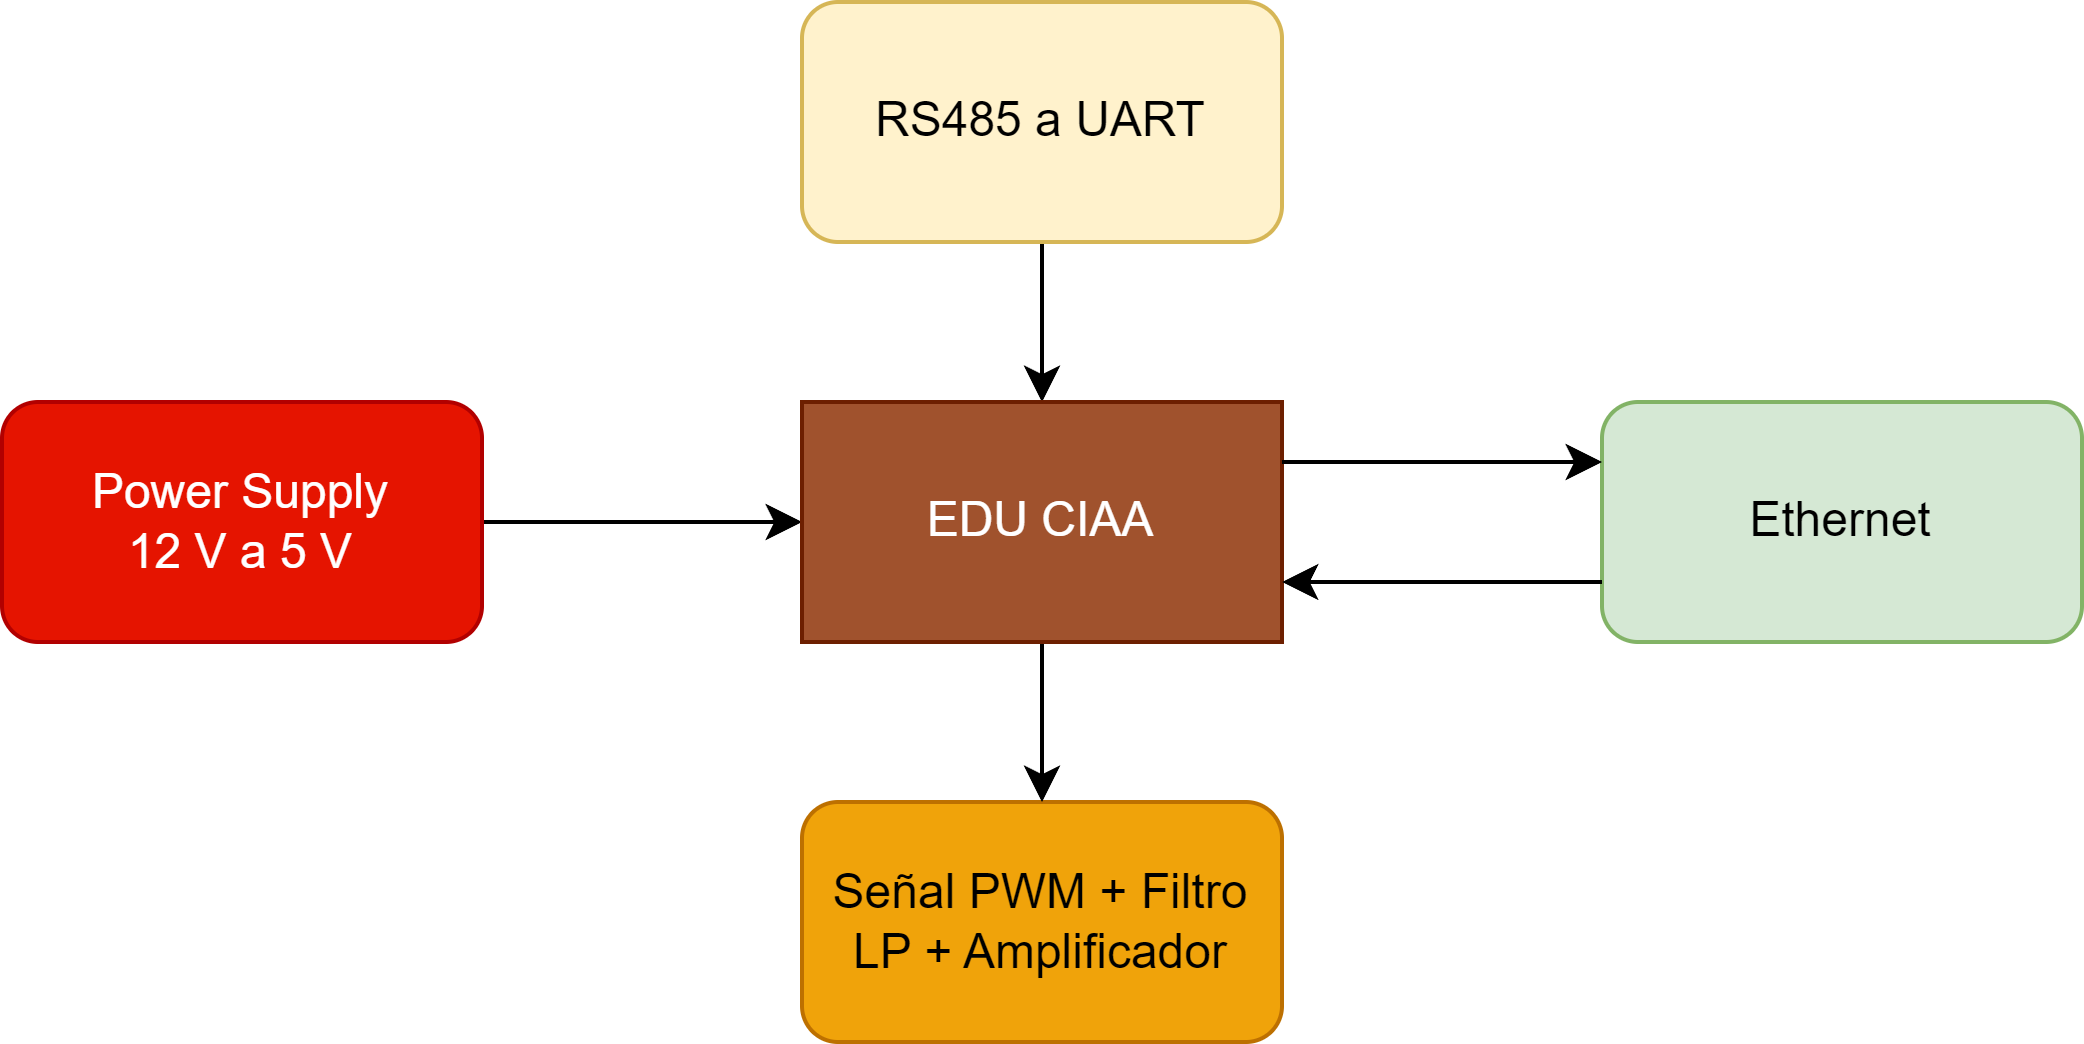
\includegraphics[width=0.85\linewidth]{Figuras/datalogger/esquemaHardarware.png}
    \caption{Diagrama en bloques del sistema electrónico.}
    \label{fig:esquemaHardarware}
\end{figure}




\section{Desarrollo del Hardware}\label{sec:desarrolloHardware}


Para el desarrollo del Hardware, en una primera etapa se realizó un proceso de investigación de hojas de datos, manuales, artículos y videos de internet para ver qué módulos y componentes comprar para la implementación de la aplicación. Además, se utilizaron herramientas como LT Spice para la simulación de circuitos y KiCad para el diseño de PCB. 

La placa de desarrollo EDU-CIAA-NXP, se muestra en la Figura \ref{fig:EduCiaaPlaca}, es una versión de bajo costo de la CIAA-NXP \cite{proyectoCIAA} pensada para la enseñanza universitaria, terciaria y secundaria. 
\begin{figure}[H]
    \centering
    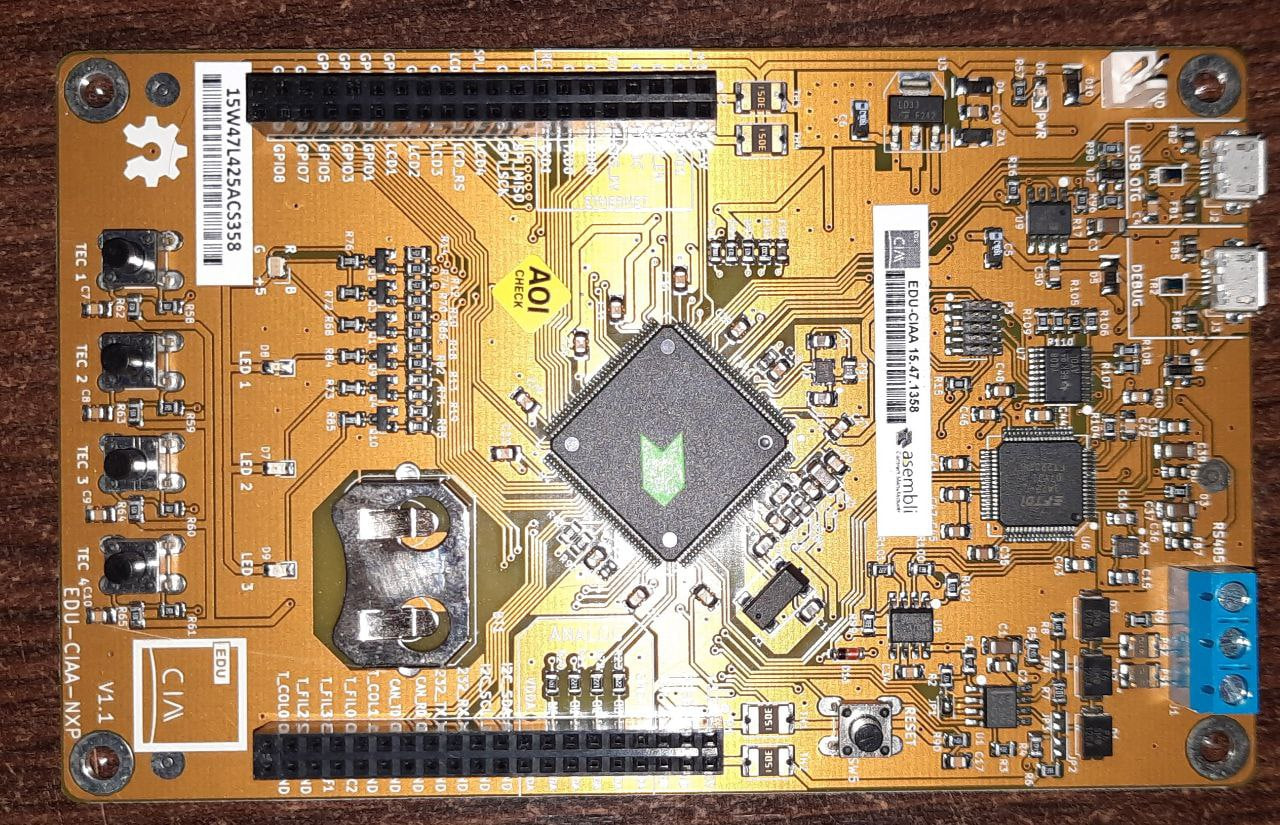
\includegraphics[width=0.8\linewidth]{Figuras/datalogger/Hardware/EduCiaaPlaca.jpg}
    \caption{Placa de desarrollo EDU CIAA}
    \label{fig:EduCiaaPlaca}
\end{figure}
El desarrollo se centró en esta placa, que cuenta con las siguientes especificaciones 


\begin{itemize}[leftmargin=*]

  \item \textbf{Microcontrolador LPC4337:}
    \begin{itemize}[label=-]
      \item \textbf{Núcleos:} Dual-core ARM Cortex-M4/M0.
      \item \textbf{Velocidad de reloj:} Hasta 204 MHz.
      \item \textbf{Memoria RAM:} Hasta 264 KB.
      \item \textbf{Memoria Flash:} Hasta 1 MB.
    \end{itemize}

  \item \textbf{Puertos micro-USB:}
    \begin{itemize}[label=-]
      \item Uno para aplicaciones y debugging (DEBUG).
      \item Otro para alimentación (OTG).
    \end{itemize}
  
  \item \textbf{Salidas digitales:}
    \begin{itemize}[label=-]
      \item 4 salidas digitales implementadas con LEDs RGB.
    \end{itemize}
  
  \item \textbf{Entradas digitales:}
    \begin{itemize}[label=-]
      \item 4 entradas digitales con pulsadores.
    \end{itemize}
  
  \item \textbf{Comunicaciones RS485:}
    \begin{itemize}[label=-]
      \item Puerto de comunicaciones RS-485 con bornera.
    \end{itemize}
  
  \item \textbf{Conector de expansión P1:}
    \begin{itemize}[label=-]
      \item 3 entradas analógicas con 10 Bits de resolución cada uno (ADC0, 1, 2 y 3).
      \item 1 salida analógica (DAC0).
      \item 1 puerto I2C.
      \item 1 puerto asincrónico full duplex (para RS-232).
      \item 1 puerto CAN.
      \item 1 conexión para un teclado de 3×4.
    \end{itemize}
  
  \item \textbf{Conector de expansión P2:}
    \begin{itemize}[label=-]
      \item 1 puerto Ethernet.
      \item 1 puerto SPI.
      \item 1 puerto para display LCD con 4 bits de datos, Enable y RS.
      \item 9 pines genéricos de I/O.
    \end{itemize}
    
\end{itemize}
En la Figura \ref{fig:EDU_CIAA_esquema} se describe un diagrama en bloques de la placa
\begin{figure}[H]
    \centering
    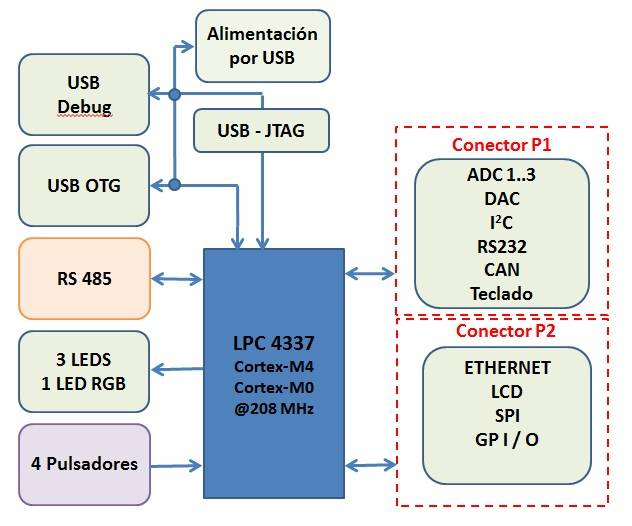
\includegraphics[width=0.7\linewidth]{Figuras/datalogger/Hardware/EDUCIAAesquema.png}
    \caption{Diagrama en bloques de la EDU-CIAA}
    \label{fig:EDU_CIAA_esquema}
\end{figure}

El SMN proporcionó los sensores de viento de ultrasonido. Se trabajó con los siguientes anemómetros: el modelo WMT700 de la marca VAISALA, Figura \ref{fig:sensorVaisala}
, utilizado como anemómetro patrón, y el modelo HD51.3D de la marca Delta OHM, Figura \ref{fig:sensorDeltaOhm}, utilizado como anemómetro bajo calibración. Ambos sensores operan con la interfaz eléctrica RS485 y vienen con un cable de aproximadamente 15 metros, puesto que estos sensores se instalan en torres de 10 metros de altura.

\begin{figure}[H]
    \centering
    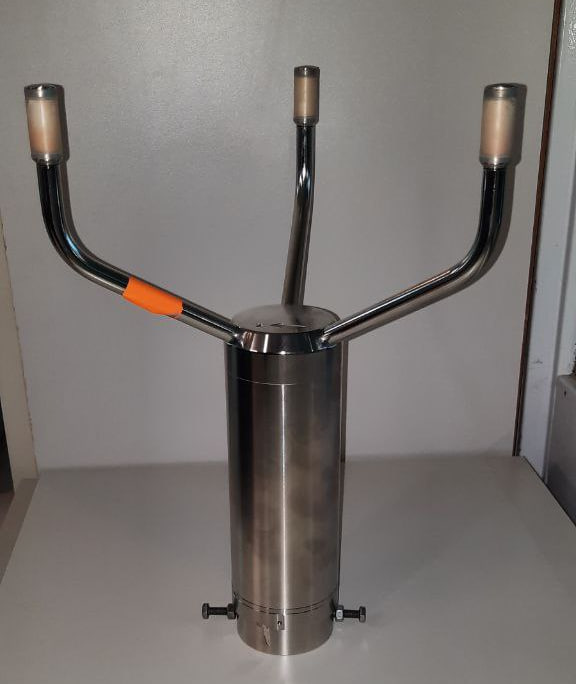
\includegraphics[width=0.4\linewidth]{Figuras/datalogger/Hardware/sensorVaisala.jpg}
    \caption{Sensor Vaisala modelo WMT700}
    \label{fig:sensorVaisala}
\end{figure}


\begin{figure}[H]
    \centering
    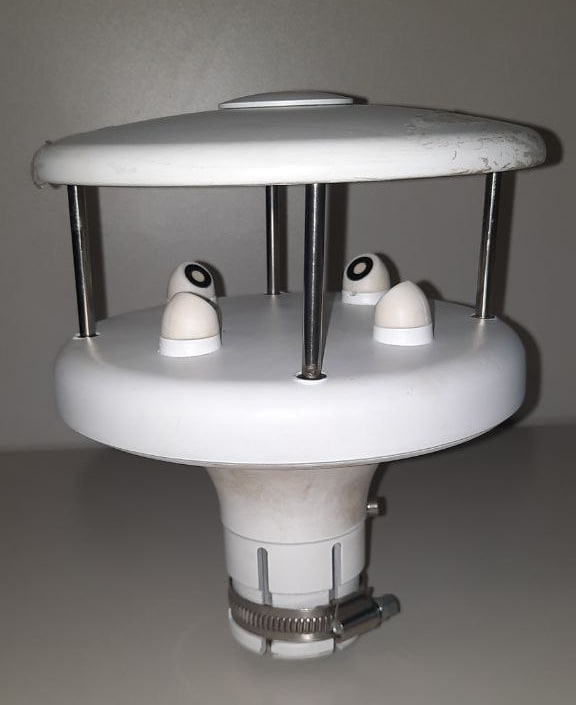
\includegraphics[width=0.4\linewidth]{Figuras/datalogger/Hardware/sensorDeltaOhm.jpg}
    \caption{Sensor Delta OHM modelo HD51.3D}
    \label{fig:sensorDeltaOhm}
\end{figure}
 Algunas especificaciones técnicas de este tipo de anemómetros se muestran en la tabla \~ref{tab:especTecniDelta}. Las más relevantes para el proceso de calibración son, el rango de medición, la resolución, la precisión, los protocolos de comunicación, la alimentación eléctrica y el intervalo de tiempo mínimo con el que puede tomar muestras. 

%%%%%%%%%%%%%%%%%%%%%%%%%%%%%%%%%%%%%%%%%%%%%%%%%%%%%%%%%%%%%%%%%%%%%%%%%%%%%%%%%%%%%%%%%%%%%%%%%%%%%%%
\subsection{Módulo de alimentación electrica}\label{sec:moduloAlimentacionElectrica}

Los anemómetros funcionan con una alimentación de 12 \unit{\volt} para el sistema principal y 24 \unit{\volt} para el sistema de calefacción ya que estos sensores pueden ser expuestos a entornos con temperaturas por debajo de cero grados. Por otro lado, los módulos Ethernet, RS-485 y los amplificadores operacionales trabajan con 5 \unit{\volt}, mientras que el resto de la placa de desarrollo opera con 3.3 \unit{\volt}. Por esta razón, se decide alimentar todo el sistema con una fuente de 12 \unit{\volt}, para garantizar el funcionamiento de los anemómetros en condiciones normales de temperatura dentro del laboratorio.rwer

Para lograr estos niveles de tensión, se optó por un regulador basado en el chip LM2596S (Step-Down), como se indica en la Figura \ref{fig:StepDowmLM2596S}
. Se conectan 12 \unit{\volt} a la entrada y se ajusta el potenciómetro hasta obtener 5 \unit{\volt} a la salida. Esta salida estará disponible para conectar el resto de los módulos.

Cabe aclarar que, si bien la CIAA tiene una salida de 5 \unit{\volt}, esta no proporciona la corriente suficiente para alimentar todos los módulos, ya que está limitada por los 500 \unit{\milli\ampere} que entrega un puerto USB 2.0. En contraste, el regulador DC-DC basado en el LM2596 puede entregar hasta 3 \unit{\ampere}, satisfaciendo así las necesidades de corriente de todos los módulos conectados. 
% Todo el sistema tiene un consumo de -- \unit{\milli\ampere}

\begin{figure}[H]
    \centering
    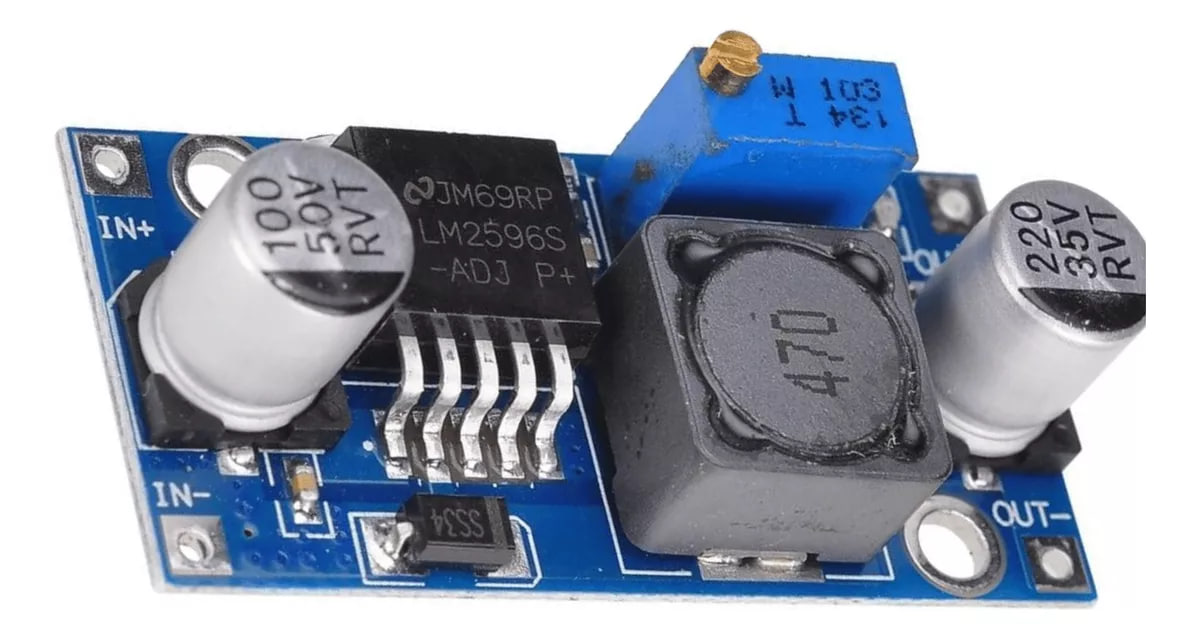
\includegraphics[width=0.6\linewidth]{Figuras/datalogger/Hardware/StepDowmLM2596S.jpg}
    \caption{Regulador de voltaje DC-DC basado en el chip LM2596.}
    \label{fig:StepDowmLM2596S}
\end{figure}

En la Figura \ref{fig:esquemPowerSupply} se observa el esquemático del sistema, mostrando cómo se conecta el módulo LM2596 con el resto de los componentes. Este esquemático incluye un divisor resistivo y un diodo Zener de 3.3 \unit{\volt} para limitar y adaptar la tensión de 12 \unit{\volt} a un rango de 3.3 \unit{\volt}, ya que se toman muestras de la tensión de alimentación a través del canal analógico-digital ADC\_CH1 de la EDU-CIAA. Esta información de la tensión se envía junto con los datos de los anemómetros, permitiendo un monitoreo preciso del sistema de alimentación. Además, se han agregado filtros de bypass a la alimentación del amplificador operacional LM358 para asegurar una operación estable y sin ruido.

\begin{figure}[H]
    \centering
    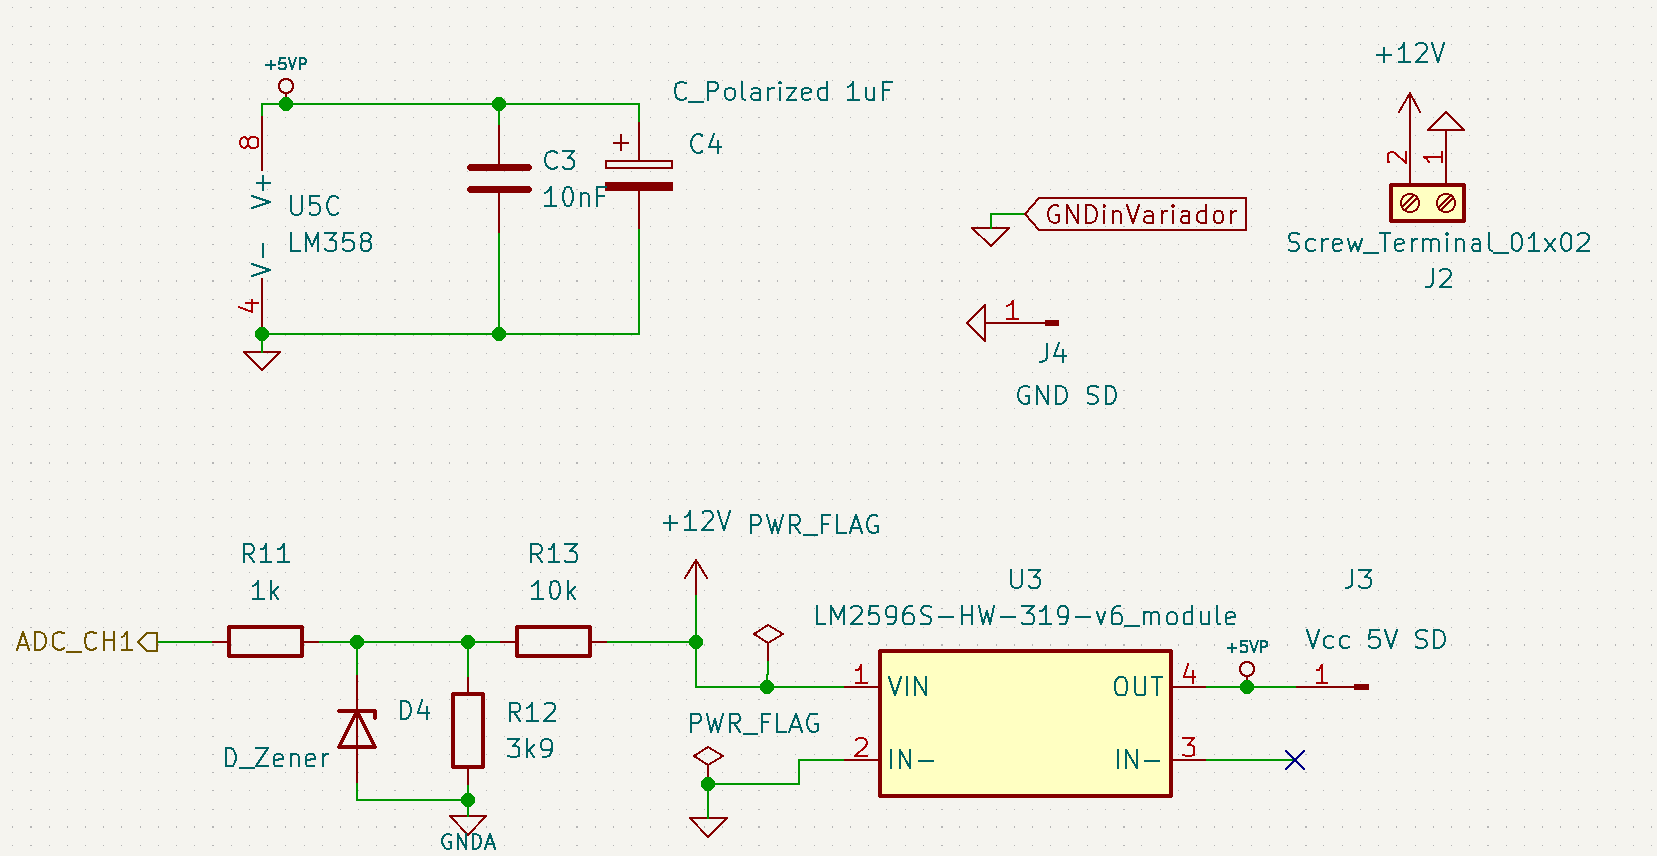
\includegraphics[width=0.9\linewidth]{Figuras/datalogger/Hardware/esquemPowerSupply.png}
    \caption{Esquemático del sistema de alimentación con módulo LM2596, diodo Zener, divisor resistivo y filtros de bypass para el LM358.}
    \label{fig:esquemPowerSupply}
\end{figure}

%%%%%%%%%%%%%%%%%%%%%%%%%%%%%%%%%%%%%%%%%%%%%%%%%%%%%%%%%%%%%%%%%%%%%%%%%%%%%%%%%%%%%%%%%%%%%%%%%%%%%%%
\subsection{Módulo de adquisición de datos de viento}\label{sec:moduloAdquisicionDatoViento}

En la sección \ref{sec:instrumentos_med_viento} del capítulo \ref{cap:viento} describimos los distintos tipos de sensores para medir la intensidad y dirección del viento. En particular se trabajó con anemómetros de ultrasonido cuya interfaz electrónica utiliza el protocolo RS-485, el mismo es un protocolo diferencial ampliamente utilizado en entornos industriales debido a su robustez y confiabilidad. Utiliza tres cables (A, B y GND) y transmite datos mediante la diferencia de voltaje entre A y B, ofreciendo alta inmunidad al ruido. Algunas características del protocolo son:

\begin{itemize}
    \item Tensión diferencial entre A y B para la transmisión de datos. Cuando la línea A es más positiva que la línea B por al menos 200 mV, se interpreta como un estado lógico '1'. Inversamente, cuando la línea B es más positiva que la línea A por al menos 200 mV, se interpreta como un estado lógico '0'.
    \item Velocidades de hasta 10 Mbps y distancia de hasta 1200 metros.
    \item Soporte para multidrop de hasta 32 dispositivos.
    \item Resistencias de terminación de 120 ohmios para minimizar reflexiones de señal.
    \item Robustez contra interferencias eléctricas en entornos industriales.
\end{itemize}

En la Figura \ref{fig:rs485DeltaOhm} se muestra un esquema de conexión para el sensor DELTA OHM HD51.3D el cual fue utilizado para conectar dicho sensor al sistema. En particular, nos interesa dos cables para la alimentacion V+ (12 \unit{\volt}) y V- (GND), y tres cables para los datos, DATA+ (A), DATA- (B) y GND

\begin{figure}[H]
    \centering
    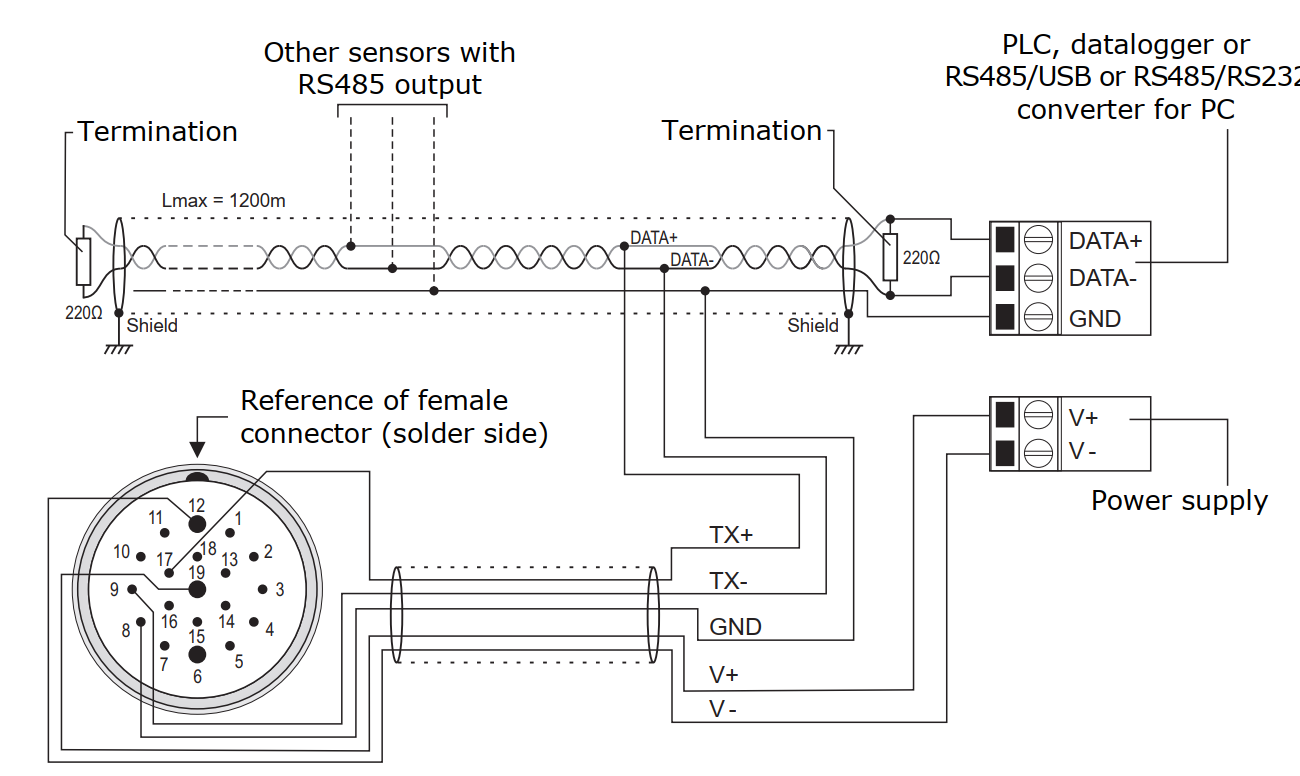
\includegraphics[width=0.9\linewidth]{Figuras/datalogger/Hardware/rs485DeltaOhm.png}
    \caption{Esquema de conexión de datos y alimentación del sensor HD51.3D con un Datalogger o un PLC.}
    \label{fig:rs485DeltaOhm}
\end{figure}
La placa EDU-CIAA cuenta con un módulo RS-485 integrado, como se muestra en la Figura \ref{fig:rs485CIAA}. El anemómetro patrón WMT700 se conectó directamente a esta bornera. El sensor envía datos en modo ráfaga cada segundo, lo que permite una comunicación directa y eficiente sin necesidad de adaptadores adicionales.
\begin{figure}[H]
    \centering
    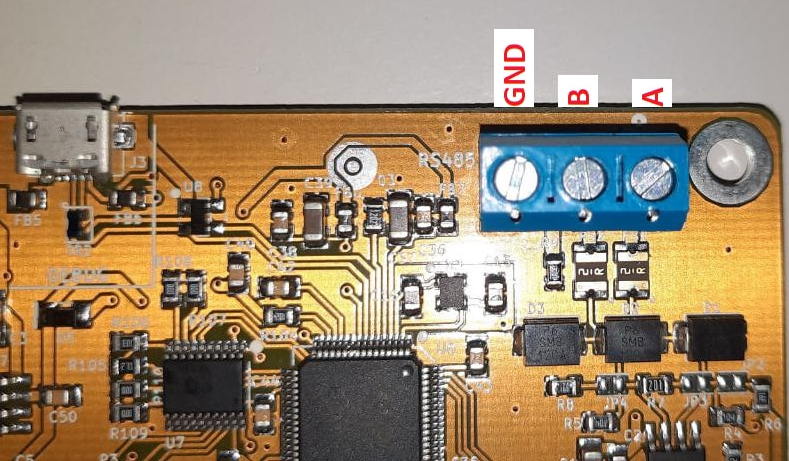
\includegraphics[width=0.4\linewidth]{Figuras/datalogger/Hardware/rs485CIAA.jpg}
    \caption{Puerto RS-485 integrado en la EDU-CIAA}
    \label{fig:rs485CIAA}
\end{figure}

Para conectar el anemómetro bajo calibración se utilizó el módulo MAX485, Figura \ref{fig:moduleMax485}, que convierte las señales RS-485 a niveles de la UART (TTL). 

\begin{figure}[H]
    \centering
    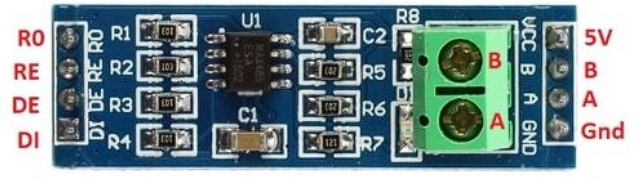
\includegraphics[width=0.55\linewidth]{Figuras/datalogger/Hardware/moduleMax485.png}
    \caption{Módulo convertidor de RS485 a UART (TTL)}
    \label{fig:moduleMax485}
\end{figure}
Los pines del módulo tienen la siguiente descripción:

\begin{itemize}
    \item \textbf{Pin A y B:} Conectan los cables A y B del sensor RS-485.
    \item \textbf{Pin GND:} Conexión a tierra para la alimentación y la señal.
    \item \textbf{Pin RO (Receiver Output):} Salida de datos recibidos. Entrega los datos TTL recibidos del sensor RS-485 convertidos por el MAX485.
    \item \textbf{Pin DI (Driver Input):} Entrada de datos de transmisión TTL hacia el módulo MAX485 para ser convertidos a señales RS-485.
    \item \textbf{Pin DE (Driver Enable):} Controla la transmisión de datos. Se activa para habilitar la transmisión de datos desde el pin DI.
    \item \textbf{Pin RE (Receiver Enable):} Controla la recepción de datos. Se activa para habilitar la recepción de datos en el pin RO.
\end{itemize}

Como se muestra en la Figura \ref{fig:esquemRS485}, el módulo MAX485 se alimentó con 5 \unit{\volt} suministrados por el regulador LM2596S. Desde un extremo, se conectaron los cables A y B del sensor RS-485, mientras que del otro lado se conectó a la UART-RS232 de la EDU-CIAA. Para adaptar la señal TTL a la placa de desarrollo, se utilizó un resistor de 1 \unit{\kilo\ohm} entre el pin RO del MAX485 y la UART-RS232.

Los pines DE y RE del MAX485 se conectaron a GND para permitir la recepción de datos desde el sensor hacia la placa, operando en modo ráfaga, enviando datos cada un segundo. El pin DI no se conectó, ya que el sensor no requiere recibir datos o comandos desde la EDU-CIAA.

\begin{figure}[H]
    \centering
    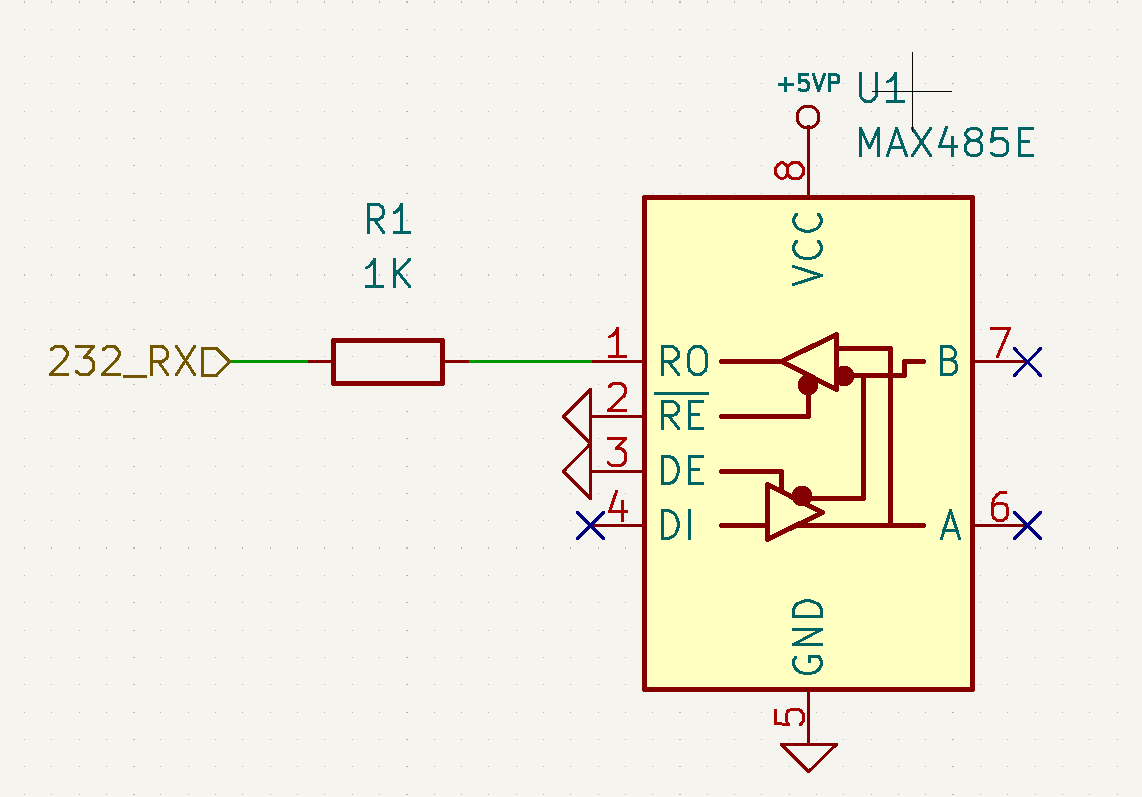
\includegraphics[width=0.7\linewidth]{Figuras/datalogger/Hardware/esquemRS485.png}
    \caption{Esquemático del módulo MAX485 para la recepción de datos del sensor bajo calibración.}
    \label{fig:esquemRS485}
\end{figure}


%%%%%%%%%%%%%%%%%%%%%%%%%%%%%%%%%%%%%%%%%%%%%%%%%%%%%%%%%%%%%%%%%%%%%%%%%%%%%%%%%%%%%%%%%%%%%%%%%%%%%%%
% Explicar el protocolo y tensiones de los anemometros
% Poner un esquema de módulo y como va conectado a la CIAA
%%%%%%%%%%%%%%%%%%%%%%%%%%%%%%%%%%%%%%%%%%%%%%%%%%%%%%%%%%%%%%%%%%%%%%%%%%%%%%%%%%%%%%%%%%%%%%%%%%%%%%%
\subsection{Módulo de comunicación Ethernet/SPI  }\label{sec:moduloEthernet}

Para comunicar el sistema embebido con distintos servidores, como el servidor WebSocket desarrollado en la sección \ref{sec:back_end}, así como servidores NTP para sincronizar la fecha y hora, se utilizó el módulo W5100, Figura \ref{fig:moduleW5100}. Este módulo emplea el protocolo TCP/IP para proporcionar una comunicación estable. Se alimenta con 5 \unit{\volt} y utiliza una interfaz SPI para comunicarse con la placa de desarrollo.

Una de las principales ventajas del módulo W5100 \cite{W5100Datasheet} es su capacidad para manejar cuatro sockets independientes, lo que permite conectarse a hasta cuatro servidores distintos de manera concurrente. Esto mejora la eficiencia y la flexibilidad del sistema, facilitando la integración con múltiples servicios de red simultáneamente.



\begin{figure}[H]
    \centering
    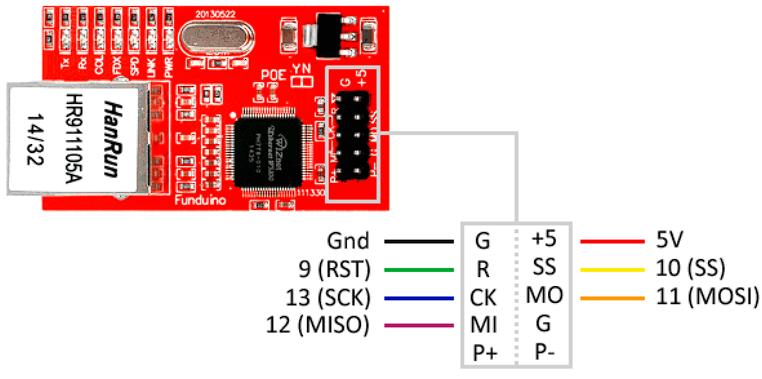
\includegraphics[width=0.7\linewidth]{Figuras/datalogger/Hardware/moduleW5100.png}
    \caption{Módulo W5100 utilizado para realizar la conectividad a internet a través de la interfaz SPI del microcontrolador.}
    \label{fig:moduleW5100}
\end{figure}
Descripción de los Pines del Módulo W5100 Ethernet
\begin{itemize}
\item \textbf{VCC:} Pin de alimentación, generalmente conectado a 3.3V o 5V, dependiendo del módulo específico.
\item \textbf{GND:} Pin de tierra, utilizado para completar el circuito de alimentación.
\item \textbf{MISO (Master In Slave Out):} Pin de salida de datos del módulo hacia el microcontrolador en la comunicación SPI.
\item \textbf{MOSI (Master Out Slave In):} Pin de entrada de datos desde el microcontrolador hacia el módulo en la comunicación SPI.
\item \textbf{SCK (Serial Clock):} Pin de reloj serial utilizado para sincronizar la comunicación SPI.
\item \textbf{SS (Slave Select):} Pin utilizado por el microcontrolador para seleccionar el módulo W5100 como dispositivo esclavo en la comunicación SPI.
\item \textbf{RST (Reset):} Pin de reinicio, utilizado para reiniciar el módulo.
\item \textbf{P+ y P-:} Pines para Power over Ethernet (PoE), utilizados para suministrar energía al dispositivo a través del cable Ethernet.
\end{itemize}

Como se muestra en la Figura \ref{fig:esquemEthernet}, el módulo W5100 se alimentó con 5 \unit{\volt} y se conectaron los pines del módulo W5100 a la EDU-CIAA de la siguiente manera: el pin MO a SPI\_MOSI, el pin MI a SPI\_MISO, y el pin SCK a SPI\_SCK. Además, se conectó el pin NSS al GPIO1 para poder reiniciar el módulo cuando sea necesario por software. El resto de los pines del módulo quedaron sin conectar.

Con esta configuración, se logró una comunicación bidireccional, permitiendo transmitir datos de los sensores de viento desde el datalogger hacia la aplicación web, así como recibir comandos desde la aplicación web hacia el datalogger.
\begin{figure}[H]
    \centering
    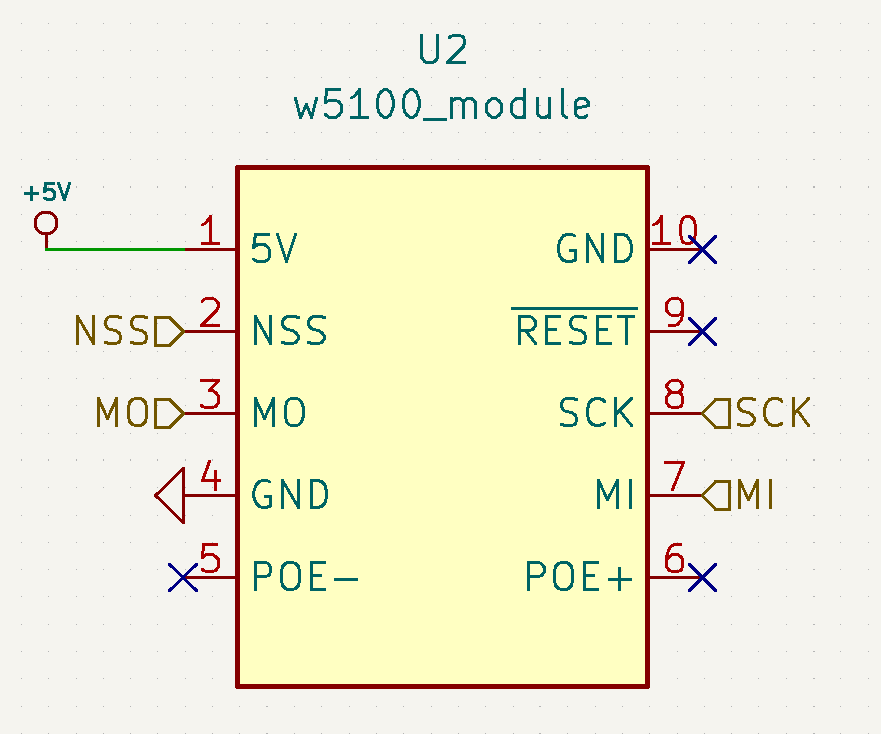
\includegraphics[width=0.7\linewidth]{Figuras/datalogger/Hardware/esquemEthernet.png}
    \caption{Esquemático del módulo W5100 para la comunicación bidireccional con distintos servidores.}
    \label{fig:esquemEthernet}
\end{figure}


%%%%%%%%%%%%%%%%%%%%%%%%%%%%%%%%%%%%%%%%%%%%%%%%%%%%%%%%%%%%%%%%%%%%%%%%%%%%%%%%%%%%%%%%%%%%%%%%%%%%%%%
\subsection{Circuito PWM}\label{sec:circuitoPWM}


En esta sección, se presenta el desarrollo de un circuito que permite controlar la potencia del motor del túnel de viento a través de modulación por ancho de pulso (PWM, por sus siglas en inglés). Primero, se describe el funcionamiento original del variador de velocidad. En la Figura \~ref{fig:esquemCircuitoControlTunel} se muestra un esquema del tablero de control del variador de velocidad del túnel de viento.

El tablero posee dos pulsadores: uno de marcha (BT1-NC) y otro de parada (BT2-NA), que permiten encender y apagar, respectivamente, el conjunto variador-motor del túnel de viento. Además, cuenta con dos voltímetros de corriente continua, V1 y V2, que muestran el valor de tensión que se está aplicando al motor.

La velocidad del viento se regula manualmente mediante dos potenciómetros lineales: $P1 = \SI{1}{\kilo\ohm}$ y $P2 = \SI{500}{\ohm}$. Además, el circuito incluye una resistencia $R1 = \SI{1.2}{\kilo\ohm}$ conectada a la fuente $VCC = \SI{10}{\volt}$ del variador. Estos componentes, junto con los potenciómetros, forman un divisor de tensión variable que permite ajustar la tensión entre \SI{0}{\volt} y \SI{10}{\volt}, la cual se aplica al pin $VADC$.

Se realizó una medición con un amperímetro en serie con la resistencia $R1$ y se obtuvo que la corriente que pasa por $R1$ cuando se ajusta el potenciómetro para obtener una $VADC = \SI{3.56}{\volt}$ es de \SI{140}{\micro\ampere}. Cuando se ajusta el potenciómetro para obtener una $VADC = \SI{5}{\volt}$, la corriente es de \SI{200}{\micro\ampere}. Con estas mediciones podemos concluir que el pin $VADC$ del variador tiene una resistencia de entrada de alta impedancia, ya que el consumo de corriente no supera los \SI{500}{\micro\ampere}.



%     Aca explicar como funcion el tunnel actualmente con los ponteciometros y como con el diseño de este circuito PWM logramos reemplazar los potes
% Rango de tensiones del Vadc para alcanzar la maxima velocidad y rango real VCC = 10

% quiza poner tabla para ver que esta fuente esta limitada por corriente y dcir porque no usamos esta, poner tabla de tension vs corriente.



\begin{figure}[H]
    \centering
    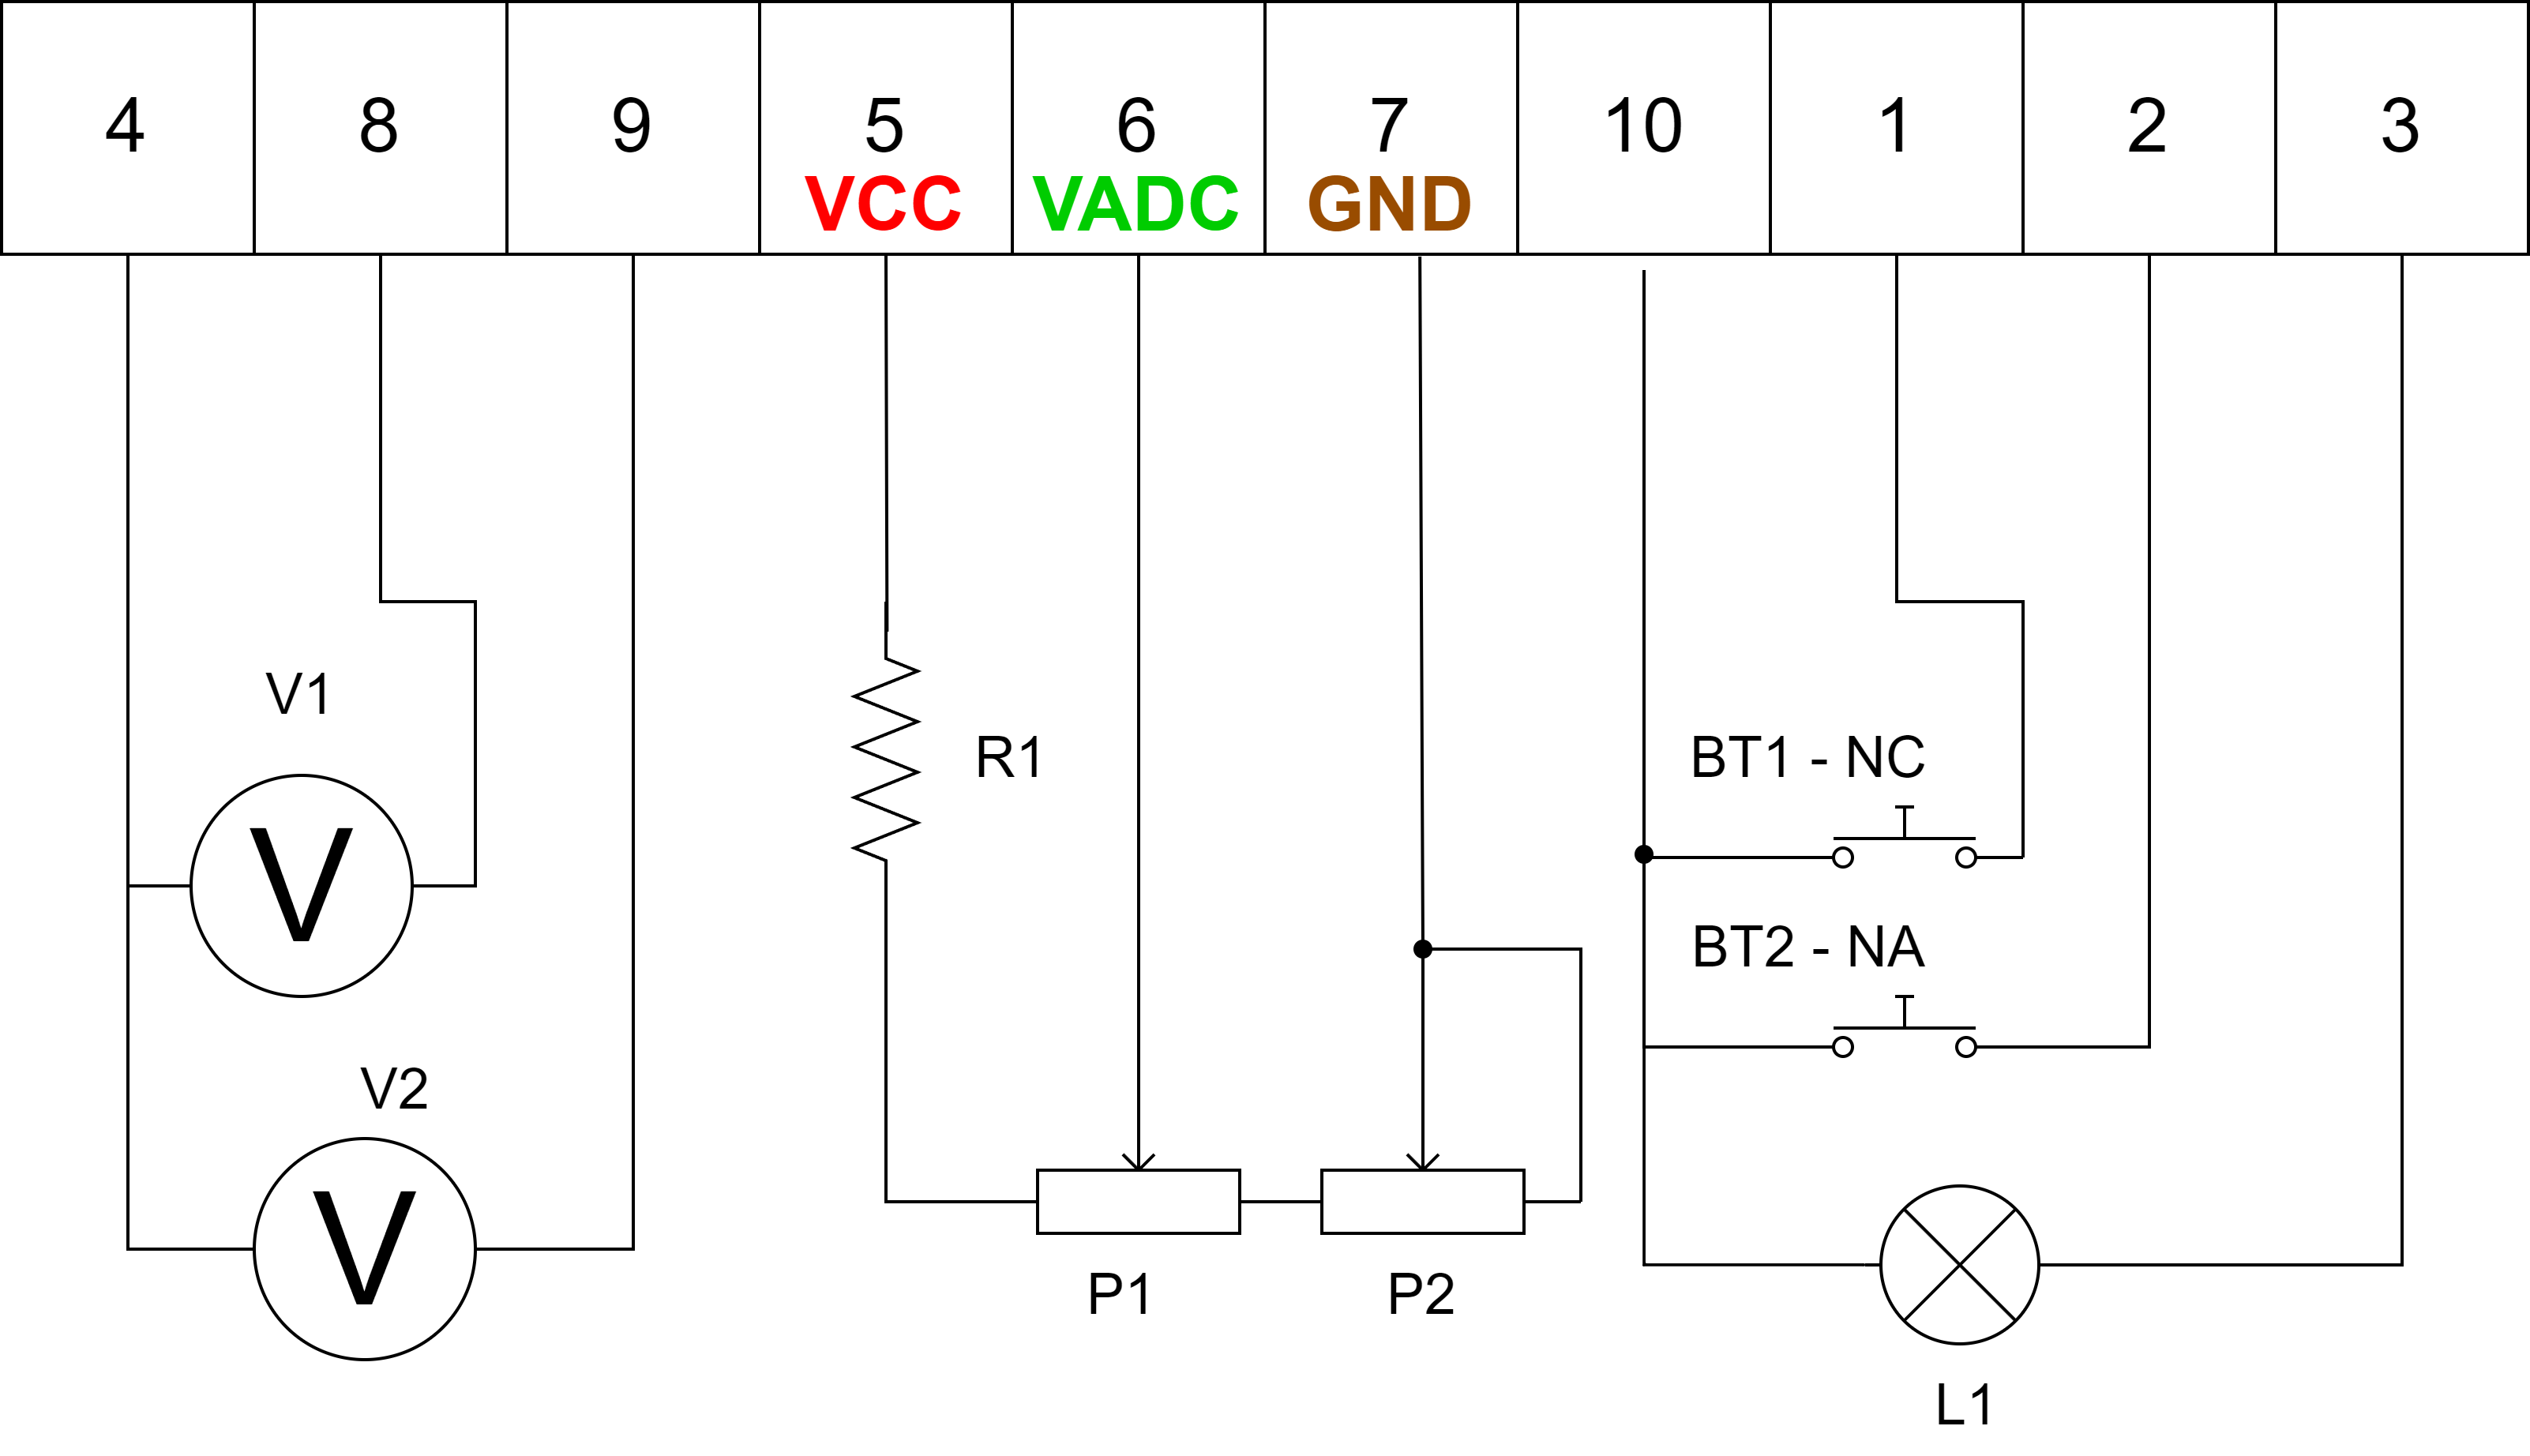
\includegraphics[width=0.7\linewidth]{Figuras/datalogger/Hardware/esquemCircuitoControlTunel.png}
    \caption{Esquemático circuital del tablero de control del tunel de viento.}
    \label{fig:esquemCircuitoControlTunel}
\end{figure}

Para lograr controlar el nivel de tensión $VADC$ por medio de software, se remplazó los dos potenciómetros y el resistor $R1$ por un circuito diseñado en la siguiente sección. Por otro lado, se hizo un relevamiento de la corriente máxima que puede entregar la fuente del variador $VCC$ conectando distintos valores de resistencia entre $VCC$ y $GND$. Los resultados se muestran en la tabla \ref{tab:currentVccVariador}. Como se aprecia a medida que disminuimos la carga $R$, tanto la tensión, como la corriente que puede entregar la fuente, disminuye y la corriente máxima que puede entregar esta fuente es de $\SI{100}{\milli\ampere}$, con una tensión de $\SI{2.29}{\volt}$. Tomando como referencia el consumo de corriente y la tensión que precisa el datalogger, esta fuente $VCC$ del variador no es capaz de suministrar la corriente necesaria y mantener la tensión constante, por esta razón se optó por alimentar el sistema como se explicó en la sección \ref{sec:moduloAlimentacionElectrica}



\begin{table}[H]
\centering
\begin{tblr}{
  cells = {c},
  row{1} = {Sail},
  hlines,
  vlines,
}
\textbf{R [\unit{\ohm}]} & \textbf{VCC [\unit{\milli\volt}]} & \textbf{I\_R[\unit{\milli\ampere}]} \\
47K              & 9.9               & 2               \\
10K              & 9.52              & 5.9               \\
1K               & 9.29              & 9.4               \\
560              & 7.55              & 13.48             \\
330              & 5.63              & 16.97             \\
100              & 2.29              & 100               \\
47               & 859               & 100               
\end{tblr}
\caption{Mediciones de tensión y corriente de la fuente del variador para distintas resistencias de carga.}
\label{tab:currentVccVariador}
\end{table}

\subsubsection{Simulación del circuito}\label{simulacionCircuito}

En la Figura \ref{fig:pwmCircuitSimulate} se muestra el diseño del circuito del PWM \cite{EEVblog225}, que reemplaza al divisor de tensión formado por los potenciómetros $P1$, $P2$ y la resistencia $R1$, mostrado en la Figura \ref{fig:esquemCircuitoControlTunel}. La señal de entrada es una señal PWM (cuadrada) obtenida desde un pin de la EDU-CIAA. Esta señal, para un ciclo de trabajo del $100\%$, tiene una amplitud de $\SI{3.3}{\volt}$ acorde con los niveles digitales de tensión de la EDU-CIAA. 

Luego, esta señal pasa por dos etapas de filtrado, cada una con una frecuencia de corte de $\SI{1592}{\hertz}$. Con esta doble etapa de filtro pasa bajo, se obtiene una señal continua con menor rizado, como se muestra en la Figura \ref{fig:filter1and2} (señal verde y azul).

Posteriormente, la señal rectificada ingresa a una etapa de amplificación no inversora, implementada con el amplificador operacional LM358. Este nivel de continua es el que se conecta al pin $VADC$ del variador de velocidad del túnel de viento. La señal a la salida del amplificador tiene una ganancia de $\frac{\SI{3.5}{\volt}}{\SI{3.3}{\volt}} \approx \SI{1.06}{}$. Se decidió amplificar hasta $\SI{3.5}{\volt}$ porque se encontró que la máxima velocidad que logra alcanzar el túnel, de $\SI{25}{\meter\per\second}$, se alcanza con $\SI{3.5}{\volt}$ a la entrada del $VADC$. Esta limitación viene dada por la mecánica del motor, por lo tanto, en estas condiciones no es necesario amplificar a valores mayores de $\SI{3.5}{\volt}$, ya que el túnel no incrementa su velocidad de viento.

No obstante, para cuando se mejore la mecánica y transmisión del motor del túnel de viento, se dejó un resistor variable (Preset) $R3=\SI{10}{\kilo\ohm}$. Con este preset se cambia la ganancia del amplificador. Se lo ajustó para alcanzar $\SI{3.5}{\volt}$ a la salida del operacional, y podrá ser recalibrado para alcanzar mayores niveles de tensión, lo que genera, mayores velocidades de viento.

\begin{figure}[H]
    \centering
    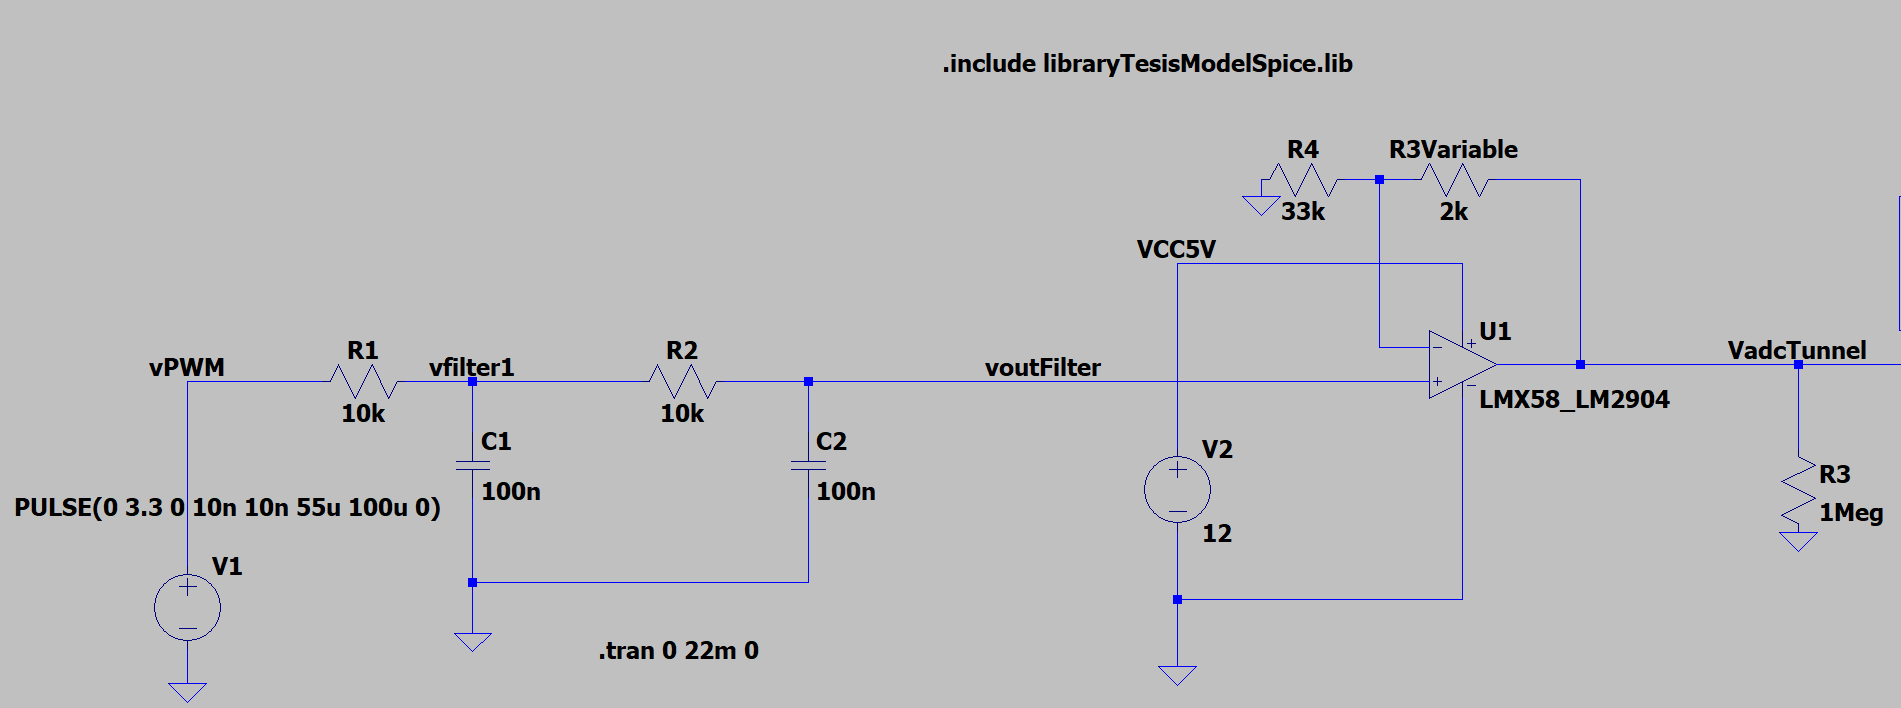
\includegraphics[width=1\linewidth]{Figuras/datalogger/Hardware/pwmCircuitSimulate.png}
    \caption{Circuito diseñado para obtener distintos niveles de tensión mediante la variación del ciclo de trabajo de una señal cuadrada (PWM).}
    \label{fig:pwmCircuitSimulate}
\end{figure}


\begin{figure}[H]
    \centering
    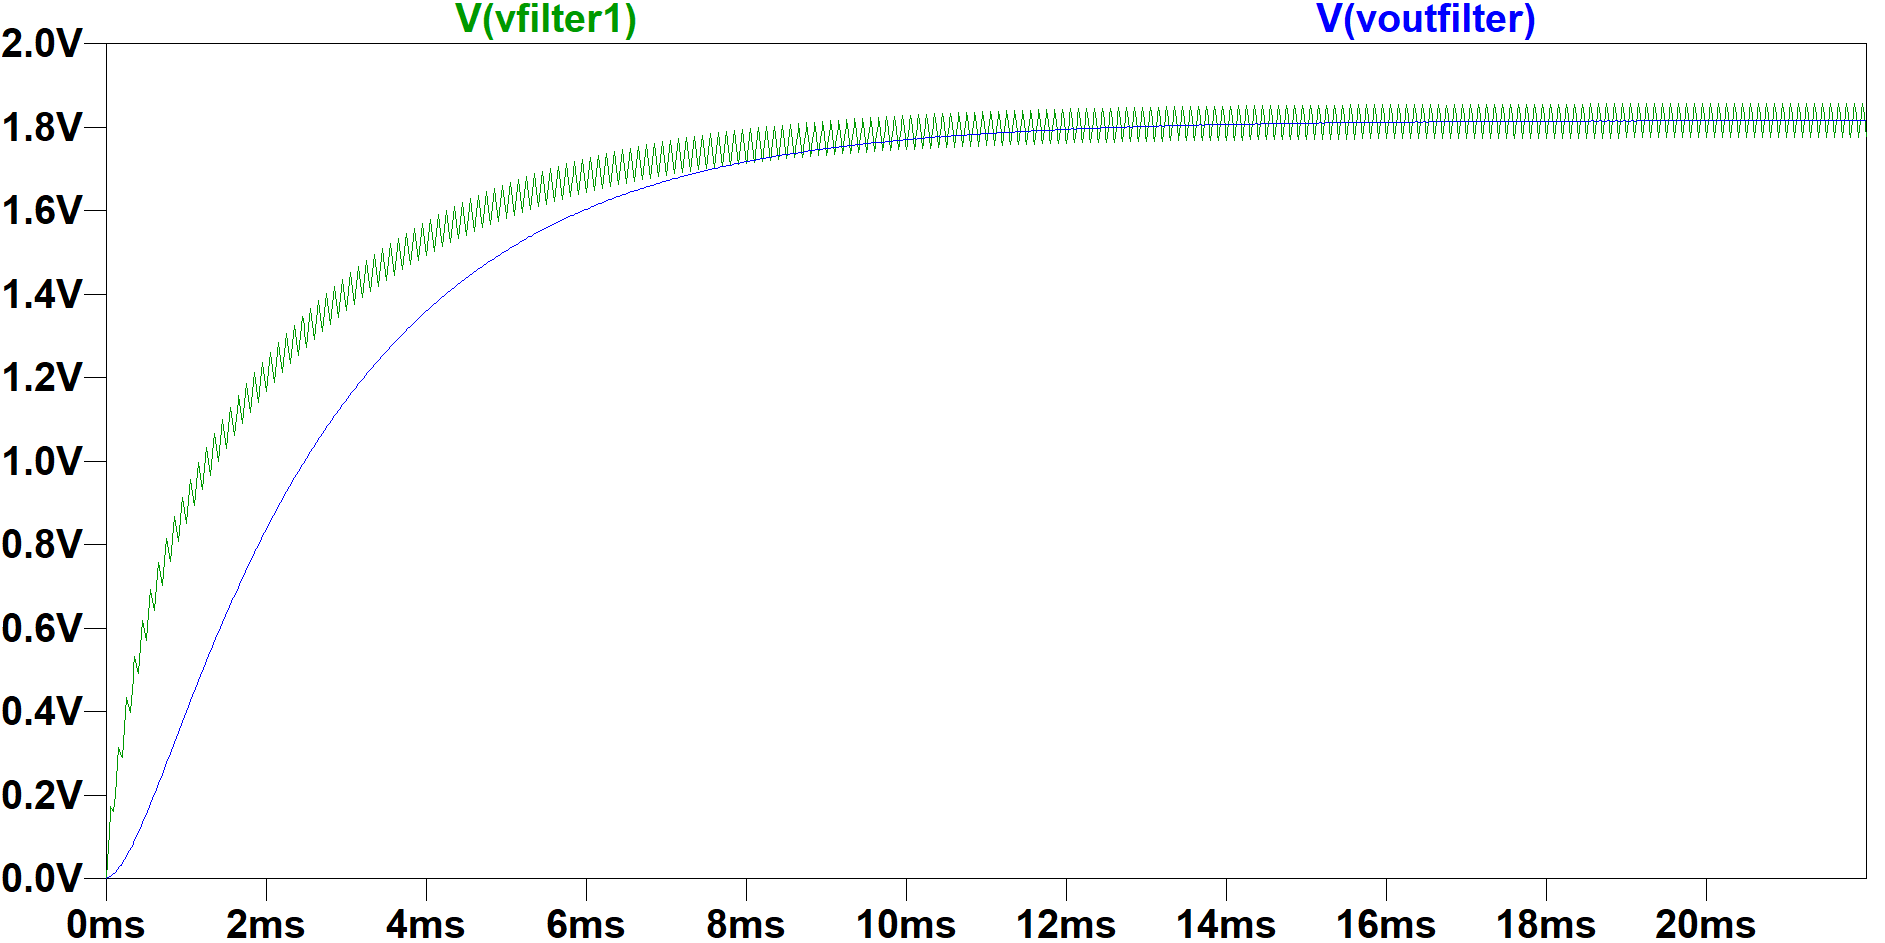
\includegraphics[width=1\linewidth]{Figuras/datalogger/Hardware/filter1and2.png}
    \caption{Circuito diseñado para obtener distintos niveles de tensión mediante la variación del ciclo de trabajo de una señal cuadrada (PWM).}
    \label{fig:filter1and2}
\end{figure}

% En la figura \ref{fig:adc100PercentPwm} se muestra el resultado de la simulación para un pulso $vPWM$ (señal azul) de $ \SI{100}{\micro\second}$ de periodo y una amplitud de $\SI{3.3}{\volt}$ con el ciclo de trabajo al $99\%$.La tensión $vFilter1$ (señal verde) en la primera etapa del filtro pasa bajo, tiene un tiempo de crecimiento corto del orden de los $\SI{10}{\milli \second}$, pero mayor ripple. La segunda etapa del filtro es la tensión $voutFilter$ (señal roja), esta señal tiene un mayor tiempo de crecimiento del orden $\SI{16}{\milli \second}$, pero un rizado mucho menor, entonces el agregado de otra etapa de filtrado permite obtener un nivel de continua con rizado mucho menor. Finalmente, podemos observar la señal $vadcTunel$ (señal celeste), esta señal es estable y se la conecta al $VADC$ del variador de velocidad.


En la Figura \ref{fig:pwm100Percent} se muestra el resultado de la simulación para un pulso $\text{vPWM}$ (señal azul) de $\SI{100}{\micro\second}$ de periodo ($\SI{10}{\kilo\hertz}$) y una amplitud de $\SI{3.3}{\volt}$ con un ciclo de trabajo del $99\%$.

La tensión $\text{vFilter1}$ (señal verde) en la primera etapa del filtro pasabajo tiene un tiempo de crecimiento corto, del orden de $\SI{10}{\milli\second}$, pero presenta mayor rizado. La segunda etapa del filtro genera la tensión $\text{voutFilter}$ (señal roja), que tiene un mayor tiempo de crecimiento, del orden de $\SI{16}{\milli\second}$, pero con un rizado mucho menor. Esto demuestra que la adición de una segunda etapa de filtrado permite obtener un nivel de continua con un rizado significativamente reducido.

Finalmente, podemos observar la señal $\text{vadcTunel}$ (señal celeste). Esta señal es estable y se conecta al pin $VADC$ del variador de velocidad.


\begin{figure}[H]
    \centering
    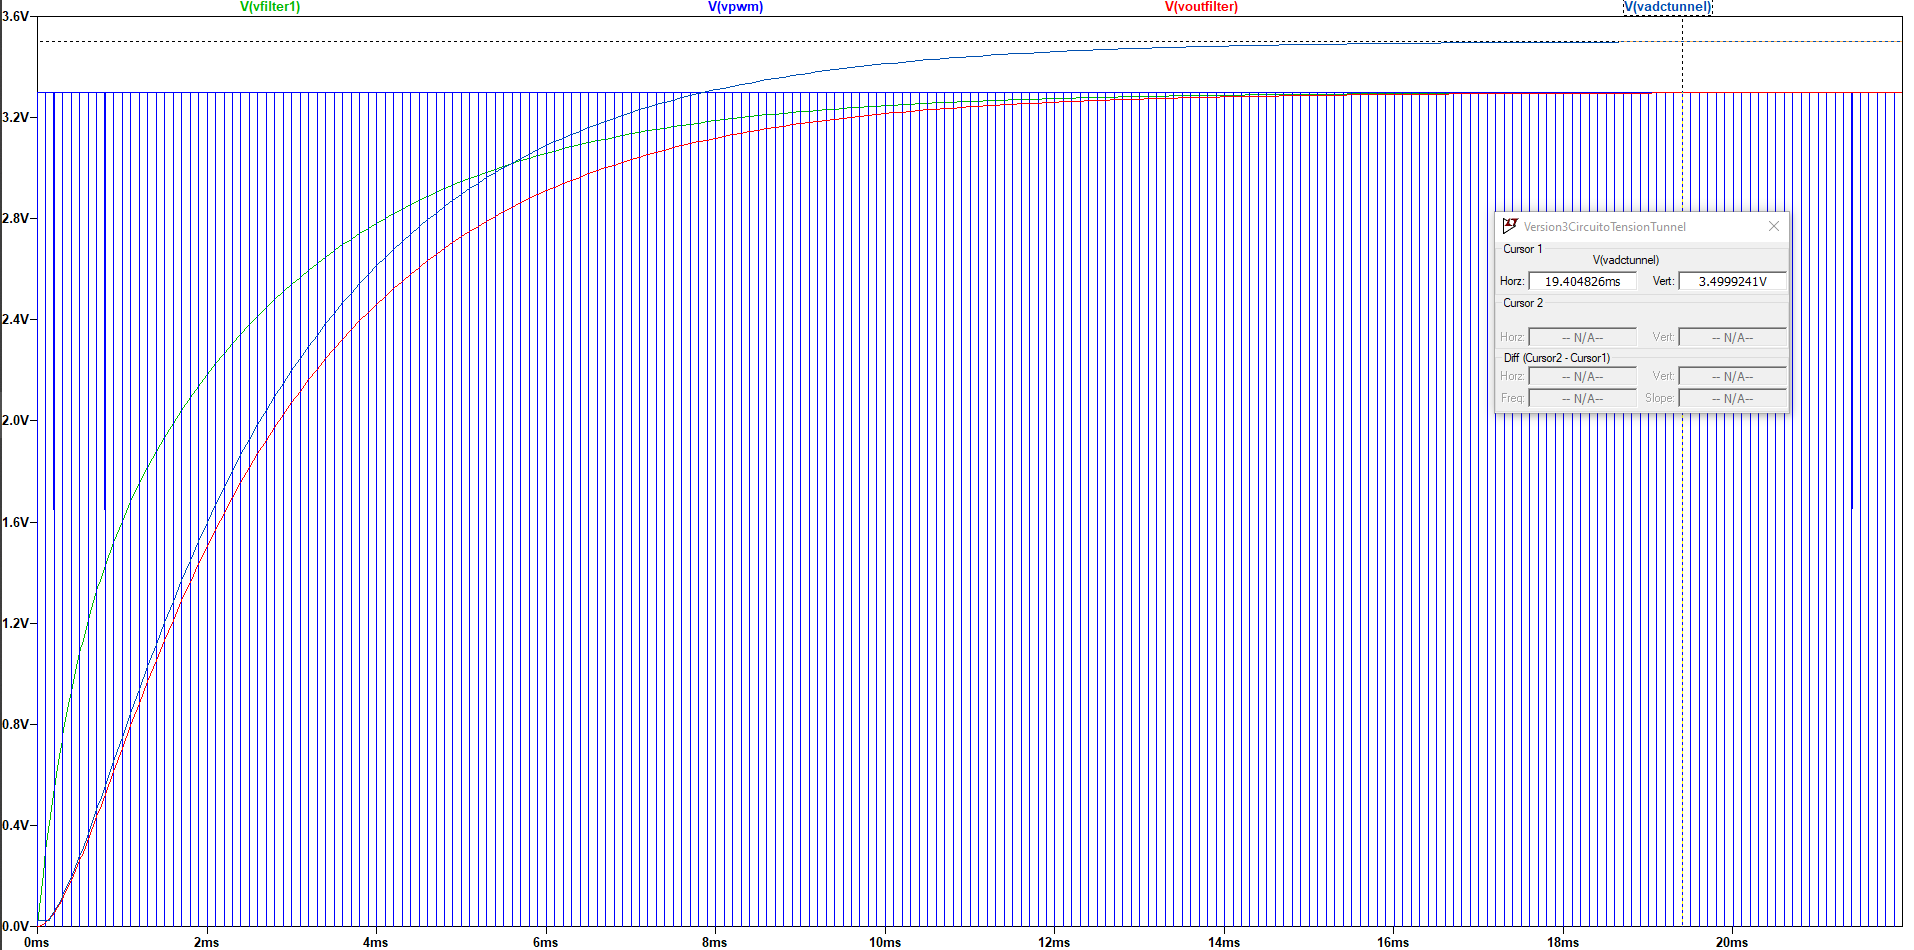
\includegraphics[width=1.1\linewidth]{Figuras/datalogger/Hardware/pwm100Percent.png}
    \caption{Señales simuladas para un ciclo de trabajo al 100 \% de la señal de entrada.}
    \label{fig:pwm100Percent}
\end{figure}
En la simulación, al regular el ciclo de trabajo de la señal de entrada, se obtuvieron distintos niveles de tensión continua. Esto se puede observar en las Figuras \ref{fig:pwm75Percent} y \ref{fig:pwm55Percent}, que muestran los resultados para ciclos de trabajo del $75\%$ y $55\%$, respectivamente.

\begin{figure}[H]
    \centering
    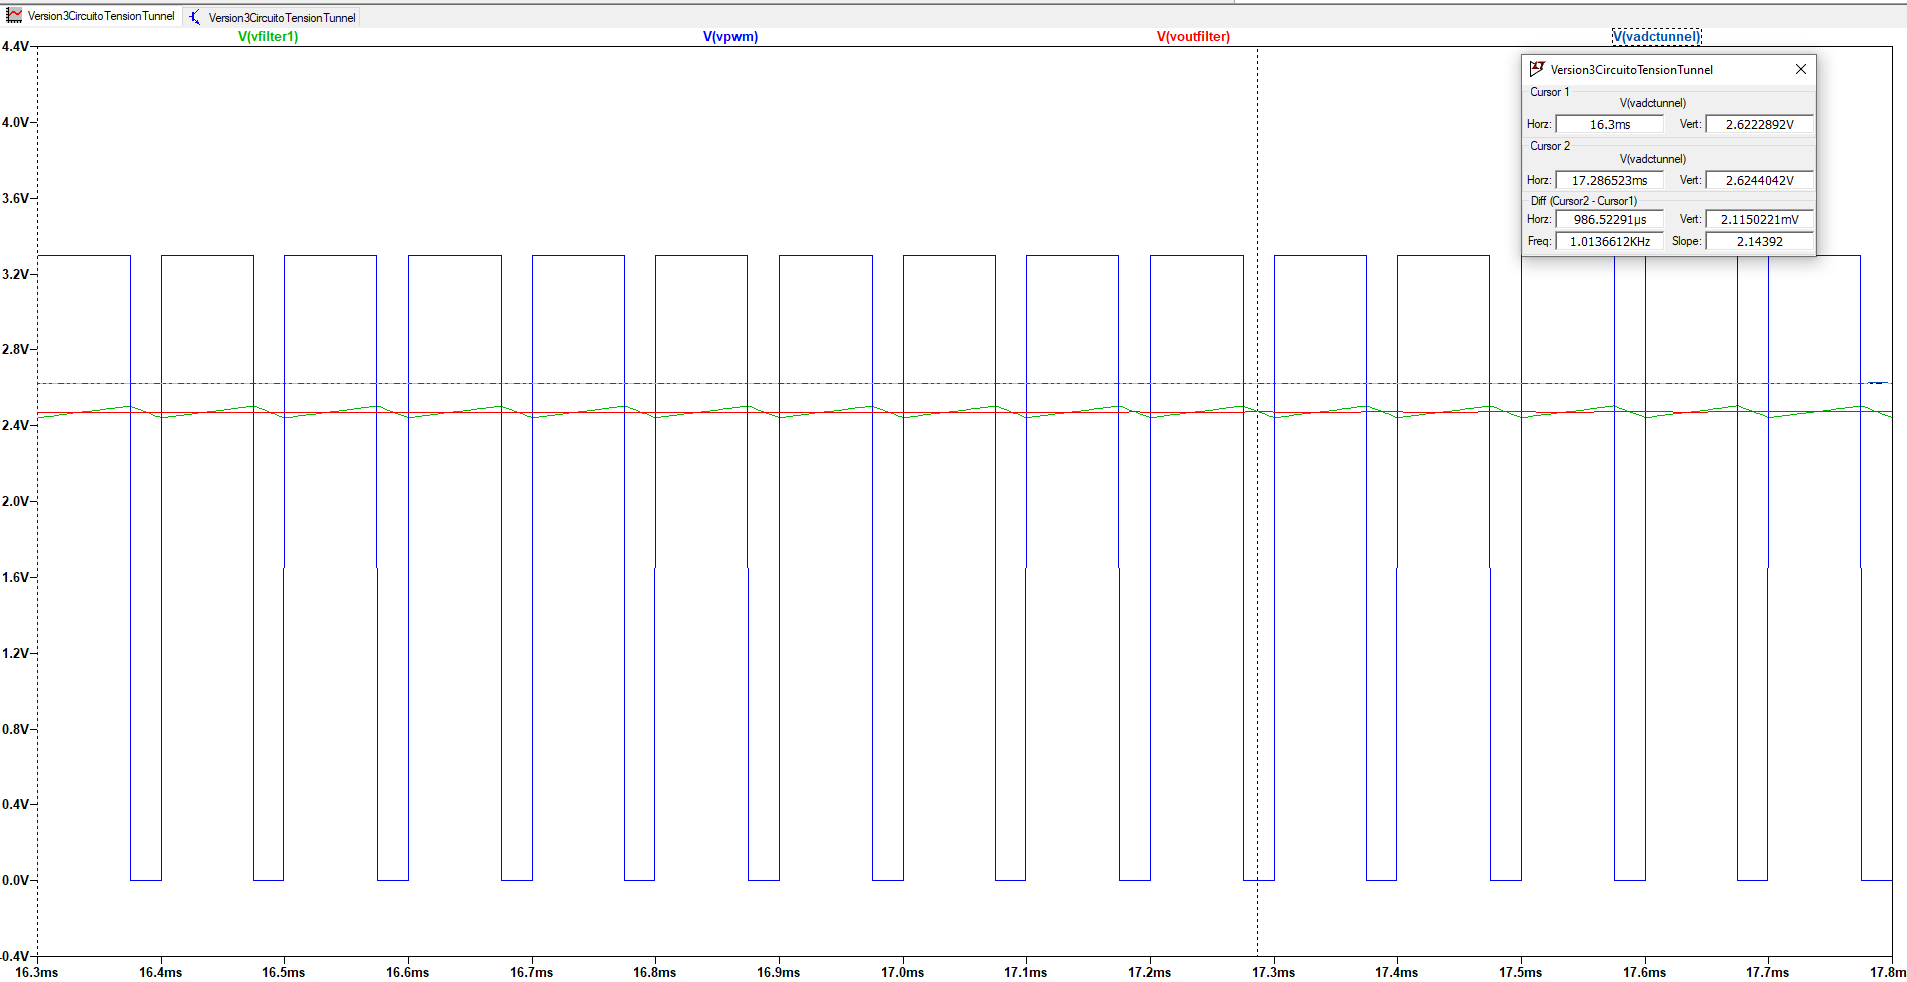
\includegraphics[width=1.1\linewidth]{Figuras/datalogger/Hardware/pwm75Percent.png}
    \caption{Señales simuladas para un ciclo de trabajo al 75 \% de la señal de entrada.}
    \label{fig:pwm75Percent}
\end{figure}



\begin{figure}[H]
    \centering
    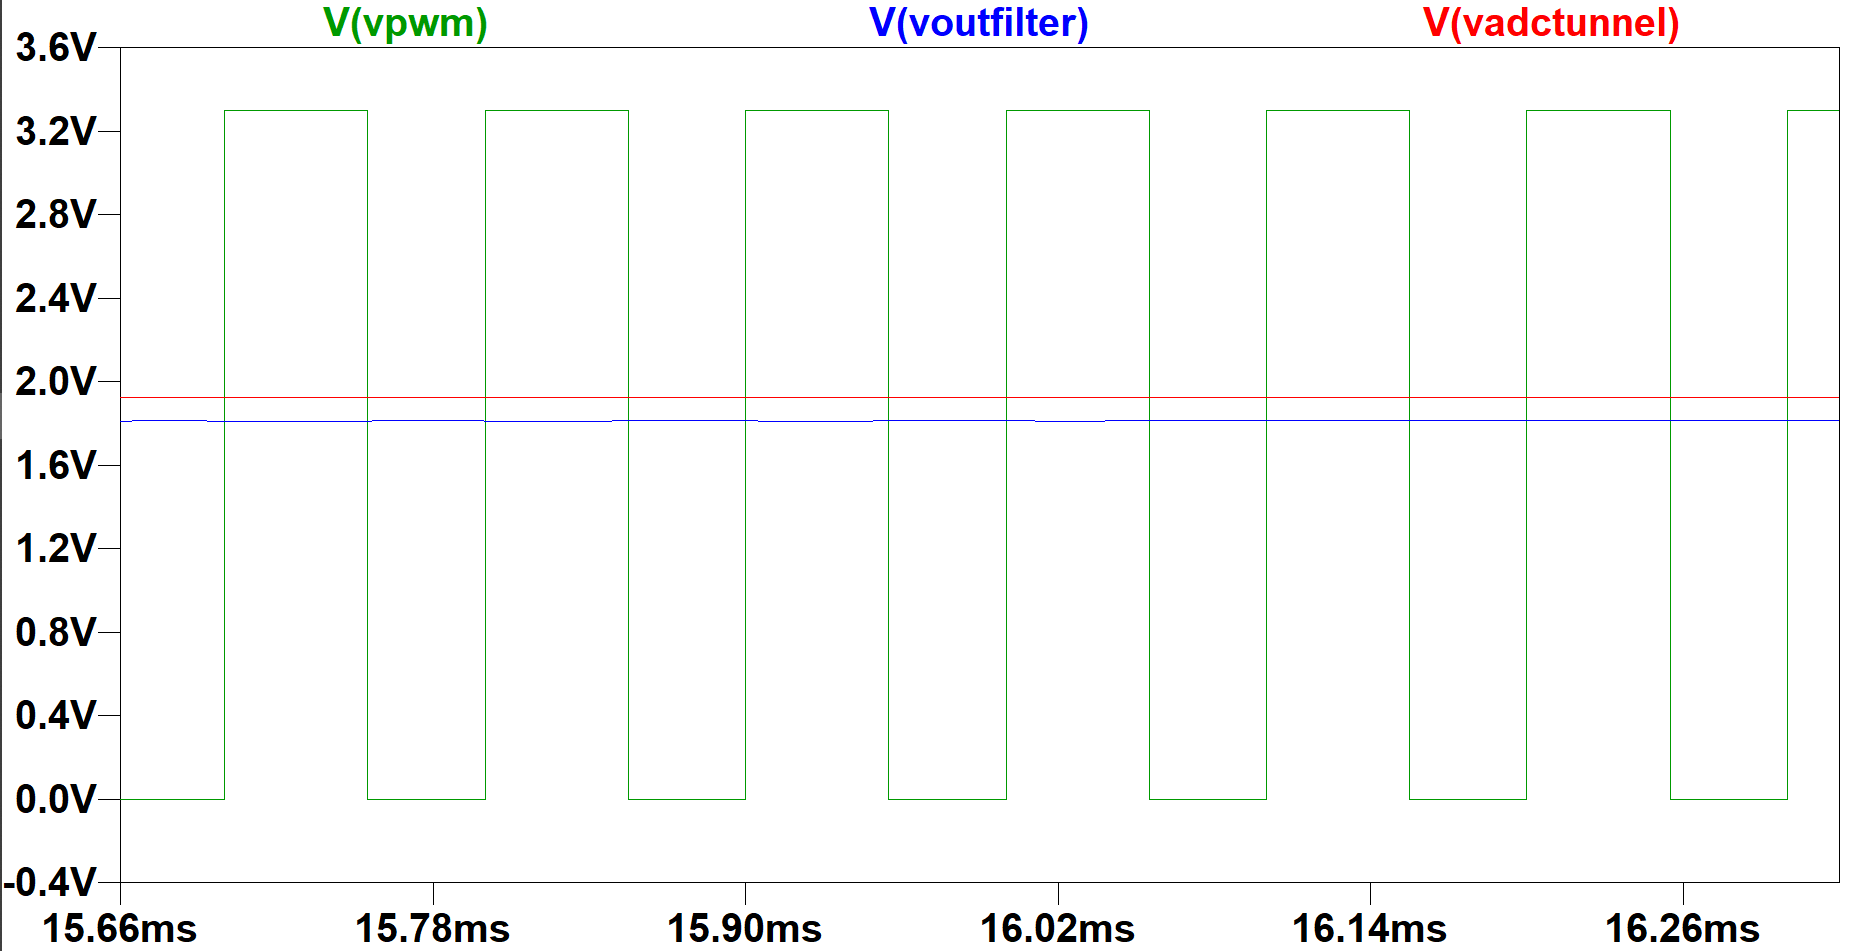
\includegraphics[width=1.1\linewidth]{Figuras/datalogger/Hardware/pwm55Percent.png}
    \caption{Señales simuladas para un ciclo de trabajo al 75 \% de la señal de entrada.}
    \label{fig:pwm55Percent}
\end{figure}


\subsubsection{Implementación del circuito}

Se implementó el circuito de la Figura \ref{fig:esquemPWM} en un protoboard de prueba con componentes Through-Hole Technology (THT), conectado a la EDU-CIAA, como se muestra en la Figura \ref{fig:BancoMedicion1}. Para comprobar y caracterizar el comportamiento del PWM, se utilizaron distintos valores de ciclo de trabajo configurados manualmente en el firmware del microcontrolador. El ciclo de trabajo de la señal cuadrada se modificó desde 1 hasta 255, equivalente a un rango de 0\% a 100\%.

Para realizar estas mediciones, se utilizó un osciloscopio RIGOL DS2302A. En el canal 1 se midió la señal PWM de $\SI{10}{\kilo\hertz}$ con amplitud de $\SI{3.3}{\volt}$ que sale de un pin digital de la placa de desarrollo y se conecta a la entrada al circuito PWM diseñado. En el canal 2 se midió la señal continua a la salida del amplificador operacional (ADCinVariador), ajustando el potenciómetro $RV1$ del esquema de la Figura \ref{fig:esquemPWM}, para obtener $\SI{3.5}{\volt}$ cuando el ciclo de trabajo es $100\%$.

\begin{figure}[H]
    \centering
    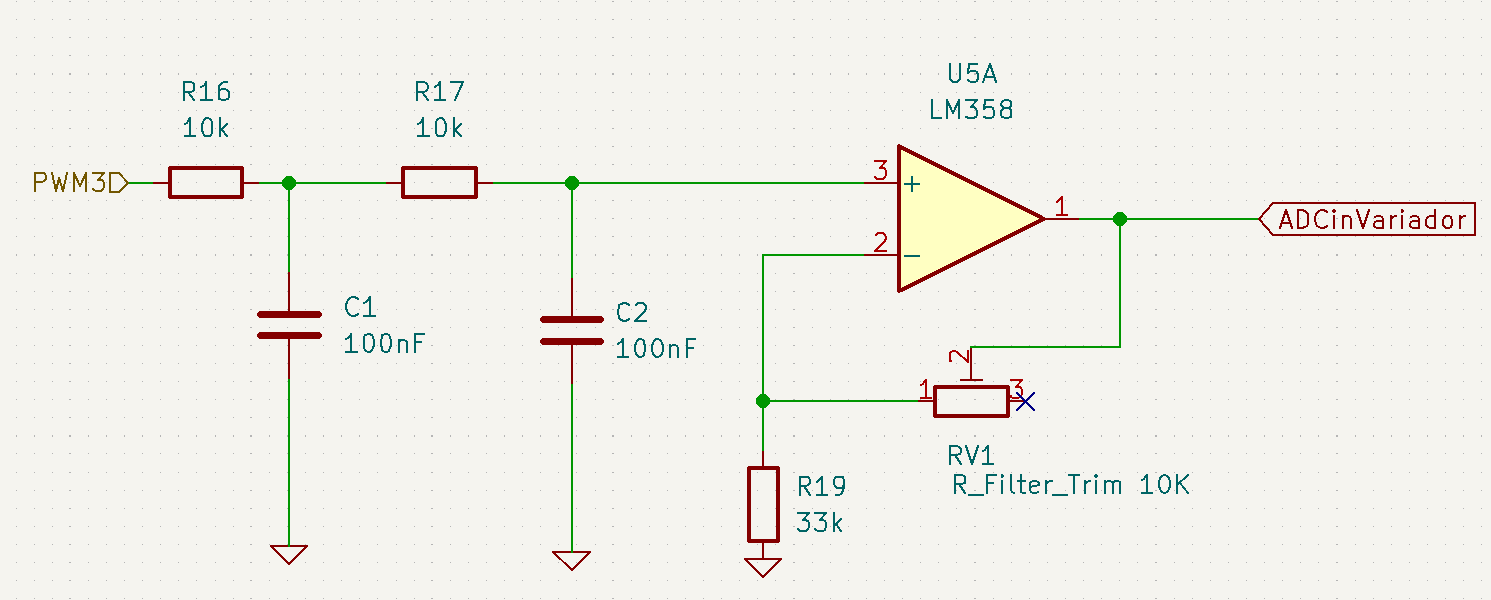
\includegraphics[width=1.1\linewidth]{Figuras/datalogger/Hardware/esquemPWM.png}
    \caption{Esquemático del circuito PWM que controla la velocidad del túnel de viento por programación.}
    \label{fig:esquemPWM}
\end{figure}

\begin{figure}[H]
    \centering
    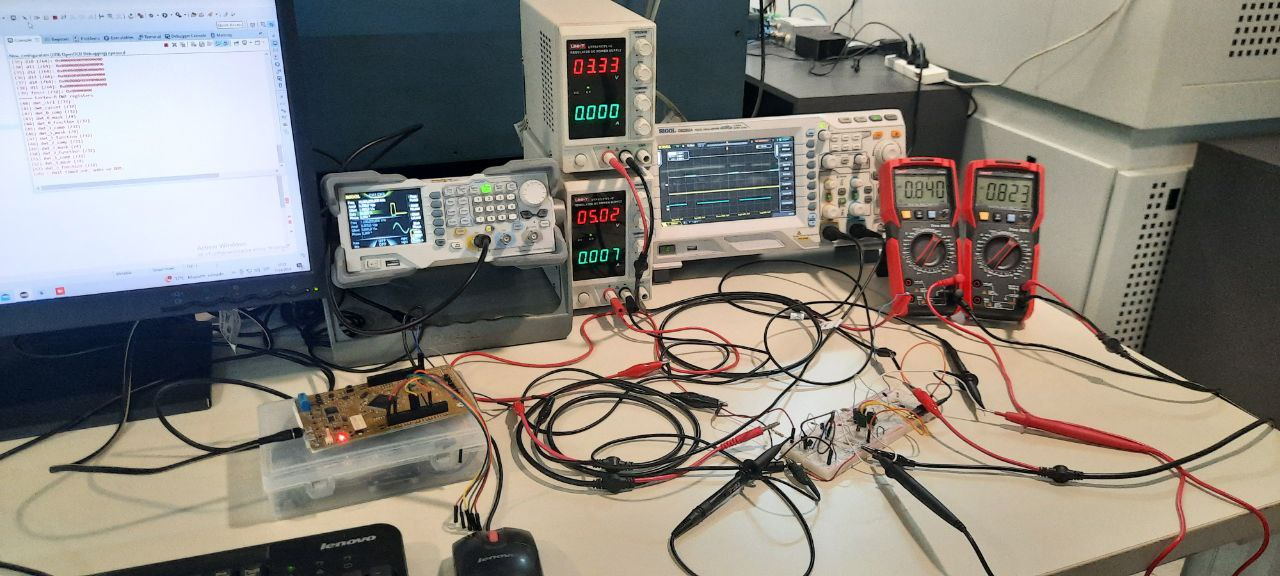
\includegraphics[width=1.1\linewidth]{Figuras/datalogger/Hardware/BancoMedicion1.jpg}
    \caption{Banco de medición para caracterizar el circuito PWM.}
    \label{fig:BancoMedicion1}
\end{figure}

Los resultados de las mediciones realizadas con el osciloscopio se muestran en las Figuras \ref{fig:1}, \ref{fig:63}, \ref{fig:127}, \ref{fig:191} y \ref{fig:255}, equivalente a ciclo de trabajo de 1\%, 25\%, 50\%, 75\% y 100\% respectivamente.



\begin{figure}[H]
    \centering
    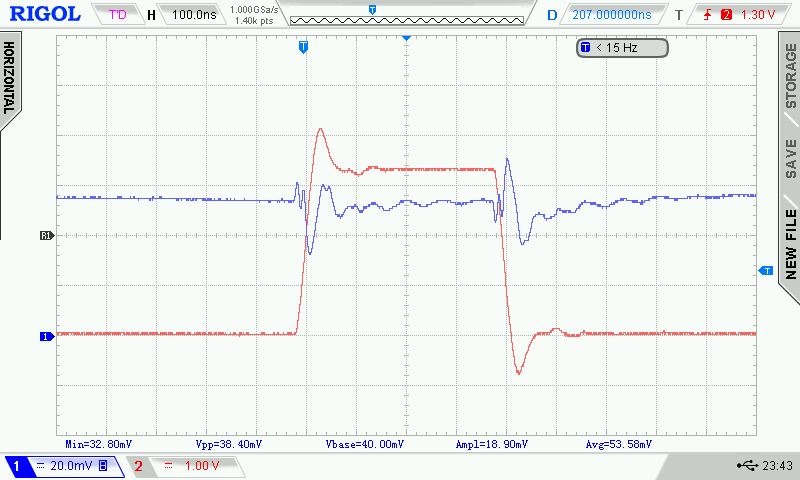
\includegraphics[width=0.9\linewidth]{Figuras/datalogger/Hardware/MedicionesPWM/1.png}
    \caption{Medición de la señal PWM (rojo) con un ciclo de trabajo de (1\%) y la señal continua a la salida del amplificador operacional (azul) iguala $\SI{53.5}{\milli\volt}$.}
    \label{fig:1}
\end{figure}

\begin{figure}[H]
    \centering
    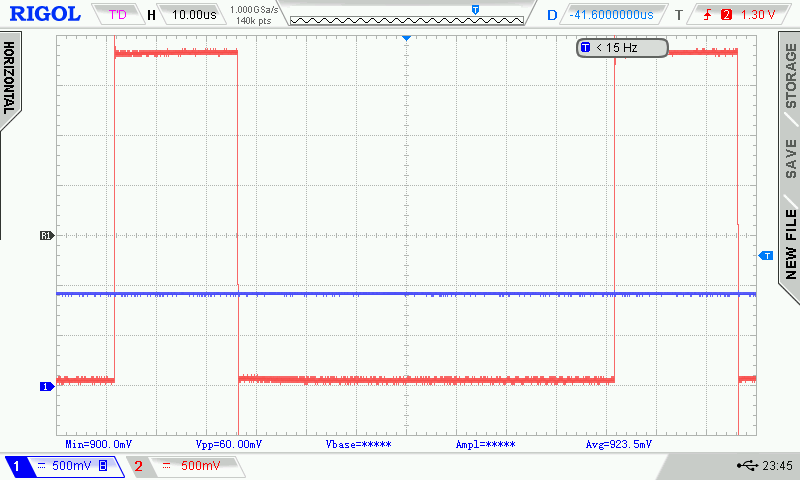
\includegraphics[width=0.9\linewidth]{Figuras/datalogger/Hardware/MedicionesPWM/63.png}
    \caption{Medición de la señal PWM (rojo) con un ciclo de trabajo de (25\%) y la señal continua a la salida del amplificador operacional (azul) iguala $\SI{900}{\milli\volt}$.}
    \label{fig:63}
\end{figure}


\begin{figure}[H]
    \centering
    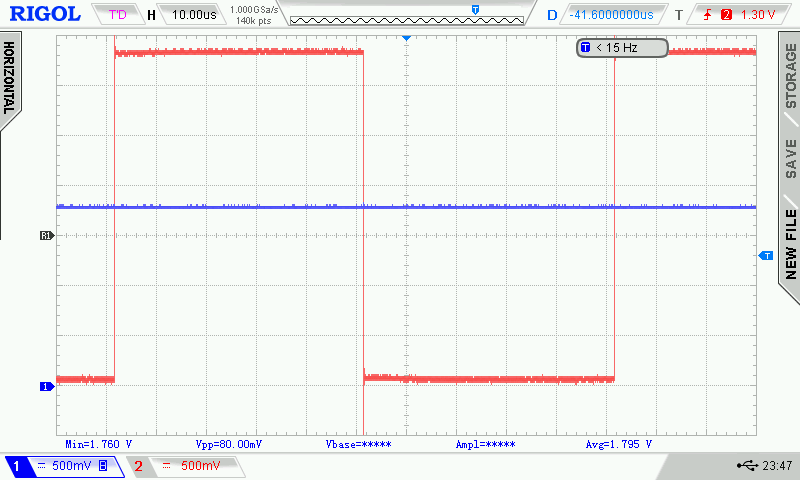
\includegraphics[width=0.9\linewidth]{Figuras/datalogger/Hardware/MedicionesPWM/127.png}
    \caption{Medición de la señal PWM (rojo) con un ciclo de trabajo de (50\%) y la señal continua a la salida del amplificador operacional (azul) iguala $\SI{1.8}{\volt}$. }
    \label{fig:127}
\end{figure}


\begin{figure}[H]
    \centering
    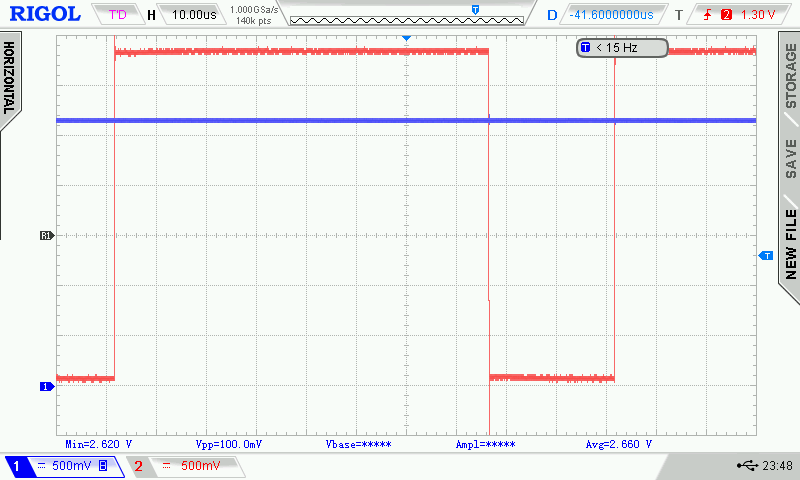
\includegraphics[width=0.9\linewidth]{Figuras/datalogger/Hardware/MedicionesPWM/191.png}
    \caption{Medición de la señal PWM (rojo) con un ciclo de trabajo de (75\%) y la señal continua a la salida del amplificador operacional (azul) iguala $\SI{2.65}{\volt}$.}
    \label{fig:191}
\end{figure}


\begin{figure}[H]
    \centering
    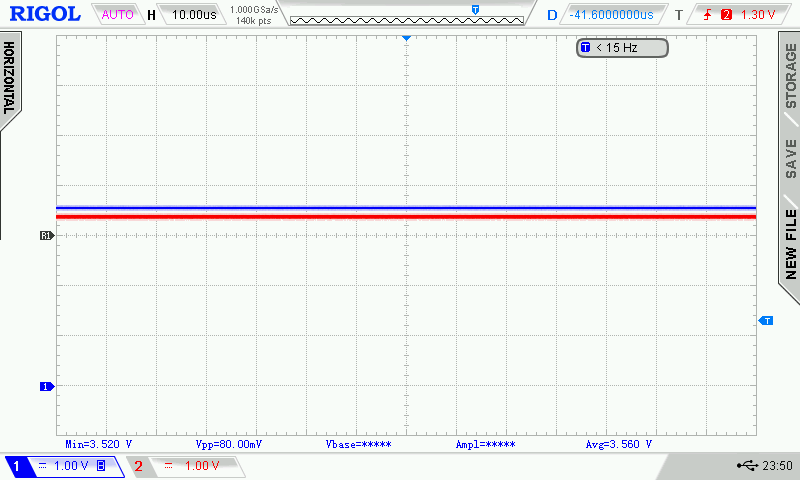
\includegraphics[width=0.9\linewidth]{Figuras/datalogger/Hardware/MedicionesPWM/255.png}
    \caption{Medición de la señal PWM (rojo) con un ciclo de trabajo de (100\%) y la señal continua a la salida del amplificador operacional (azul) iguala $\SI{3.56}{\volt}$.}
    \label{fig:255}
\end{figure}
Luego de caracterizar el circuito PWM, se lo llevó al túnel de viento y se conectó la tensión de la salida del operacional al pin de entrada $VADC$ del variador de velocidad. A continuación, se realizó un barrido del ciclo de trabajo desde 0 hasta 255 (0\% a 100\%), midiendo con un voltímetro, UNI-T modelo UT89X, la tensión entregada al túnel y, con el anemómetro VAISALA WMT700 dentro del túnel, la velocidad en metros por segundo obtenida para cada ciclo de trabajo. En la tabla \ref{tab:windSpeedDataAsc} se muestran los resultados de un barrido ascendente, y en la tabla \ref{tab:windSpeedDataDesc}, los resultados de un barrido descendente.

\begin{table}[H]
\centering
\begin{tblr}{
  cells = {c},
  row{1} = {Sail},
  hlines,
  vlines,
}
{\textbf{Ciclo de trabajo}\\\textbf{[0 - 255]}} & \textbf{VadcTunnel [\unit{\milli\volt}]} & \textbf{Viento [\unit{\meter\per\second}]} \\
0                                                & 4.2                      & 1                     \\
1                                                & 16.6                     & 1.1                   \\
2                                                & 30.3                     & 1.2                   \\
31                                               & 427                      & 4.5                   \\
63                                               & 864                      & 7.8                   \\
94                                               & 1291                     & 11.1                  \\
127                                              & 1745                     & 14.7                  \\
158                                              & 2170                     & 18                    \\
191                                              & 2621                     & 21.5                  \\
222                                              & 3048                     & 24.5                  \\
255                                              & 3500                     & 26.3                  
\end{tblr}
\caption{Mediciones para ciclos de trabajo en modo Ascendente, VadcTunnel y la velocidad del viento.}
\label{tab:windSpeedDataAsc}
\end{table}



\begin{table}[H]
\centering
\begin{tblr}{
  cells = {c},
  row{1} = {Sail},
  hlines,
  vlines,
}
{\textbf{Ciclo de trabajo}\\\textbf{[0 - 255]}} & \textbf{VadcTunnel [\unit{\milli\volt}]} & \textbf{Viento [\unit{\meter\per\second}]} \\
255                               & 3501                     & 25.9                  \\
222                               & 3048                     & 24.5                  \\
191                               & 2622                     & 21.3                  \\
158                               & 2170                     & 18                    \\
127                               & 1744                     & 14.7                  \\
94                                & 1291                     & 11.1                  \\
63                                & 865                      & 7.8                   \\
31                                & 426                      & 4.5                   \\
2                                 & 30                       & 1.3                   \\
1                                 & 16                       & 1.1                   \\
0                                 & 4                        & 1.0                   
\end{tblr}
\caption{Mediciones para ciclos de trabajo en modo Descendente, VadcTunnel y la velocidad del viento.}
\label{tab:windSpeedDataDesc}
\end{table}

A partir de los resultados obtenidos para el ciclo de trabajo versus la tensión en el variador y el ciclo de trabajo versus la velocidad del viento medida con el anemómetro, se determina una velocidad máxima de viento de $\SI{26}{\meter\per\second}$ para una tensión de $\SI{3.5}{\volt}$. Además, dado que se tienen 255 niveles de tensión, se obtiene una resolución en tensión de $\frac{\SI{3.5}{\volt}}{255} = \SI{13.7}{\milli\volt}$ y una resolución en velocidad del viento de $\frac{\SI{26}{\meter\per\second}}{255} = \SI{0.101}{\meter\per\second}$. Con estas mediciones y la caracterización del circuito PWM, este quedó listo para ser integrado en un PCB. Este circuito será la interfaz electrónica para un controlador PID, el cual se explica en la sección \ref{sec:sistemaDeControlPid}.


% \subsubsection{Caracterizacion en el tunel de viento}
% Aca poner las mediciones y pruebas que se hicieron en el tunel, las tablas de Click up
%%%%%%%%%%%%%%%%%%%%%%%%%%%%%%%%%%%%%%%%%%%%%%%%%%%%%%%%%%%%%%%%%%%%%%%%%%%%%%%%%%%%%%%%%%%%%%%%%%%%%%%
\subsection{Circuito de adquisición de tensión del variador}\label{sec:adquisicionVadcTunel}

En esta sección se diseñó un circuito que permite tomar muestras de la tensión entregada al variador del túnel de viento. El circuito funciona como un voltímetro que mide la tensión instantánea y la envía a un canal analógico-digital (ADC\_CH2) de la EDU-CIAA. 

Debido a que la señal de continua, para un ciclo de trabajo del 100\%, es de $\SI{3.5}{\volt}$, fue necesario adaptar esta señal a $\SI{3.3}{\volt}$, ya que esta es la tensión máxima de entrada para los canales ADC de la EDU-CIAA.

\subsubsection{Simulación del circuito}

En la Figura \ref{fig:adcCiaaCircuitSimulate} se muestra el diseño del circuito, la señal de continua $\text{VadcTunnel}$ se conecta al segundo operacional del chip LM358, en modo seguidor para adaptar la impedancia y no cargar a la etapa anterior, luego a la salida del operacional se conecta un divisor de tensión para adaptar la tensión a $\SI{3.3}{\volt}$, además se agrega una etapa de protección con dos diodos conectados entre la fuente de $\SI{3.3}{\volt}$ y GND para limitar el voltaje en caso de que la tensión a la salida del operacional sea superior a la fuente. Finalmente, se pone una resistencia de $\SI{1}{\kilo\ohm}$ para limitar la corriente en  $\text{VadcCIAA}$.

\begin{figure}[H]
    \centering
    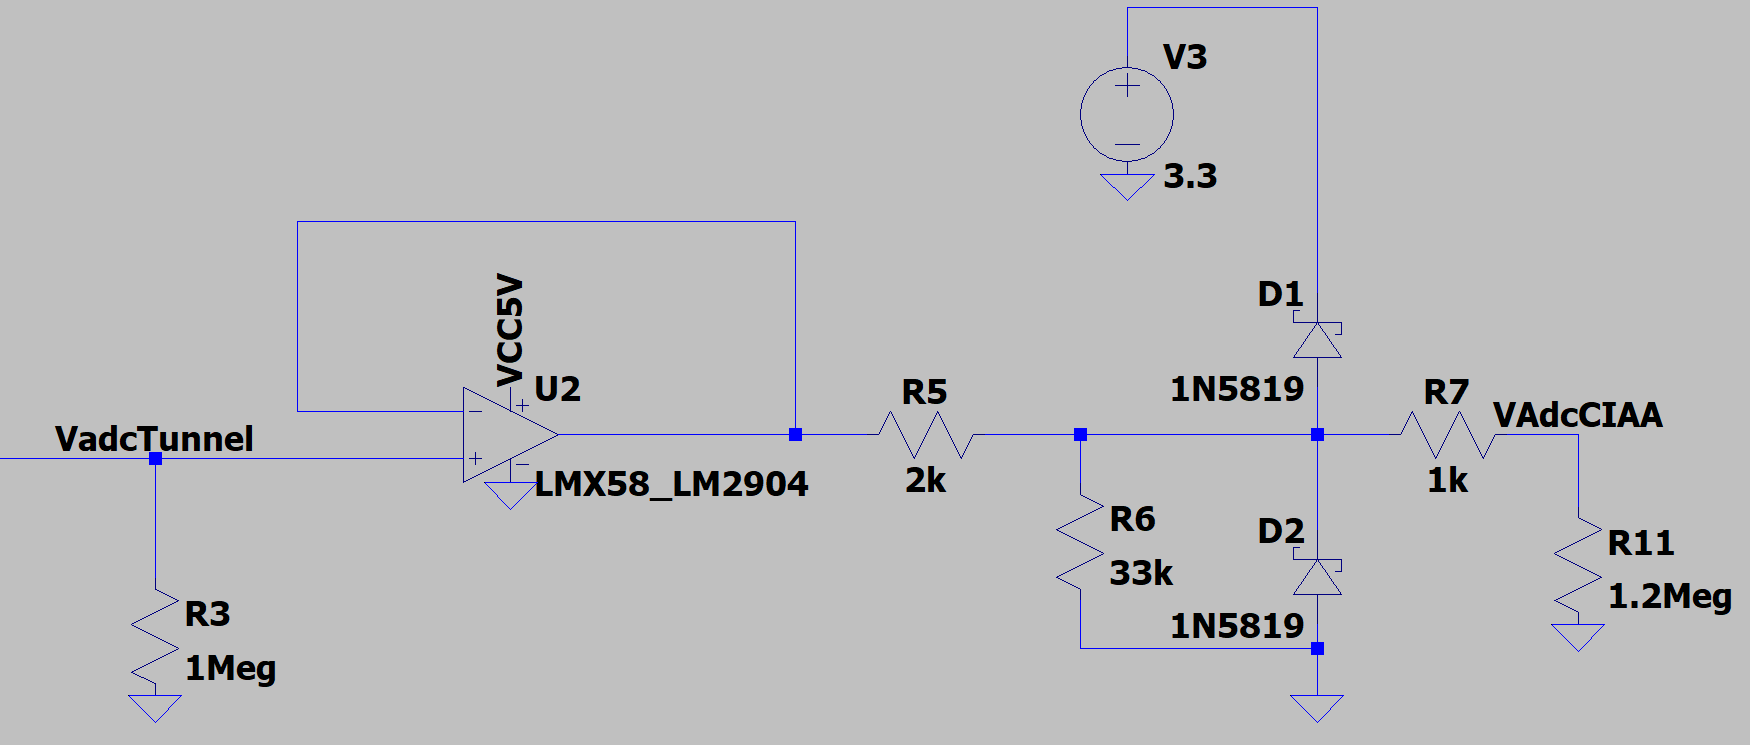
\includegraphics[width=1.1\linewidth]{Figuras/datalogger/Hardware/adcCiaaCircuitSimulate.png}
    \caption{Circuito diseñado para tomar muestras de la señal que se suministra al variador de velocidad y se las envía a una canal analógico-digital de la EDU-CIAA.}
    \label{fig:adcCiaaCircuitSimulate}
\end{figure}
Los resultados de la simulación del circuito descrito se muestran en la Figura \ref{fig:adc100PercentPwm} para un ciclo de trabajo del $100\%$ y en la Figura \ref{fig:adc55PercentPwm} para un ciclo de trabajo del $55\%$. En ambos casos, se puede apreciar que la señal $\text{vadcCIAA}$ (azul) está por debajo de la señal $\text{vadcTunel}$ (verde), lo cual garantiza que no se superen los $\SI{3.3}{\volt}$ a la entrada del pin analógico-digital de la placa de desarrollo.


\begin{figure}[H]
    \centering
    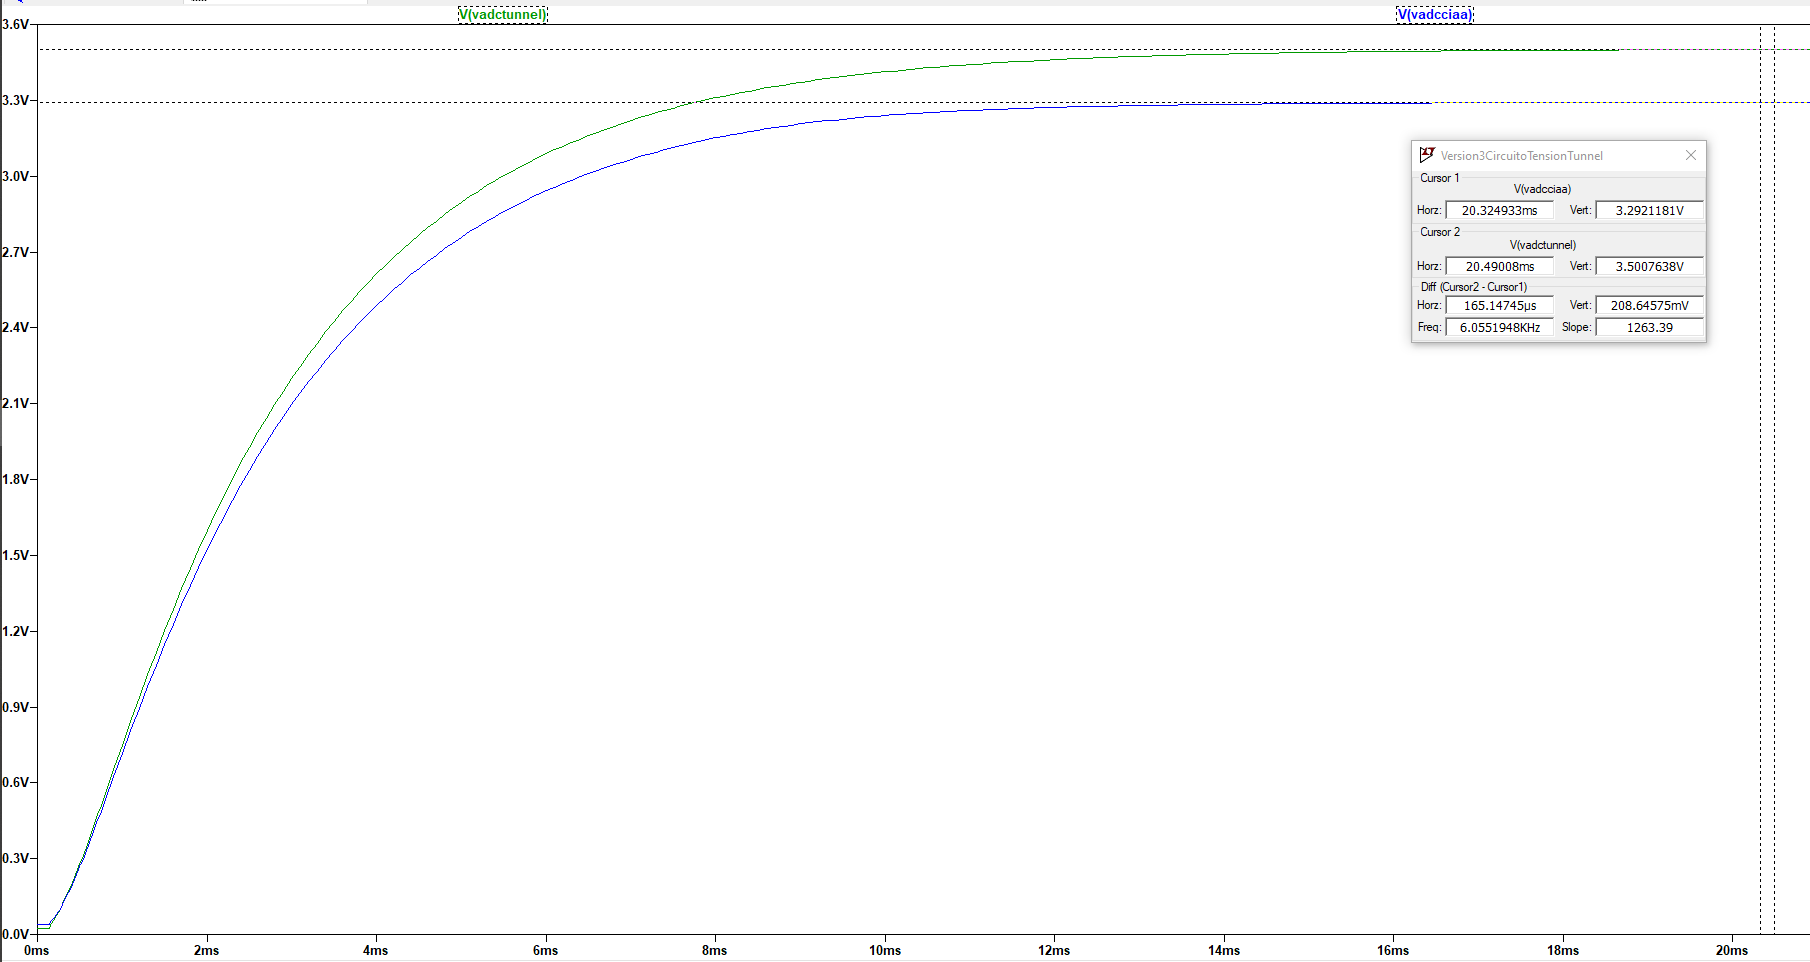
\includegraphics[width=1.1\linewidth]{Figuras/datalogger/Hardware/adc100PercentPwm.png}
    \caption{Señales simuladas a la salida del variador de velocidad y a la entrada del pin analógico-digital de la EDU-CIAA para un ciclo de trabajo del 100\%.}
    \label{fig:adc100PercentPwm}
\end{figure}

\begin{figure}[H]
    \centering
    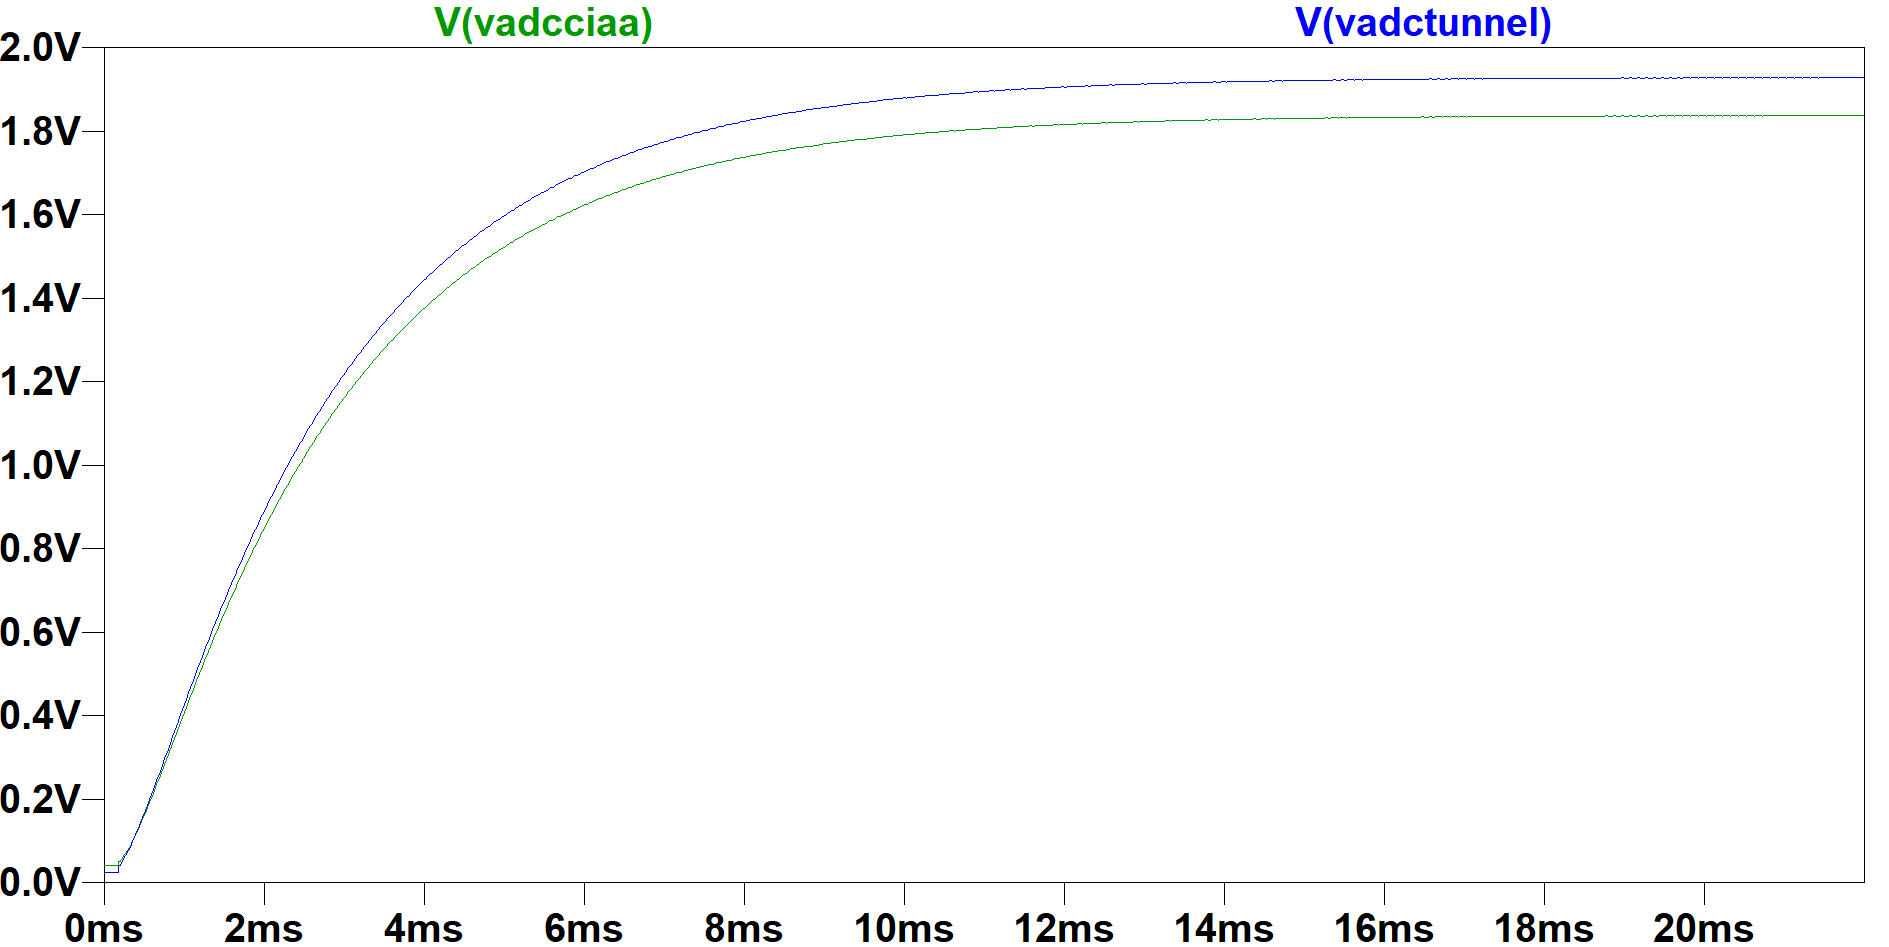
\includegraphics[width=1.1\linewidth]{Figuras/datalogger/Hardware/adc55PercentPwm.png}
    \caption{Señales simuladas a la salida del variador de velocidad y a la entrada del pin analógico-digital de la EDU-CIAA para un ciclo de trabajo del 55\%.}
    \label{fig:adc55PercentPwm}
\end{figure}

\subsubsection{Implementación del circuito}

Se implementó el circuito de la Figura \ref{fig:esquemADCTunel}. Para ajustar los niveles de tensión de $\SI{3.5}{\volt}$ a $\SI{3.3}{\volt}$, se agregó en el divisor de tensión, un resistor variable (trimmer) de RV2 = $\SI{10}{\kilo\ohm}$. Luego se conectó los diodos a la fuente de $\SI{3.3}{\volt}$ de la EDU-CIAA y se agregó un la resistencia limitadora de tensión de $R18 = \SI{1}{\kilo\ohm}$, esta señal de continua se muestrea con una resolución  de $\frac{\SI{3.3}{\volt}}{1024} = \SI{3.22}{\milli\volt}$  en el canal ADC\_CH2 de la placa de desarrollo.

\begin{figure}[H]
    \centering
    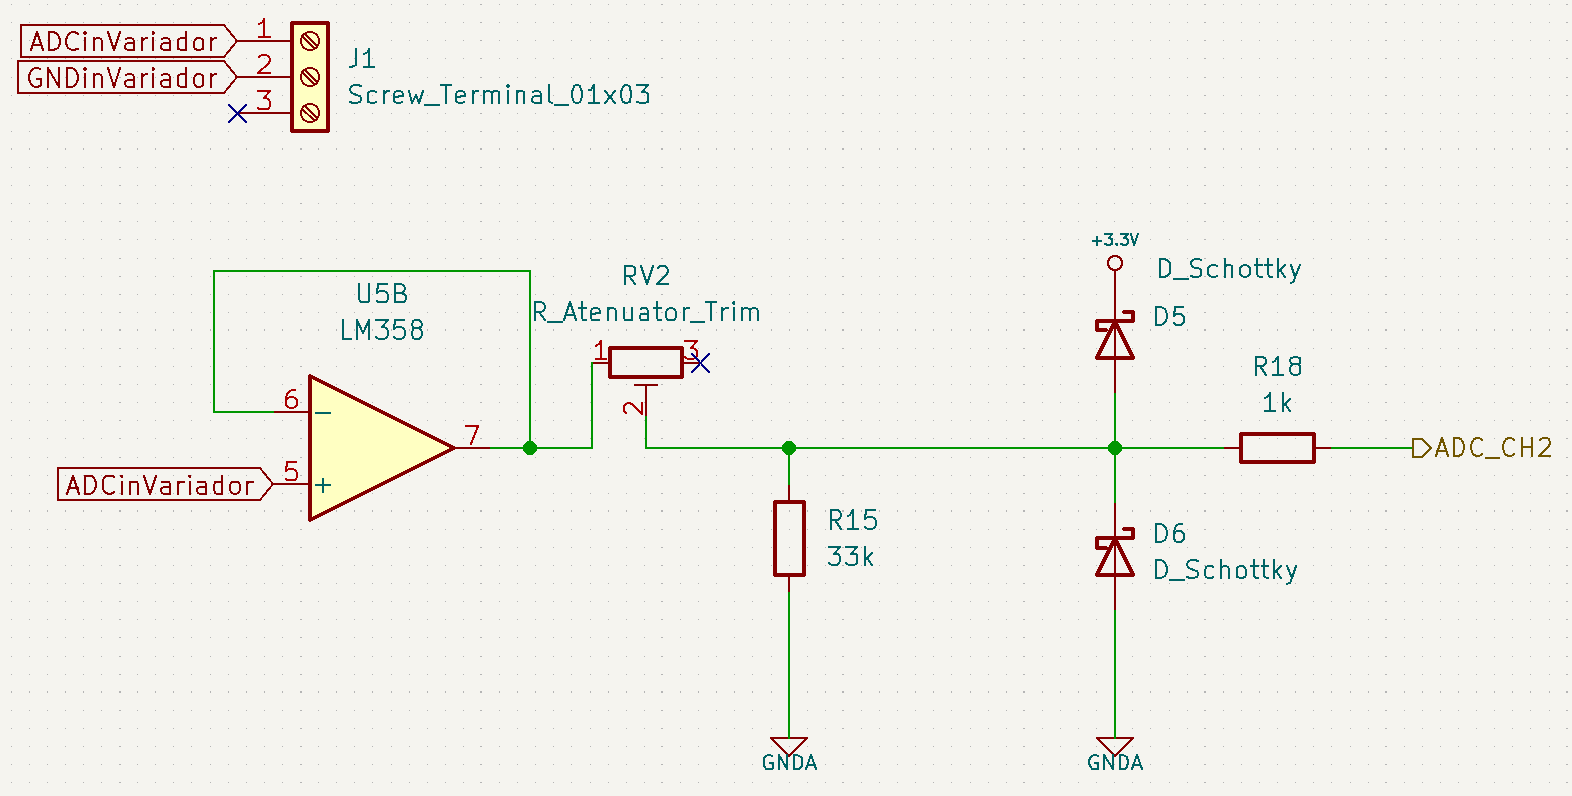
\includegraphics[width=1.1\linewidth]{Figuras/datalogger/Hardware/esquemADCTunel.png}
    \caption{Esquemático de la implementación del circuito que toma muestras de la señal continua que ingresa al variador de velocidad.}
    \label{fig:esquemADCTunel}
\end{figure}

Se conectó dos voltímetros, uno en la señal de entrada del variador y otro en la señal que ingresa al ADC de la EDU-CIAA, los resultados de estas mediciones se observan en las tablas \ref{tab:medicionesVadcCIAA_ascendente} para un barrido ascendente y \ref{tab:medicionesVadcCIAA_descendente} para un barrido descendente.
\begin{table}[H]
\centering
\begin{tblr}{
  cells = {c},
  row{1} = {Sail},
  hlines,
  vlines,
}
{\textbf{Ciclo de trabajo }\\\textbf{[0 - 255]}} & \textbf{VadcTunnel [\unit{\milli\volt}]} & \textbf{VadcCIAA [\unit{\milli\volt}]} \\
0                                                & 4.2                      & 20                        \\
1                                                & 16.6                     & 16.7                      \\
2                                                & 30.3                     & 37.3                      \\
31                                               & 427                      & 421.3                     \\
63                                               & 864                      & 856                       \\
94                                               & 1291                     & 1280                      \\
127                                              & 1745                     & 1725                      \\
158                                              & 2170                     & 2146                      \\
191                                              & 2621                     & 2593                      \\
222                                              & 3048                     & 3013                      \\
255                                              & 3500                     & 3364                      
\end{tblr}
\caption{Mediciones a la entrada pin $VADC$ del variador y en el pin ADC\_CH2 de la EDU-CIAA, para un barrido ascendente  del ciclo de trabajo.}
\label{tab:medicionesVadcCIAA_ascendente}
\end{table}



\begin{table}[H]
\centering
\begin{tblr}{
  cells = {c},
  row{1} = {Sail},
  hlines,
  vlines,
}
{\textbf{Ciclo de trabajo }\\\textbf{[0 - 255]}} & \textbf{VadcTunnel [\unit{\milli\volt}]} & \textbf{VadcCIAA [\unit{\milli\volt}]} \\
255                                              & 3501                     & 3364                    \\
222                                              & 3048                     & 3012                    \\
191                                              & 2622                     & 2593                    \\
158                                              & 2170                     & 2146                    \\
127                                              & 1744                     & 1725                    \\
94                                               & 1291                     & 1277                    \\
63                                               & 865                      & 855                     \\
31                                               & 426                      & 422                     \\
2                                                & 30                       & 38                      \\
1                                                & 16                       & 27                      \\
0                                                & 4                        & 21                      
\end{tblr}
\caption{Mediciones a la entrada pin $VADC$ del variador y en el pin ADC\_CH2 de la EDU-CIAA, para un barrido descendente del ciclo de trabajo.}
\label{tab:medicionesVadcCIAA_descendente}
\end{table}
Este circuito permite monitorear por software los niveles de tensión que estamos entregando al variador de velocidad y su correspondiente ciclo de trabajo.

%%%%%%%%%%%%%%%%%%%%%%%%%%%%%%%%%%%%%%%%%%%%%%%%%%%%%%%%%%%%%%%%%%%%%%%%%%%%%%%%%%%%%%%%%%%%%%%%%%%%%%%
\subsection{Circuito de LEDs indicadores}
Se diseñó el circuito de la Figura \ref{fig:esquemLedsSensor}  para encender y apagar LEDs como indicadores de la recepción de datos de los anemómetros patrón y bajo calibración. Se utilizaron dos LEDs de colores diferentes: uno verde y otro amarillo. El LED verde se asoció al canal RS-485-1 y el LED amarillo al canal RS-485-2.

Cada circuito permite que el LED correspondiente parpadee cada vez que se recibe un dato del anemómetro, con un intervalo predeterminado por software. Si el LED no parpadea, indica que el anemómetro no está enviando datos. Por el contrario, si el LED parpadea, confirma la recepción de datos del anemómetro.

El diseño de cada circuito incluye un transistor NPN y dos resistencias, conectados a un diodo LED. La señal de entrada llega al resistor $ R_4 = \SI{1}{\kilo\ohm} $, el cual está conectado a la base del transistor. El colector del transistor está conectado a una fuente de $\SI{5}{\volt} $, mientras que el emisor está conectado a una resistencia limitadora de corriente $ R5 = \SI{39}{\ohm}$ y luego al ánodo del LED, con su cátodo a masa. Ambos circuitos son prácticamente idénticos, diferenciándose únicamente en los colores de los LEDs y los canales RS-485 a los que están conectados.

\begin{figure}[H]
    \centering
    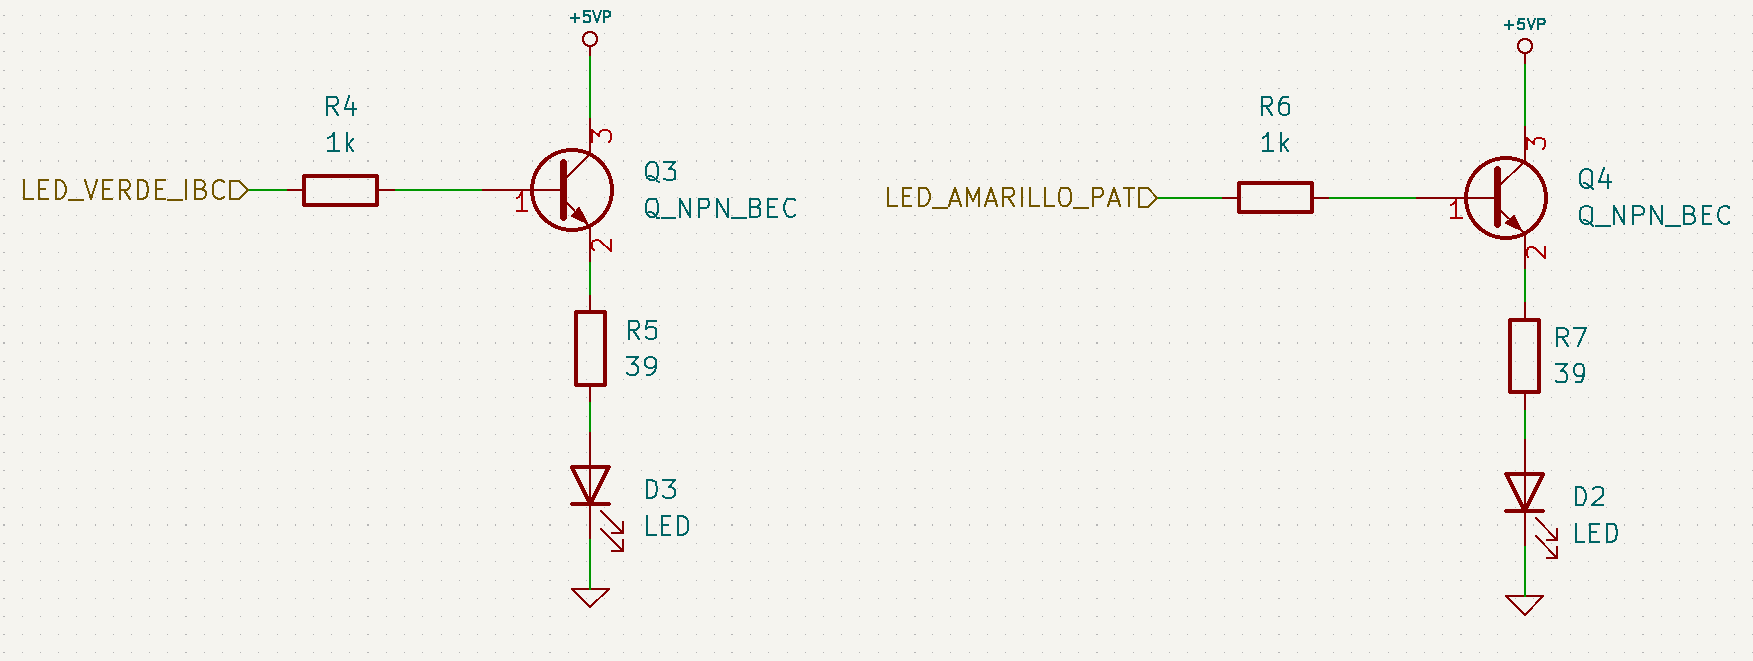
\includegraphics[width=0.95\linewidth]{Figuras/datalogger/Hardware/esquemLedsSensor.png}
    \caption{Esquemático de los circuitos que encienden y apagan dos LEDs, verde y amarillo, cada vez que se recibe un dato de los anemómetros, tanto del patrón como del que está bajo calibración.}

    \label{fig:esquemLedsSensor}
\end{figure}

En La Figura \ref{fig:esquemLedStatusSocket} se muestra un circuito similar al previamente descrito, en el que se utiliza un LED dual como indicador de la conectividad del sistema de la placa de desarrollo con el servidor Websocket descrito en la sección \ref{sec:back_end}. El LED dual se enciende en rojo cuando el sistema de la placa de desarrollo está desconectado del servidor. Al establecerse la conexión a través de Ethernet, el LED cambia a verde. Este cambio de color ocurre automáticamente según el estado de la conectividad con el servidor. El LED dual tiene tres pines: dos ánodos y un cátodo común conectado a masa. Los ánodos están conectados a circuitos que controlan el encendido y apagado del LED según las señales de los pines digitales de la placa de desarrollo.

\begin{figure}[H]
    \centering
    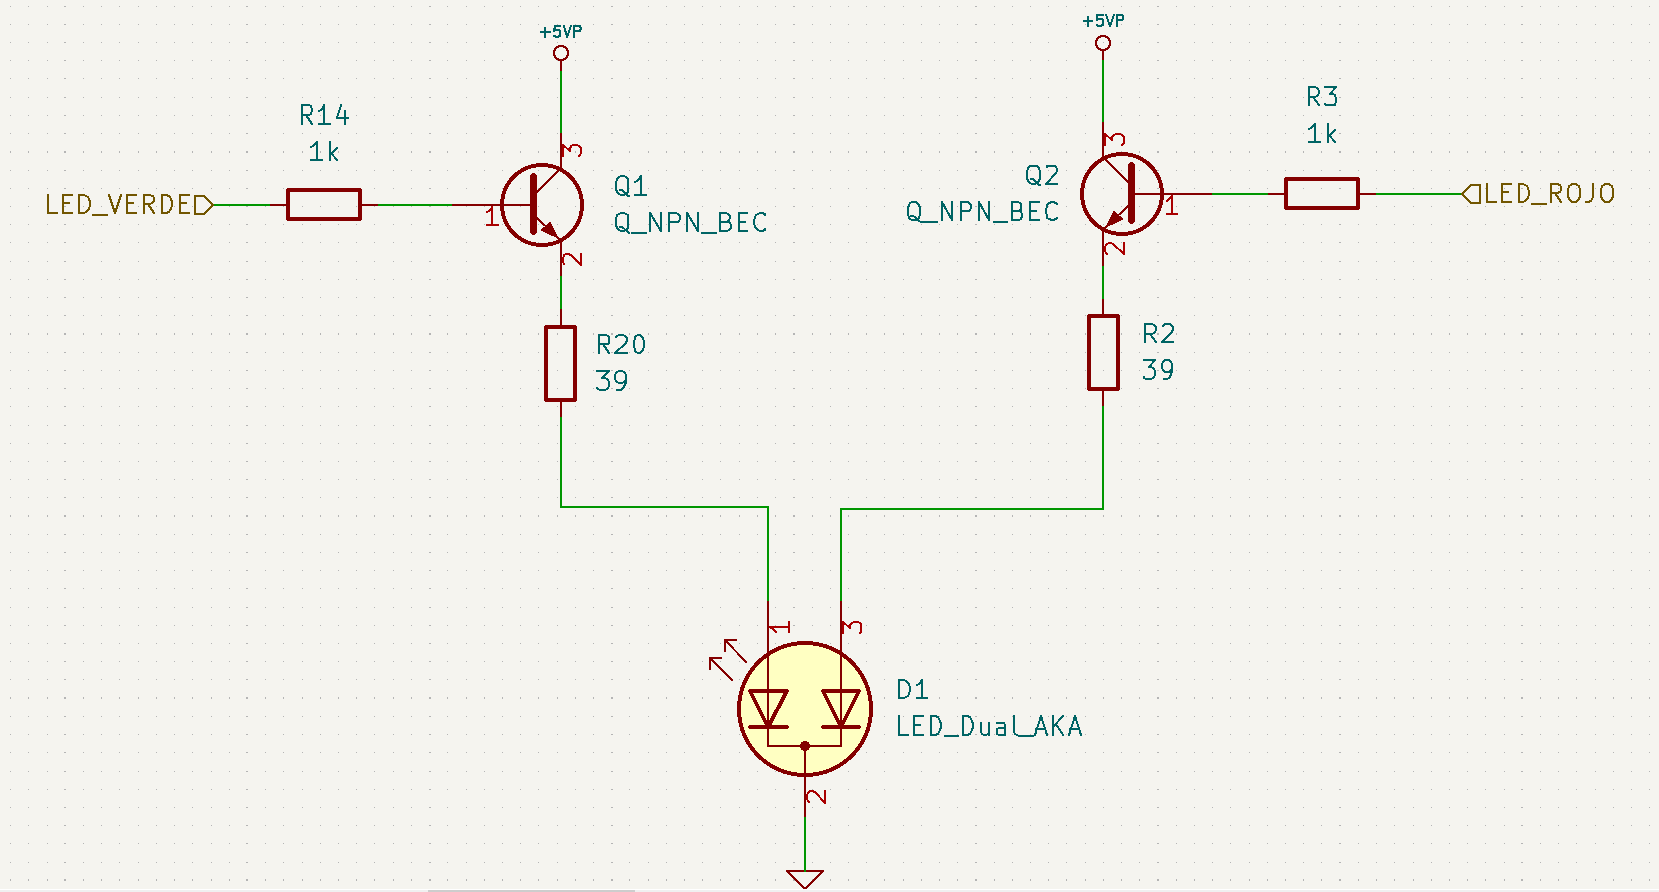
\includegraphics[width=0.95\linewidth]{Figuras/datalogger/Hardware/esquemLedStatusSocket.png}
    \caption{Esquemático del circuito de un LED dual que se enciende en rojo cuando el sistema no está conectado al servidor Websocket y en verde cuando hay una conexión estable con el servidor.}
    \label{fig:esquemLedStatusSocket}
\end{figure}

%%%%%%%%%%%%%%%%%%%%%%%%%%%%%%%%%%%%%%%%%%%%%%%%%%%%%%%%%%%%%%%%%%%%%%%%%%%%%%%%%%%%%%%%%%%%%%%%%%%%%%%


\section{Diseño y construcción del PCB}

En las secciones anteriores se ha descrito el diseño y funcionamiento electrónico de los distintos módulos y circuitos que forman parte del datalogger. Para integrar todo en un solo lugar, se diseñó un shield (poncho) que se conecta sobre la EDU-CIAA. Para ello, se trabajó con la lista de templates que ofrece el proyecto CIAA \cite{CIAA_Ponchos}. Este template tiene un diseño acorde con las dimensiones de la placa EDU-CIAA.

Para el desarrollo del PCB, se utilizó el software KiCad. Primero se cargó el template de la Figura \ref{fig:HojaTemplatePonchoCiaa} que incluye una hoja jerárquica con los pines disponibles en los conectores P1 y P2 y luego se agregó etiquetas jerárquicas por cada pin utilizado en este desarrollo.

\begin{figure}[H]
    \centering
    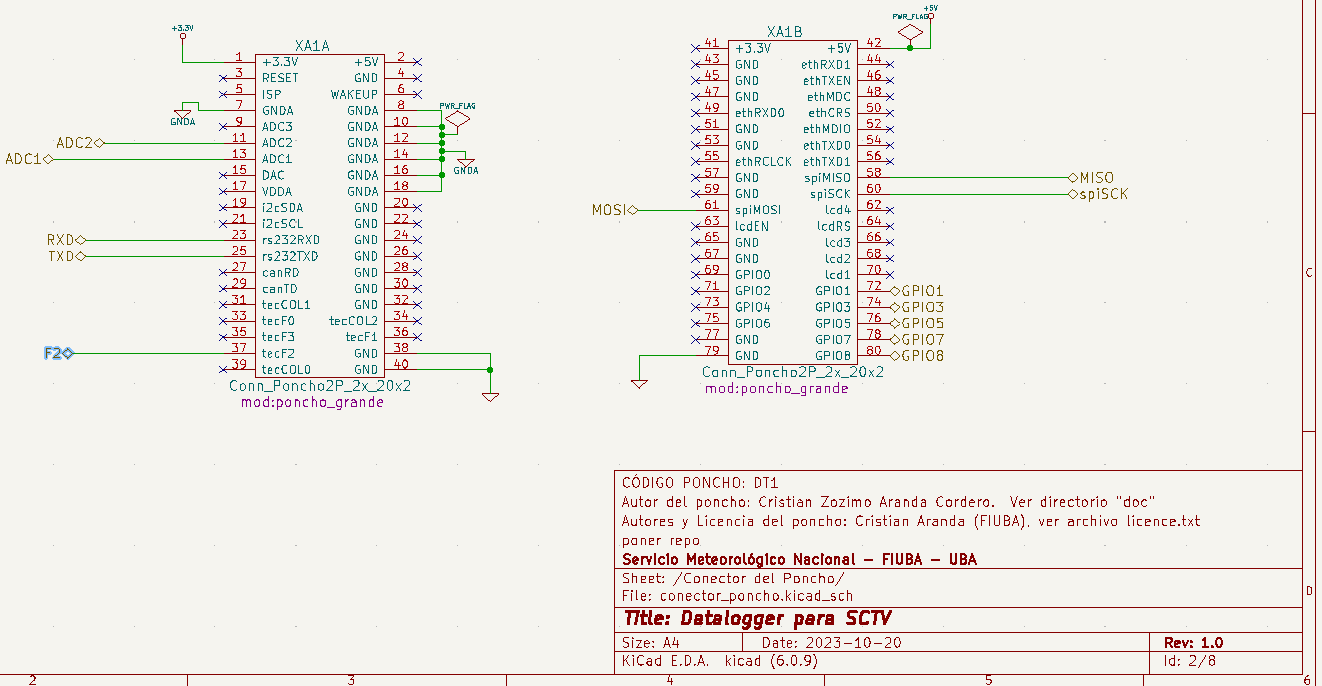
\includegraphics[width=0.95\linewidth]{Figuras/datalogger/Hardware/HojaTemplatePonchoCiaa.png}
    \caption{Template disponible para la realización de ponchos para la EDU-CIAA.}
    \label{fig:HojaTemplatePonchoCiaa}
\end{figure}


Por cada módulo, se agregó una hoja jerárquica que contiene el circuito esquemático como se indica en la Figura \ref{fig:esquematicoPonchoDatalogger}. En total, se dividió en seis hojas jerárquicas: una para el módulo RS485, otra para el módulo Ethernet W5100, otra para el circuito PWM, otra para la fuente de alimentación (power supply), otra para los LEDs y una más para el circuito que mide la tensión en el variador del túnel.

Además, se diseñaron los símbolos para los módulos W5100, RS485-TTL y el convertidor DC-DC usando el editor de símbolos de KiCad, ya que estos no vienen precargados en el software. También se diseñaron sus respectivos footprints con el editor de huellas, tomando las dimensiones y la distribución de pines de cada módulo para que se puedan agregar correctamente al PCB.

\begin{figure}[H]
    \centering
    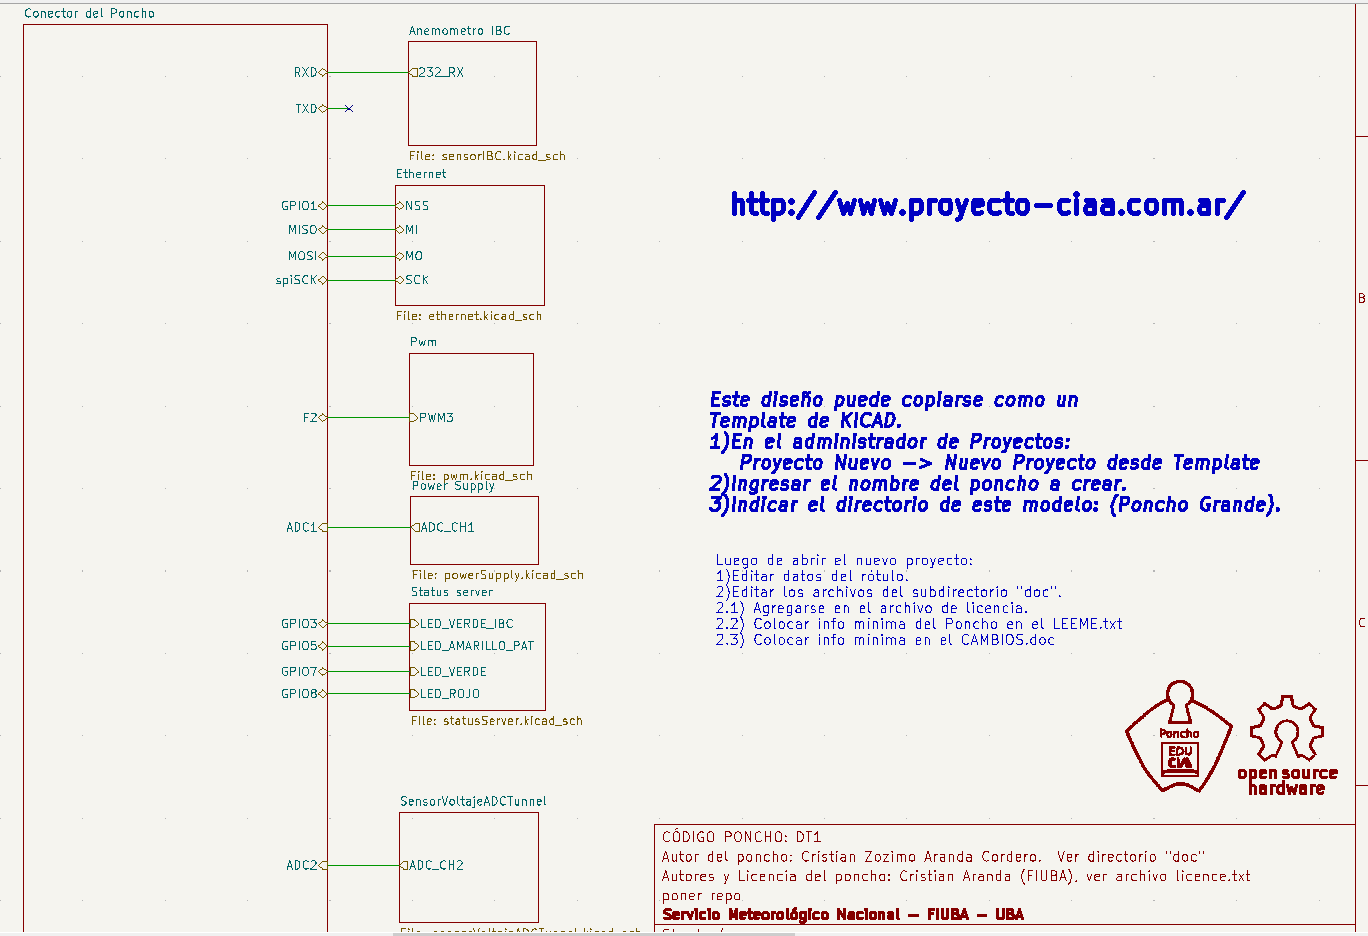
\includegraphics[width=0.95\linewidth]{Figuras/datalogger/Hardware/esquematicoPonchoDatalogger.png}
    \caption{Diseño del esquemático que integra los módulos desarrollados.}
    \label{fig:esquematicoPonchoDatalogger}
\end{figure}



% mostrar el diseño del poncho esquematico, PCB y la placa armada (fabricacion SMN o LCI)

En la Figura \ref{fig:pcbDesing} se muestra el diseño del PCB de doble capa, con la capa inferior (Bottom) en azul y la capa superior (Top) en rojo. Las dimensiones de los bordes recortados y la tira de 20 pines en la parte superior e inferior forman parte del template; el resto del circuito se diseñó en función de las necesidades de cada módulo.

Las pistas tienen un ancho de entre 30 y 40 mils. Se agregaron vías de \SI{2}{\milli\meter} de diámetro con un agujero de \SI{1}{\milli\meter} para conectar la capa superior con la capa inferior. Además, los pads tienen un tamaño de \SI{2}{\milli\meter}.


% Se armó el circuito con componentes SMD para la capa bottom y otro componetes thoguhole para la capa TOP, se hizo de esta forma poque 
\begin{figure}[H]
    \centering
    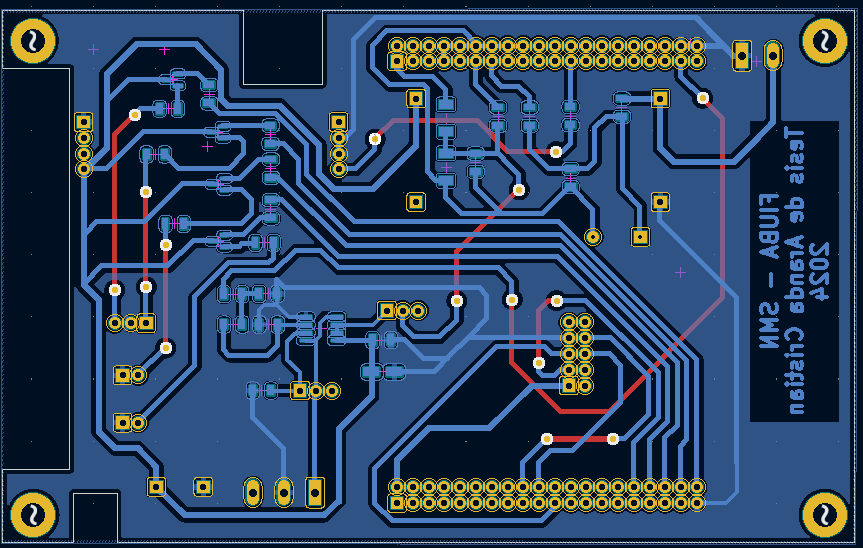
\includegraphics[width=0.95\linewidth]{Figuras/datalogger/Hardware/pcbDesing.png}
    \caption{Diseño PCB del Shield (poncho) que contiene todos los módulos descritos en las secciones anteriores.}
    \label{fig:pcbDesing}
\end{figure}

En la figura \ref{fig:pcb3dBottom} se muestra la vista 3D de capa Bottom donde se diseñó los circuitos PWM, el adquisidor de tensión de la fuente y el adquisidor de tensión del variador, utilizando componentes SMD. Se emplearon diodos, capacitores y resistores con tamaño de paquete 1206 y para los transistores NPN MMBT3904 y el operacional LM358 se cargaron sus footprints SMD de la biblioteca de KiCad.


\begin{figure}[H]
    \centering
    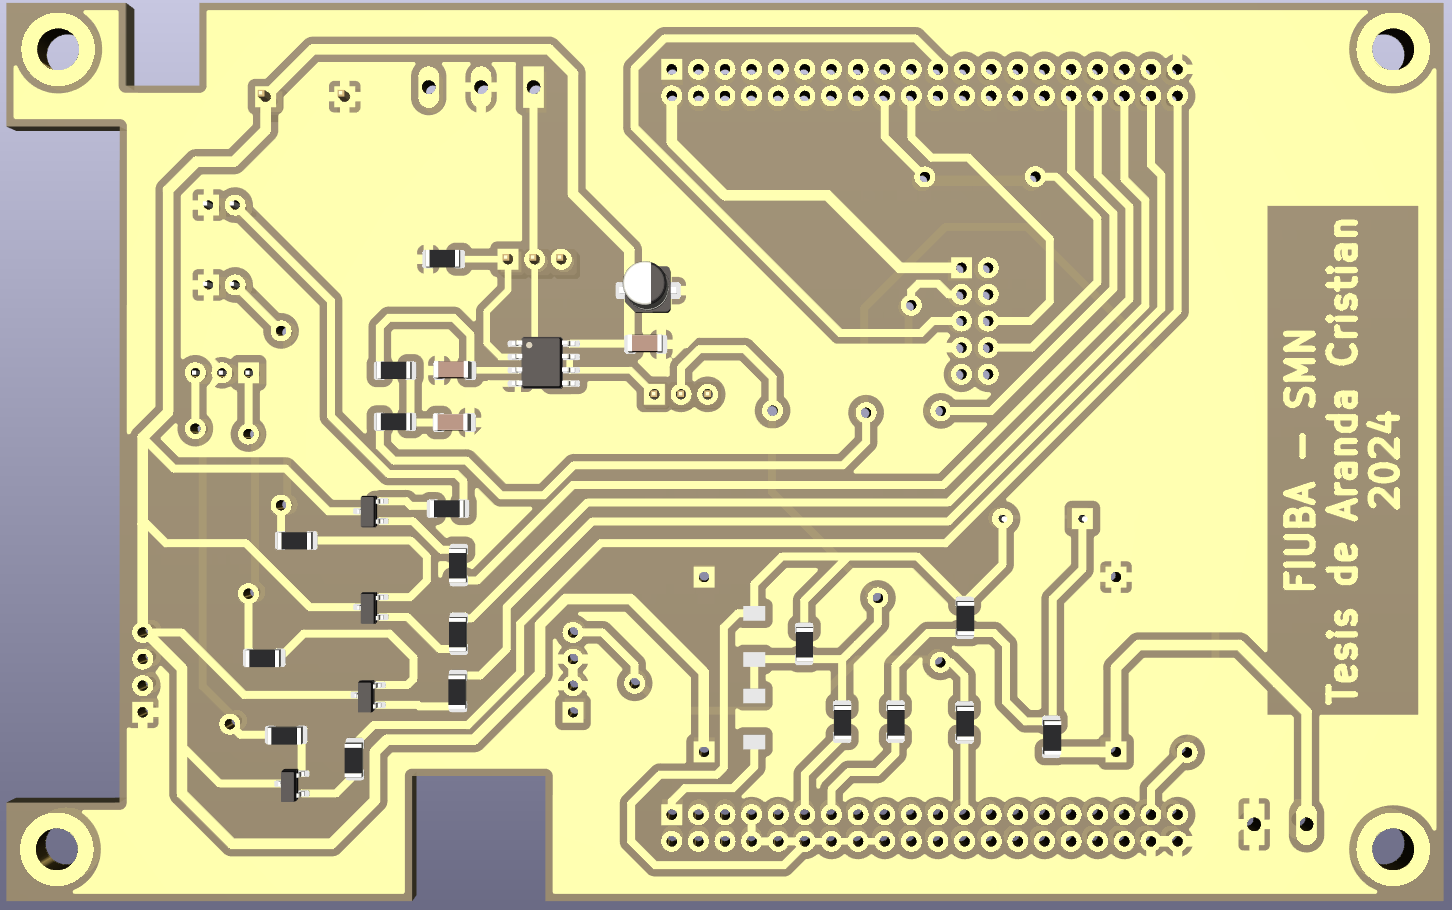
\includegraphics[width=0.95\linewidth]{Figuras/datalogger/Hardware/pcb3dBottom.png}
    \caption{Vista en 3D de la capa BOTTOM.}
    \label{fig:pcb3dBottom}
\end{figure}

Por otro lado, en la capa superior (TOP) se han añadido los tres LEDs con montaje THT y se han dispuesto dos tiras de pines 3x1 para la conexión física de los dos potenciómetros variables (presets). Además, debido a la falta de disponibilidad del diodo Zener SMD de \SI{3.3}{\volt} para proteger el ADC-CH1 de la placa EDU-CIAA, se adquirió el mismo componente pero con montaje THT. También se han incorporado los footprints de los módulos previamente diseñados del módulo Ethernet, módulo RS485-UART (que incluye su propia bornera para la conexión del anemómetro bajo calibración), y módulo DC-DC step-dowm. Además, se han agregado una bornera de 2x1 para alimentar el circuito con \SI{12}{\volt}, y otra bornera 3x1 para la conexión con el variador del túnel de viento.


\begin{figure}[H]
    \centering
    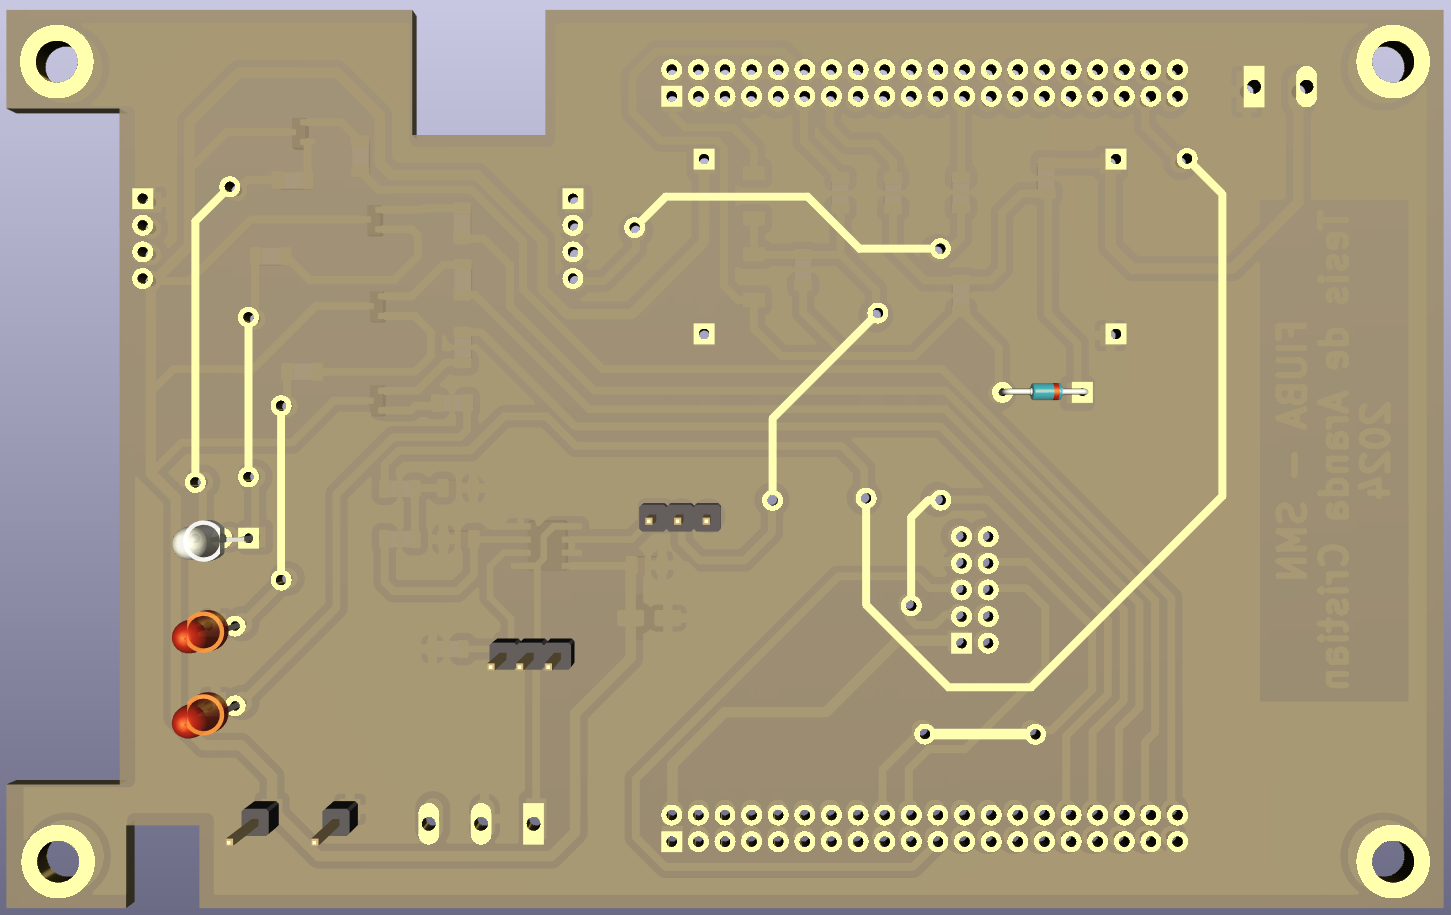
\includegraphics[width=0.95\linewidth]{Figuras/datalogger/Hardware/pcb3dTop.png}
    \caption{Vista en 3D de la capa TOP.}
    \label{fig:pcb3dTop}
\end{figure}

Para la construcción del \textit{shield}, se seleccionó una placa FAS simple por su disponibilidad en el Servicio Meteorológico Nacional (SMN). Debido a restricciones de tiempo, se optó por ensamblar la placa en el laboratorio del SMN, siguiendo estos pasos:

Inicialmente, se empleó una insoladora de tubos UV y papel fotosensible para transferir el diseño a la placa. Los negativos del diseño se imprimieron en papel transparente.

Después, se utilizó ácido perclórico para retirar el cobre sobrante. Finalizado este procedimiento, se cortó la placa a la medida deseada y se perforaron los \textit{pads} con una herramienta \textit{Dremel}. Se aplicó una capa de máscara antisoldante para facilitar la soldadura de los componentes y proteger la placa. Dado que la placa era de tipo FAS simple, se añadieron manualmente las pistas de la capa superior (Top) usando pequeños cables. El proceso concluyó con la soldadura de todos los módulos y componentes. Las Figuras \ref{fig:poncho1} y \ref{fig:poncho2} ilustran el resultado final del montaje.


\begin{figure}[H]
    \centering
    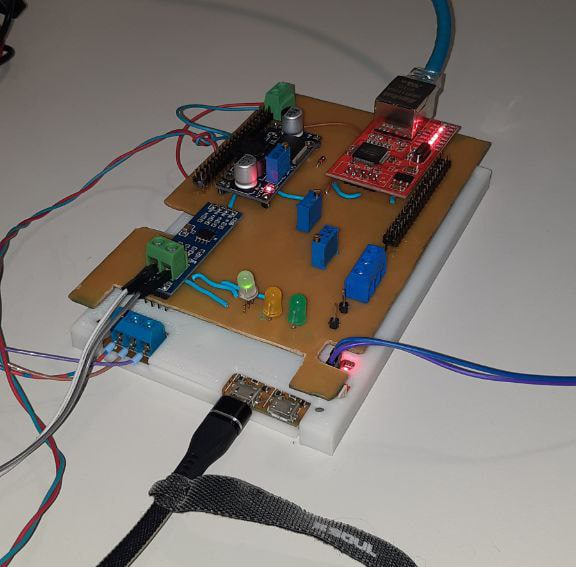
\includegraphics[width=0.6\linewidth]{Figuras/datalogger/Hardware/poncho1.jpg}
    \caption{Shield conectado a la placa EDU-CIAA}
    \label{fig:poncho1}
\end{figure}


\begin{figure}[H]
    \centering
    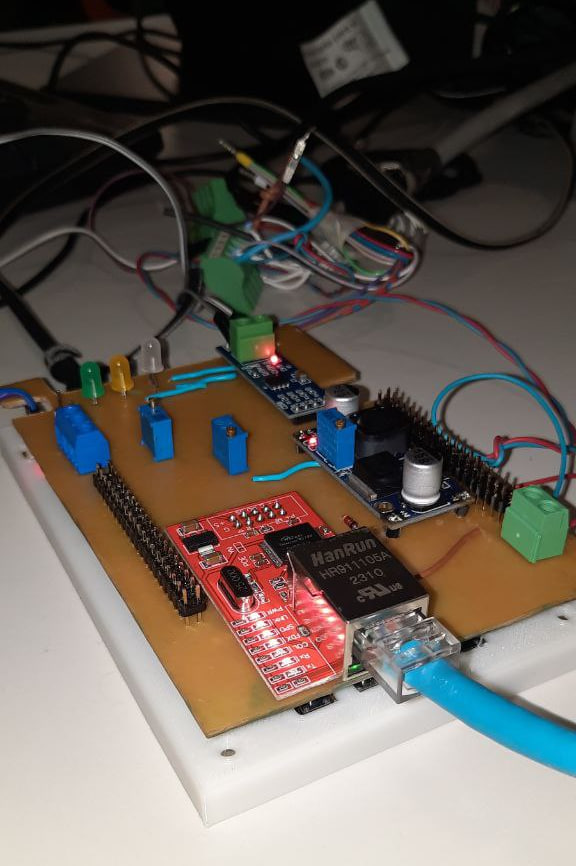
\includegraphics[width=0.5\linewidth]{Figuras/datalogger/Hardware/poncho2.jpg}
    \caption{Otra vista del Shield diseñado para esta aplicación.}
    \label{fig:poncho2}
\end{figure}

Como se indica en la Figura \ref{fig:poncho3}, se conectó el USB para programar y depurar la placa. Se conectó en la bornera azul de la EDU-CIAA el sensor patrón y en la bornera verde del módulo RS485 se conectó el anemómetro bajo calibración. En la parte superior de la figura está una  bornera azul, ahi se conectaron los tres cables que vienen del variador de velocidad del túnel. En el lado izquierdo, se conectó un cable UTP que está conectado a la red local del SMN, y en la bornera verde que está abajo a la izquierda,  se conectó la alimentación de \SI{12}{\volt}.

\begin{figure}[H]
    \centering
    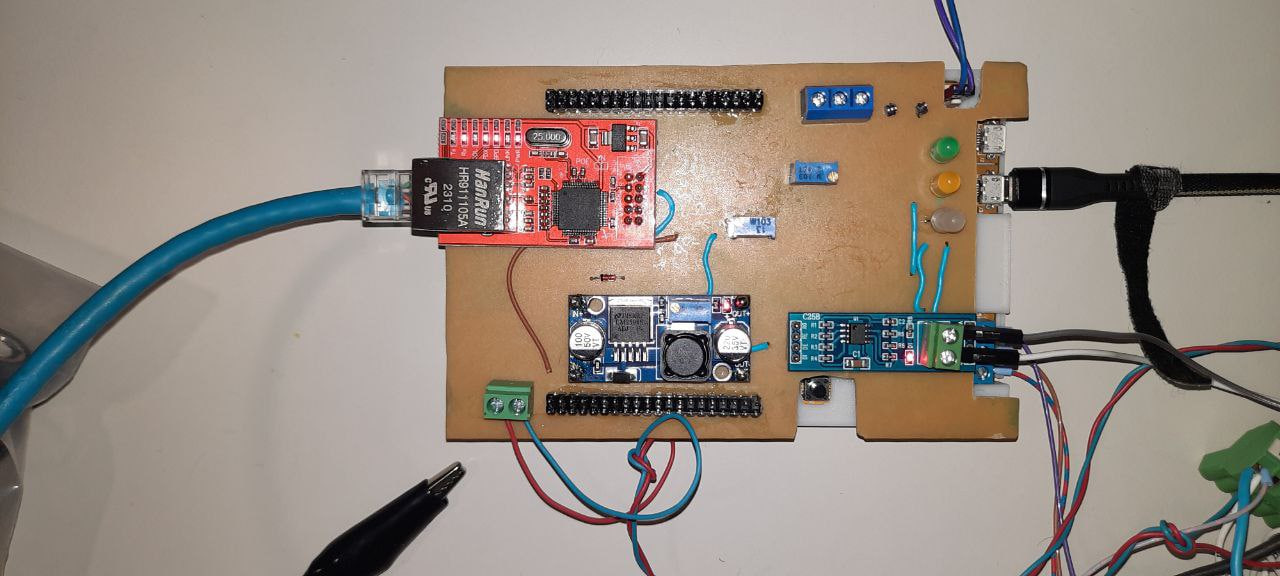
\includegraphics[width=1\linewidth]{Figuras/datalogger/Hardware/poncho3.jpg}
    \caption{Vista superior de la placa Shield conectada a la EDU-CIAA}
    \label{fig:poncho3}
\end{figure}


%%%%%%%%%%%%%%%%%%%%%%%%%%%%%%%%%%%%%%%%%%%%%%%%%%%%%%%%%%%%%%%%%%%%%%%%%%%%%%%%%%%%%%%%%%%%%%%%%%%%%%%
%-----------------------------------------------------------------------------------------------------
\section{Desarrollo del Firmware}\label{sec:desarrolloFirmware}

El proyecto CIAA brinda un framework para programar las placas de desarrollo. La última versión, el \texttt{firmware\_v3} \cite{ciaa2024}, es un proyecto basado en makefile para desarrollar firmware en C/C++. En particular se utilizó la biblioteca sAPI, que ofrece ejemplos para programar los periféricos del microcontrolador.

Además, el proyecto incluye un lanzador de aplicaciones Figura \ref{fig:ciaaLauncher}, que trae integrado el IDE GNU MCU Eclipse como entorno de programacion, OpenOCD para programcion y depuracion, drivers para conectar la EDU-CIAA a la PC, entre otras herramientas. 

\begin{figure}[H]
    \centering
    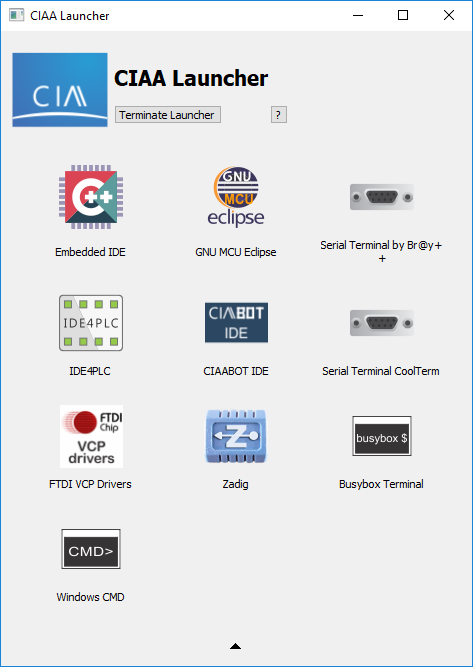
\includegraphics[width=0.35\linewidth]{Figuras/datalogger/Firmware/ciaaLauncher.png}
    \caption{Lanzador de aplicaciones integradas para el desarrollo de firmware para la EDU-CIAA.}
    \label{fig:ciaaLauncher}
\end{figure}

Se clonó el repositorio que contiene el \texttt{firmware\_v3} de GitHub en el IDE y se abrió un nuevo proyecto llamado \texttt{Datalogger}, como se indica en la Figura \ref{fig:projectDataloggerFolder}.

\begin{figure}[H]
    \centering
    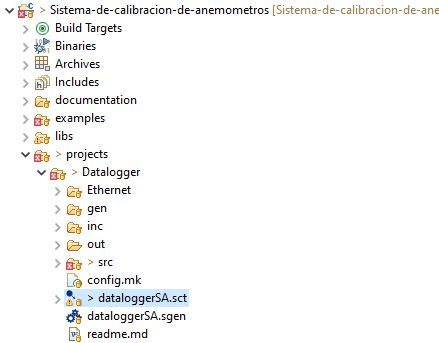
\includegraphics[width=0.40\linewidth]{Figuras/datalogger/Firmware/projectDataloggerFolder.jpg}
    \caption{Estructura de carpetas, del proyecto Datalogger}
    \label{fig:projectDataloggerFolder}
\end{figure}
En particular, la lógica del programa se implementó mediante el uso de maquinas de destado (\textit{statecharts}) de Harel, empleando el software Itemis Yakindu. Los \textit{statecharts} de Harel amplían los diagramas de estados tradicionales incorporando conceptos de modularidad, jerarquía y estructura organizacional. Estos diagramas se caracterizan por el uso de estados compuestos y subdiagramas que preservan la claridad y la organización, y facilitan la ejecución concurrente de múltiples submáquinas de estado a través de regiones ortogonales. Además, los eventos habilitan la comunicación por difusión, mientras que las transiciones condicionales, los estados históricos, la lógica temporal y las acciones de entrada/salida potencian la funcionalidad de los \textit{statecharts}, optimizando la modelización de sistemas complejos de manera eficiente. La Tabla~\ref{tab:compStateCharts} presenta un análisis comparativo entre las máquinas de estado simples, como las de Mealy y Moore, y las máquinas de estado más avanzadas de UML y Harel.


\begin{table}[H]
\begin{tblr}{
  colspec = {Q[l,8cm] Q[c,1.5cm] Q[c,1.5cm] Q[c,1.5cm] Q[c,1.5cm]},
  rows = {m},
  % row{1} = {font=\bfseries},    
  % cells = {c},
  row{1} = {Sail,font=\bfseries},
  hlines,
  vlines,
}
Descripción & Mealy     & Moore    & Harel    & UML \\
Estados y transiciones & \checkmark & \checkmark    & \checkmark    & \checkmark \\
Las transiciones producen salida & \checkmark   & \crossmark    & \checkmark    & \checkmark\\
Los estados producen salida & \crossmark    & \checkmark    & \checkmark    & \checkmark \\
Profundidad (jerarquías, estados compuestos) & \crossmark   & \crossmark & \checkmark   & \checkmark \\
Ortogonalidad (submáquinas de estado paralelas) & \crossmark    & \crossmark    & \checkmark    & \checkmark\\
Comunicación por difusión (eventos) & \crossmark    & \crossmark    & \checkmark    & \checkmark\\
Historial, acciones, retrasos, tiempos de espera, condiciones & \crossmark    & \crossmark    & \checkmark    & \checkmark\\
\end{tblr}
\caption{Diferencias entre los tipos de máquinas de estados.}
\label{tab:compStateCharts}
\end{table}
Se crearon doce regiones que trabajan de forma concurrente (de forma ortogonal), como se muestra en la Figura \ref{fig:ordenRegiones}, y se comunican entre sí mediante eventos internos. A cada región se le asigna una prioridad en función de su posición; las que están más arriba tienen mayor prioridad de ejecución respecto a las de más abajo.

\begin{figure}[H]
    \centering
    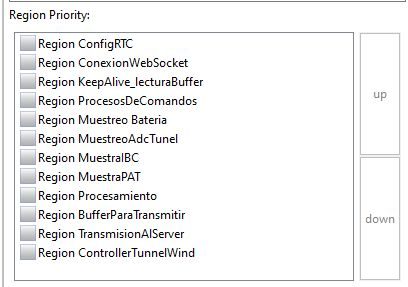
\includegraphics[width=0.5\linewidth]{Figuras/datalogger/Firmware/ordenRegiones.jpg}
    \caption{Lista de regiones con su respectiva prioridad.}
    \label{fig:ordenRegiones}
\end{figure}

Se utilizó una licencia gratuita de Yakindu, integrándola con el IDE de Eclipse para editar y generar el código a partir de los \textit{statecharts}. En particular, se configuró el proyecto en Yakindu C/C++ para poder agregar código en C a las máquinas de estado, incluyendo la importación de archivos \texttt{.h}, declaración de variables, punteros globales y constantes, como se ejemplifica en el Código \ref{cdg:configuracionStateChart}.



\begin{lstlisting}[style=yakindustyle, caption={Configuración principal del modelo statechart dataloggerSA.}, label=cdg:configuracionStateChart]
import:"inc/common.h"
import:"inc/da_acquisition.h"
import:"inc/da_processing.h"
import:"inc/da_transmision.h"
import:"inc/da_rtc.h"
import:"inc/da_configDatalogger.h"
import:"inc/controlTunnel.h"
/*Datalogger para Sistema anemometrico con EDU-CIAA-NXP */
interface:
//Variables
var startMesuare:uint8_t = FALSE
//Puntero
var ptrStartMesuare:ptrUnt8_t
var viTeclaOprim: uint16_t
//Constantes
const TRUE: uint8_t =1
const FALSE: uint8_t =0
const Tec1: uint16_t = 1<<0
const Tec2: uint16_t = 1<<1
\end{lstlisting}
 
 También se agregaron eventos internos que permiten transicionar del estado de una región a otro estado de otra región (\textit{raiseEvent} en inglés), como se muestra en el Código \ref{cdg:eventosInternos}.
\begin{lstlisting}[style=yakindustyle, caption={Declaración de eventos internos que permiten transicionar entre regiones del statechart.}, label=cdg:eventosInternos]
internal:
//En forma interna tengo seniales para vincular las maquinas de estado
event siDatosListosParaBdtos
event siDatoProcesado
event siMuestrasNuevas
event siStartMeasure
event siKeepAlive
event siProccesMsjServer
\end{lstlisting}

% En cada subseccion agregar su region de yakindu

%%%%%%%%%%%%%%%%%%%%%%%%%%%%%%%%%%%%%%%%%%%%%%%%%%%%%%%%%%%%%%%%%%%%%%%%%%%%%%%%%%%%%%%%%%%%%%%%%%%%%%%
\subsection{Configuración y conexión con los servidores}\label{sec:confServers}
Como se detalló en la sección \ref{sec:moduloEthernet}, se utilizó el módulo W5100 para transferir datos desde el datalogger hacia los servidores y recibir datos de los mismos. El módulo cuenta con cuatro socket independientes y permite configurar un sistema embebido como servidor o cliente, como se muestra en la Figura \ref{fig:socketModoDeTrabajoW5100}.

\begin{figure}[H]
    \centering
    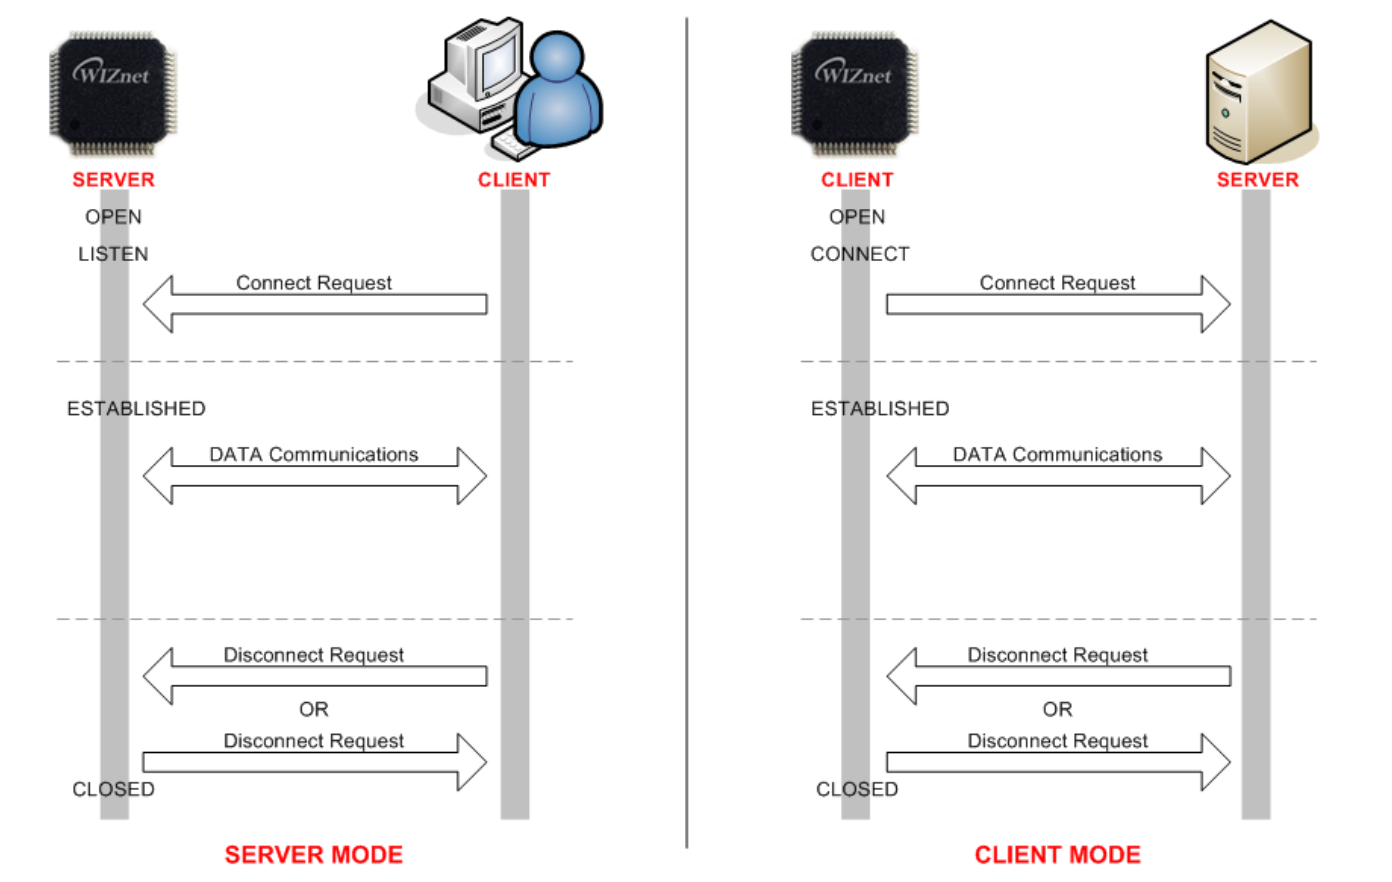
\includegraphics[width=0.9\linewidth]{Figuras/datalogger/Firmware/socketModoDeTrabajoW5100.png}
    \caption{Modos de configuración para el módulo W5100.}
    \label{fig:socketModoDeTrabajoW5100}
\end{figure}

El datalogger se comunica con los servidores en modo cliente (apertura activa), enviando una solicitud de conexión a un servidor, estableciendo la comunicación e intercambiando datos. Luego, realiza una solicitud de desconexión y se cierra el enlace. Utiliza, en la capa de transporte, el protocolo TCP y, en la capa de red, el protocolo IP. En la capa de aplicación, se utilizó el protocolo WebSocket para intercambio de datos y el protocolo NTP para configurar el RTC del datalogger. Dado que estos protocolos no están incluidos en la biblioteca del chip W5100, se implementó la conexión, el intercambio de datos y la desconexión de los servidores mediante sockets, como se indica en el diagrama de flujo de la figura \ref{fig:socketDiagramClientW5100}.

Un socket es una interfaz que permite la comunicación entre dispositivos a través de redes. En términos simples, un socket es un punto final para enviar y recibir datos en una red, y está compuesto por una dirección IP y un número de puerto.
\begin{figure}[H]
    \centering
    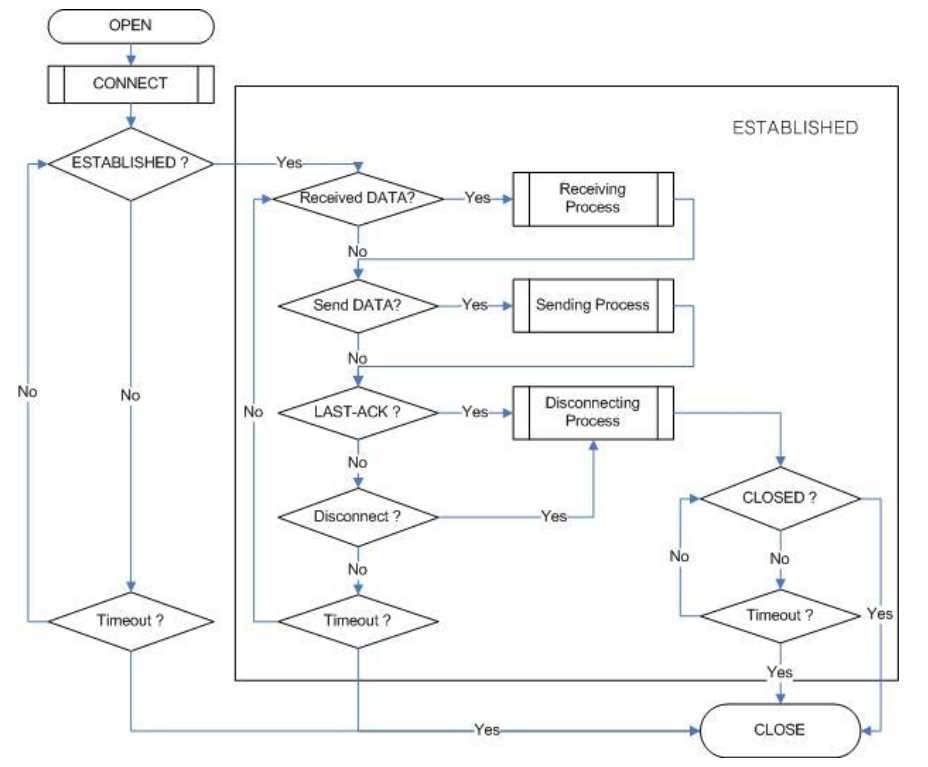
\includegraphics[width=0.9\linewidth]{Figuras/datalogger/Firmware/socketDiagramClientW5100.png}
    \caption{Diagrama de flujo para establer una comunicación, en modo cliente, con un servidor utilizando sockets.}
    \label{fig:socketDiagramClientW5100}
\end{figure}

\subsubsection{Servidor NTP}\label{sec:serverNTP}
% poner diagrama de Config RTC, para que esta
Para la configuración del RTC del datalogger, se estableció una conexión con los servidores NTP del Instituto Nacional de Estándares y Tecnología (\textit{NIST}). Se seleccionó una de las múltiples IPs disponibles, específicamente la dirección 128.138.141.172 a través del puerto 13. Esta conexión retorna una cadena de caracteres, \texttt{59992 23-02-17 17:47:01 00 0 0 831.5 UTC(NIST)*}, que se procesó e integró en la estructura del RTC del datalogger. Para gestionar y validar esta comunicación con el servidor NTP, se configuró una región específica dentro del sistema. Las variables declaradas en el Código \ref{cdg:serRTC} se utilizan para validar cada transición dentro de la máquina de estados ilustrada en la Figura \ref{fig:ntpServer}.


\begin{lstlisting}[style=yakindustyle, caption={Declaración de variables booleanas para validar la conexion con el servidor NTP.}, label=cdg:serRTC]
// Variables para la conexion al servidor NTP
var ConfigNtpSocket: uint8_t=FALSE
var setRtc: uint8_t = FALSE
var ConfigNTP:uint8_t = FALSE
\end{lstlisting}

La máquina comienza en el estado \textbf{INIT} y luego de un período de \texttt{DelatInit} segundos, pasa al estado \textbf{CONFIG\_SOCKET}. En este estado, se llama a la función \texttt{opConfigNtpSocketViaTCP()}, que se encarga de configurar los parámetros de red del cliente: gateway, dirección MAC, máscara de subred e IP. 

Luego, estos parámetros se asignan a uno de los cuatro sockets del módulo W5100, y se configura el protocolo de transporte (TCP en este caso), el puerto, y se abre la conexión para establecer una comunicación con el servidor. Esta función devuelve \texttt{True} si la apertura y configuración son correctas, almacenando este resultado en la variable \texttt{ConfigNtpSocket}. Si la configuración es exitosa, la máquina de estados transiciona al estado \textbf{CONFIG\_NTP}.

En el estado \textbf{CONFIG\_NTP}, se invoca la función \texttt{opConfigNtpViaTCP()}, encargada de configurar la conexión con el servidor NTP. Esta función establece la dirección IP y el puerto del servidor y realiza un intento de conexión. Si la conexión es exitosa, la función retorna \texttt{True} y el resultado se almacena en la variable \texttt{ConfigNTP}. Una vez configurado, el servidor responde con la hora y fecha actual en formato UTC, que se guarda en una variable interna. Posteriormente, la máquina de estados avanza al estado \textbf{SET\_RTC\_VIA\_SOCKET}, donde se procesa la información recibida y se actualiza el RTC del datalogger. Finalmente, se cierra la conexión con el servidor NTP pasando al estado \textbf{IDLE}, cuando se realiza esta última transición se eleva un evento a través de la señal \texttt{siStartMeasure}, la cual será un disparador para iniciar otra máquina de estado en otra región. En caso de fallo en cualquiera de los estados previos, se transiciona al estado \textbf{SET\_RTC\_DEFAULT}, donde se establece una hora predeterminada.

\begin{figure}[H]
    \centering
    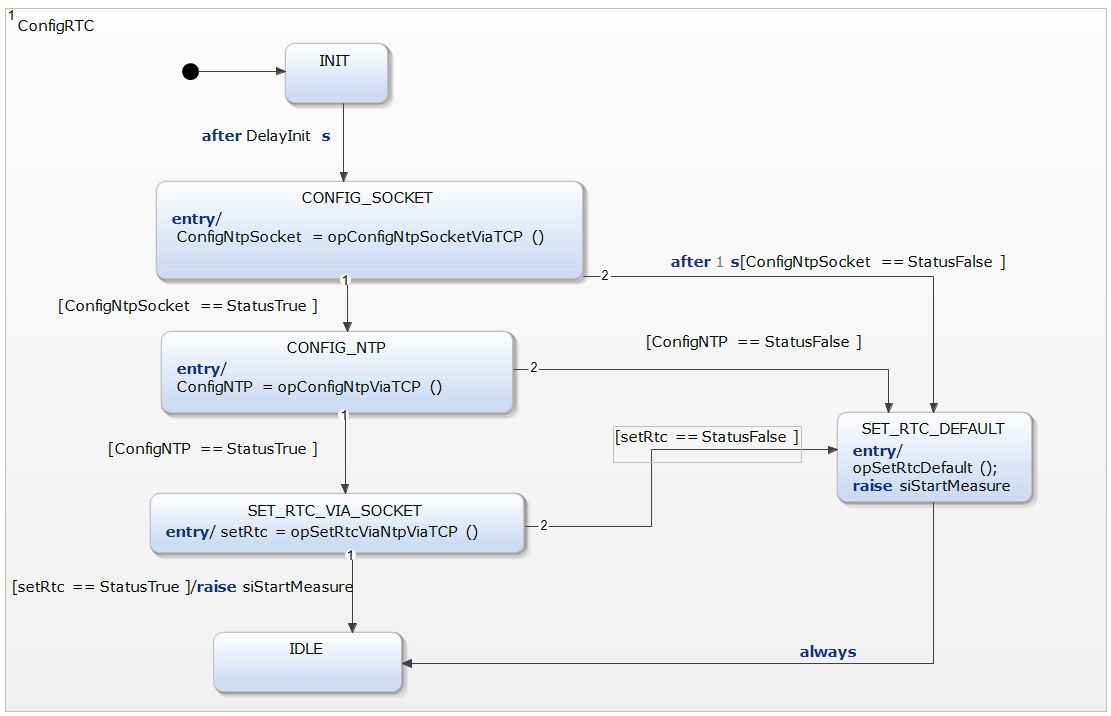
\includegraphics[width=0.9\linewidth]{Figuras/datalogger/Firmware/ntpServer.jpg}
    \caption{Máquina de estados para configurar el RTC del datalogger a través de un servidor NTP.}
    \label{fig:ntpServer}
\end{figure}

\subsubsection{Servidor WebSocket}\label{sec:serverWebSocket}
 
El protocolo WebSocket es una tecnología de comunicación que permite interacciones bidireccionales (\textit{full-duplex}) entre un cliente y un servidor a través de un solo canal de conexión TCP. Es especialmente útil para aplicaciones web que requieren comunicación en tiempo real, como juegos en línea, chat en vivo y servicios de trading. Para establecer una conexión WebSocket, el cliente envía una solicitud de  \textit{handshake} (aprenton de manos) al servidor. Esta solicitud sigue el protocolo HTTP con un \textit{upgrade} para solicitar el cambio de protocolo a WebSocket. Aquí se muestra un ejemplo de cómo se ve una solicitud de \textit{handshake} de WebSocket:

\begin{verbatim}
GET /mychat HTTP/1.1
Host: 10.10.13.153
Upgrade: websocket
Connection: Upgrade
Sec-WebSocket-Key: x3JJHMbDL1EzLkh9GBhXDw==
Sec-WebSocket-Protocol: chat, superchat
Sec-WebSocket-Version: 13
Origin: http://example.com
\end{verbatim}

El servidor, al recibir esta solicitud, responde con una respuesta de \textit{handshake} si acepta la conexión:

\begin{verbatim}
HTTP/1.1 101 Switching Protocols
Upgrade: websocket
Connection: Upgrade
Sec-WebSocket-Accept: HSmrc0sMlYUkAGmm5OPpG2HaGWk=
Sec-WebSocket-Protocol: chat
\end{verbatim}

La clave \texttt{Sec-WebSocket-Accept} es generada por el servidor a partir de la clave \texttt{Sec-WebSocket-Key} enviada por el cliente, lo que confirma que el servidor entiende y acepta la solicitud de WebSocket. Una vez establecido el \textit{handshake}, el cliente y el servidor pueden enviar datos en forma de \textit{frames} de WebSocket, que pueden ser datos de texto o binarios.

A Continuación se pasa a explicar como se implementó la comunicación. Para ello se declaran las variables de estado que se muestran en el Código \ref{cdg:setWebSocket} y permiten la transición de estados de la región \texttt{ConexionWebSocket} que se muestra en la figura \ref{fig:connectWebSocket}

\begin{lstlisting}[style=yakindustyle, caption={Declaración de variables booleanas para validar la conexion con el servidor WebSocket.}, label=cdg:setWebSocket]
// Variables para la conexion al servidor WebSocket
ar socketConnect: uint8_t = FALSE
var isConnectWebServer: uint8_t=FALSE
var buffertempLleno: uint8_t = TRUE
var txKeep:uint8_t=FALSE
\end{lstlisting}

La máquina de estados inicia en el estado \textbf{IDLE}. La transición al estado \textbf{CONFIG\_SOCKET} se desencadena por el evento de la señal \texttt{siStartMeasure}, generado tras la correcta configuración del tiempo por la máquina de estados del servidor NTP. Esto asegura que no se inicie la medición hasta que la hora esté precisamente sincronizada. En el estado \textbf{CONFIG\_SOCKET}, se invoca la función \texttt{opConfigSocket()}, responsable de configurar los parámetros de red del módulo W5100, incluyendo el gateway, la máscara de subred, la dirección MAC y una dirección IP. También se establece el protocolo TCP, asignando un número de puerto al cliente. Tras abrir el socket, la máquina de estados avanza al estado \textbf{INI\_WEB\_SOCKET} sin requerir validación adicional.

En el estado \textbf{INI\_WEB\_SOCKET}, se ejecuta la función \texttt{opInitWebSocket()}, que prepara los datos necesarios para la conexión con el servidor WebSocket, como la dirección IP del servidor y el puerto. Esta configuración permite actualizar la variable \texttt{socketConnect} a \texttt{True}, habilitando el avance al estado \textbf{CONNECT\_WEBSOCKET}. Aquí, la función \texttt{opConnectToWebSocket()} gestiona el envío de la solicitud de \textit{handshake} al servidor y procesa su respuesta. Si la conexión es exitosa, la variable \texttt{isConnectWebServer} se establece en \texttt{True}, indicando que la conexión está lista para el intercambio de datos en modo full-duplex.

Si se presenta un fallo en cualquiera de los estados previos, la máquina de estados regresa al estado \textbf{CONFIG\_SOCKET} para intentar una nueva conexión con el servidor.

\begin{figure}[H]
    \centering
    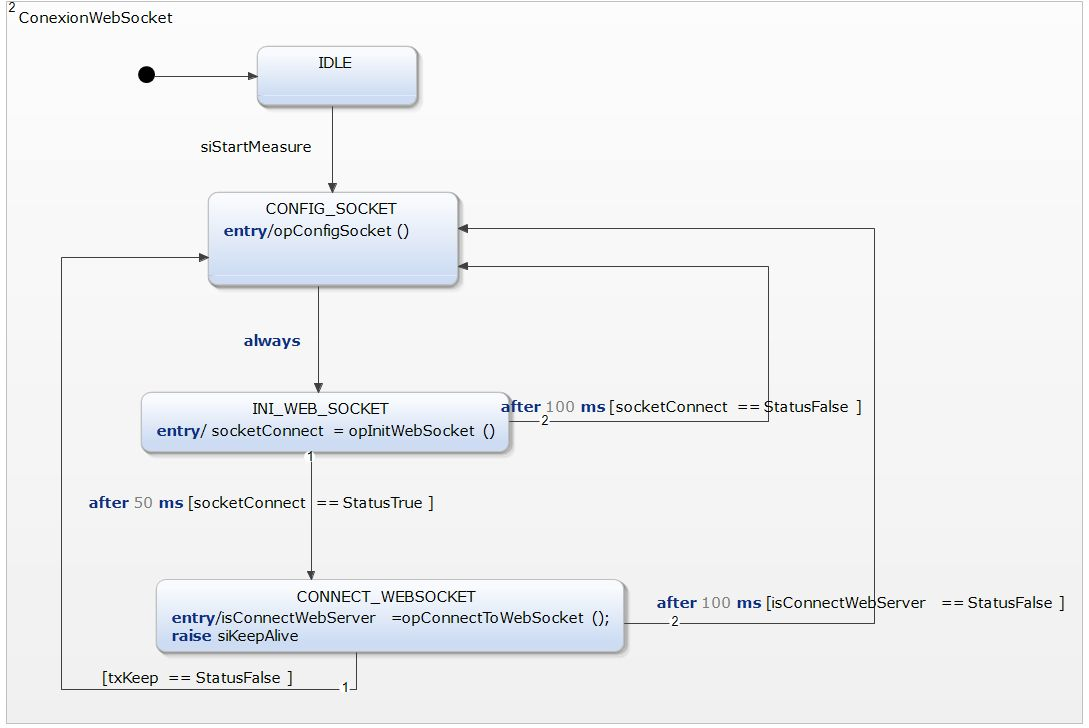
\includegraphics[width=0.9\linewidth]{Figuras/datalogger/Firmware/connectWebSocket.jpg}
    \caption{Máquina de estados para establecer una conexión bidireccional con un servidor WebSocket.}
    \label{fig:connectWebSocket}
\end{figure}
% Luego hablar del keep alive 

Para prevenir la desconexión automática del protocolo WebSocket en ausencia de intercambio de datos, se implementó una región denominada \texttt{KeepAlive\_lecturaBuffer}. Esta región tiene un doble propósito: primero, mantener activa la comunicación con el servidor incluso cuando no hay tráfico de datos; y segundo, realizar una consulta periódica (\textit{polling}) con un retardo no bloqueante para verificar si se ha recibido algún mensaje del servidor.

El estado final de la región \texttt{ConexionWebSocket} de la Figura \ref{fig:connectWebSocket}, al completar su secuencia de operaciones, genera un evento con la señal \texttt{siKeepAlive}. Esta señal, en conjunción con la condición de que \texttt{isConnectWebServer} esté establecida en \texttt{True}, facilita la transición desde el estado \textbf{IDLE} hacia el estado \textbf{TX\_MESSAGE}. En este último estado, se pueden transmitir mensajes al servidor, manteniendo así la conexión WebSocket activa y funcional.

% En este estado se invoca a la función \texttt{KeepAlive(ptrSizeBuff)} que se encarga de enviar un mensaje vacío al servidor para mantener la comunicación y revisar si hay algún mensaje del servidor guardándolo en un buffer. En caso de 


\begin{figure}[H]
    \centering
    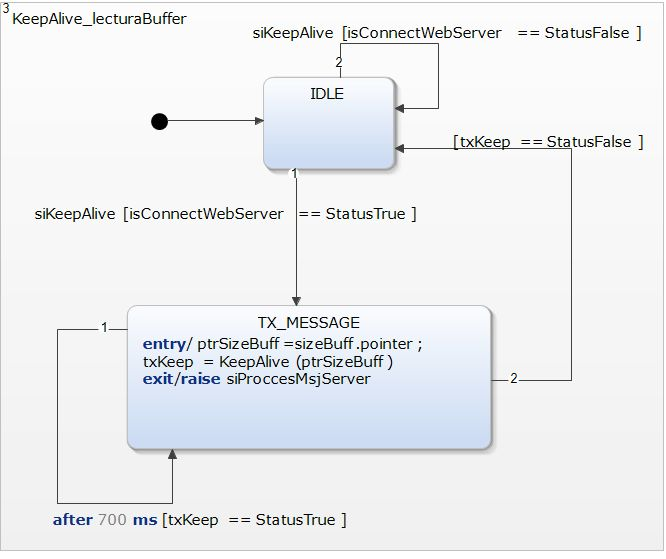
\includegraphics[width=0.6\linewidth]{Figuras/datalogger/Firmware/keepAlive.jpg}
    \caption{Máquina de estados para mantener la conexión con el servidor y elevar un raise en caso de que se reciba información del servidor.}
    \label{fig:keepAlive}
\end{figure}

% La recepcion de comandos para configurar
Puesto que se puede recibir datos del servidor, se declaran las siguientes variables del Código \ref{cdg:SetCommanBuffer}

\begin{lstlisting}[style=yakindustyle, caption={Declaración de variables para validar y procesar la recepción de datos del servidor.}, label=cdg:SetCommanBuffer]
//Procesamiento de comandos
//Size de comandos
var sizeBuff: uint16_t =0
var ptrSizeBuff: ptrUnt16_t
//Estructura de configuracion a traves de comandos
var configCommand:config_t
var ptrConfigCommand:ptrConfig_t=configCommand.pointer
\end{lstlisting}

En el estado \textbf{TX\_MESSAGE}, independientemente de si se han recibido datos del servidor, se genera un evento hacia la región \texttt{ProcesoDeComandos}. Este evento facilita la transición del estado \textbf{IDLE} al estado \textbf{PROCESS\_COMMAND}, condicionada a que la longitud del mensaje recibido del servidor sea mayor a cero. Si se cumple esta condición, en el estado \textbf{PROCESS\_COMMAND} se invoca la función \texttt{opProcessMessageFromServer(ptrSizeBuff, ptrConfigCommand)}, que se encarga de procesar los mensajes provenientes del servidor. Estos mensajes pueden incluir comandos de configuración para el datalogger o valores de referencia para el control del túnel, los cuales serán detallados en la sección \ref{sec:sistemaDeControlPid}.

\begin{figure}[H]
    \centering
    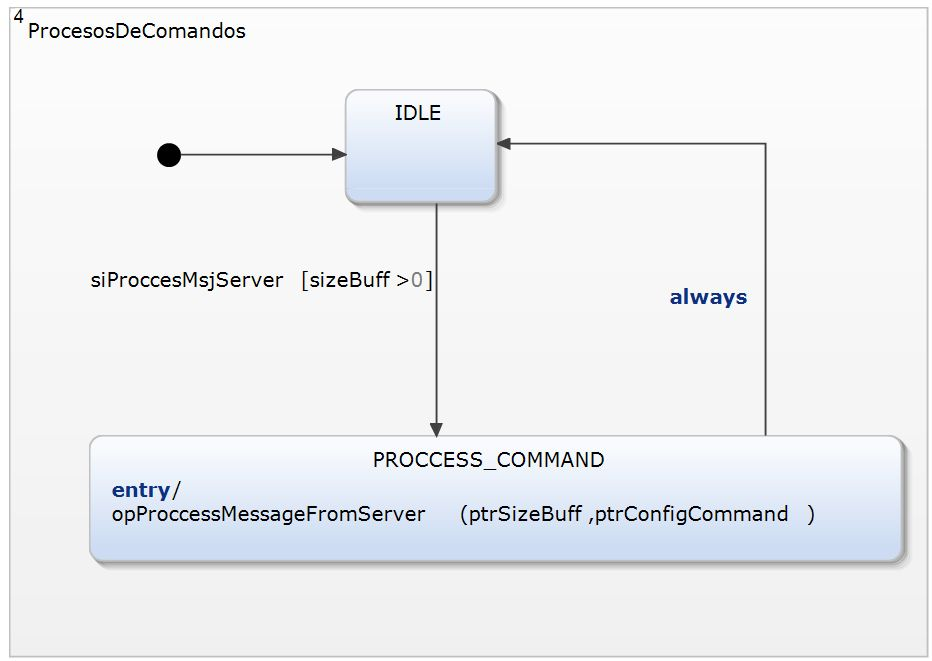
\includegraphics[width=0.6\linewidth]{Figuras/datalogger/Firmware/processComand.jpg}
    \caption{Máquina de estados para procesar los mensajes recibidos del servidor WebSocket.}
    \label{fig:processComand}
\end{figure}

Para gestionar eficientemente los comandos destinados a configurar diversas partes del datalogger con la información proporcionada por el software, se establece un diccionario de punteros a función. Este diccionario, ilustrado en el código~\ref{cdg:diccCommand}, permite ejecutar una función específica en respuesta a cada comando o petición contenida en el mensaje recibido.

\begin{lstlisting}[style=cstyle, caption={Funciones que permiten configurar o modificar el comportamiento del dataloger.}, label=cdg:diccCommand]
char *diccCommands[]={
				"start",
				"stop",
				"setIBC",
				"setPAT",
				"setTimes",
				"refWindVel",
				"NAN"};
bool_t (*diccProcesos[])(config_t * commandConfig)={
							start,
							stop,
							setIBC,
							setPAT,
							setTimes,
							refWindVel};

\end{lstlisting}


%%%%%%%%%%%%%%%%%%%%%%%%%%%%%%%%%%%%%%%%%%%%%%%%%%%%%%%%%%%%%%%%%%%%%%%%%%%%%%%%%%%%%%%%%%%%%%%%%%%%%%%
\subsection{Muestreo, adquisición y procesamiento}\label{sec:muestreo_adquisicion_procesamiento}

Para almacenar las muestras de los sensores de viento, patrón y bajo calibración, así como los niveles de tensión de la fuente y la tensión que ingresa al variador de velocidad, se han declarado las variables, punteros y constantes mostrados en el Código \ref{cdg:var_const_Adquisition}. Cada variable está asociada a un puntero, ya que cada función de cada estado o transición requiere recibir un puntero específico a una variable para poder modificar su valor.

\begin{lstlisting}[style=yakindustyle, caption={Variables para almacenar en cada iteración una muestra de su magnitud correspondiente.}, label=cdg:var_const_Adquisition]
//Variable interna para guardar las muestras de voltaje DC
var viVoltajeMuestra: real32_t
//Puntero Correspodiente
var ptrVoltajeMuestra: ptrReal32_t
//MuestraDelAdcDelTunnel
//Variable interna para guardar las muestras de voltaje DC
var viTunelTensionMuestra: real32_t
//Puntero Correspodiente
var ptrTunelTensionMuestra: ptrReal32_t
// IBC
var ptrAnemoIBC:ptrAmenometerSerialParam_t =configCommand.AnemoIBC.pointer
//PAT
var ptrAnemoPat:ptrAmenometerSerialParam_t=configCommand.AnemoPAT.pointer

\end{lstlisting}

% \begin{figure}[H]
%     \centering
%     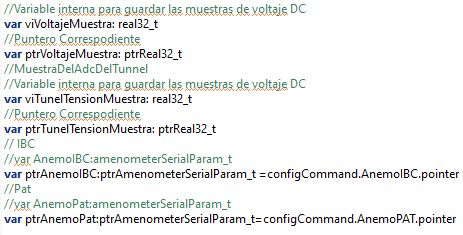
\includegraphics[width=0.6\linewidth]{Figuras/datalogger/Firmware/var_const_Adquisition.jpg}
%     \caption{Variables para almacenar en cada iteración una muestra de su magnitud correspondiente.}
%     \label{fig:var_const_Adquisition}
% \end{figure}

Para configurar cada anemómetro, se ha declarado una estructura como se muestra en el fragmento de código \ref{cdg:estructuraAnemo}. Esta estructura se inicializa con datos ingresados por el operador a través de la aplicación web descrita en el capítulo \ref{cap:aplicacionweb}. Cada estructura requiere configurar el número de \texttt{Uart}, el \texttt{LED} de recepción y el \texttt{BaudRate}, valores que deben coincidir con las especificaciones de cada anemómetro. Además, se dispone de un buffer de 100 caracteres para almacenar los strings de datos recibidos, con un puntero asociado para modificar su contenido. También se incluyen dos arreglos de números reales para almacenar los datos numéricos convertidos a \texttt{real32\_t} a partir de los strings de cada sensor, cada uno con su respectivo puntero para su modificación. Por último, se introduce el tipo de dato del sensor, \texttt{sensor\_t}, que enumera los sensores utilizados.



% Ejemplo codigo en c agregado desde un archivo
% \lstinputlisting[style=cstyle, caption={Ejemplo de código en C.}, label=lst:estructuraAnemo]{Codigos/estructuraAnemo.c}
% Ejemplo de código C copiando el codigo 
\begin{lstlisting}[style=cstyle, caption={Estructura de datos para anemómetro.}, label=cdg:estructuraAnemo]
typedef struct{
	uint16_t Uart;
	uint16_t LED;
	uint32_t BaudRate;
	char Buffer[100];
	char * ptrUartBuffer;
	real32_t DataAnemometer[7];
	real32_t * ptrDataAnemometer;
	sensor_t Sensor;
}amenometerSerialParam_t;
\end{lstlisting}
 
En las Figuras \ref{fig:MuestraIBC} y \ref{fig:MuestraPAT} se muestran las regiones que contienen las máquinas de estado \textbf{MuestraIBC} y \textbf{MuestraPAT}, respectivamente, para adquirir los datos de viento. La máquina de estado, por ejemplo, del IBC comienza en el estado \textbf{IDLE}. Cuando el comando \texttt{startMeasure} es \texttt{True}, se transiciona al estado \textbf{SENSOR\_IBC}, donde se invoca la función \texttt{opBufferRS485\_On(prtAnemo)}. Esta función recibe un puntero con todos los datos de configuración del anemómetro y los carga en su respectiva UART. Además, inicializa un callback y habilita la interrupción correspondiente de la UART. De esta manera, cada vez que los sensores envían datos, se activa una función que se encarga de procesar y separar los datos recibidos. Cuando \texttt{startMeasure} se configura como \texttt{false}, la máquina de estado transiciona al estado \textbf{OFF\_SENSOR\_IBC}, donde se desactiva la interrupción y el microcontrolador deja de tomar muestras de los anemómetros.

\begin{figure}[H]
    \centering
    \begin{subfigure}[b]{0.45\textwidth}
        \centering
        \includegraphics[width=1.2\linewidth]{Figuras/datalogger/Firmware/MuestraIBC.jpg}
        \caption{Máquina de estados para tomar muestras de sensor bajo calibración.}
        \label{fig:MuestraIBC}
    \end{subfigure}\hspace{0.09\textwidth}
    \begin{subfigure}[b]{0.45\textwidth}
        \centering
        \includegraphics[width=1.2\linewidth]{Figuras/datalogger/Firmware/MuestraPAT.jpg}
        \caption{Máquina de estados para tomar muestras de sensor patrón.}
        \label{fig:MuestraPAT}
    \end{subfigure}
    \caption{}
    \label{fig:mainFigures}
\end{figure}

El string del patrón VAISALA, modelo WMT700 tiene el formato \texttt{\$--MWV,021,R,003.34,N,A*14}, mientras que el del instrumento bajo calibración DELTAOHM, modelo HD51.3 tiene el formato \texttt{28.30 359.3 998.3<CR><LF>}. Para procesar y separar estos datos, se utiliza un diccionario de punteros a funciones, como se muestra en el fragmento de Código \ref{cdg:dicPuntFuncionPreprocesoAnemo}. Desde el software, el operador preconfigura el modelo del anemómetro y, por lo tanto, a la máquina de estados, asegurándose de llamar a la función correspondiente para procesar los datos de cada anemómetro.

\begin{lstlisting}[style=cstyle, caption={Diccionario de punteros a función para procesar los datos recibidos de los anemómetros.}, label=cdg:dicPuntFuncionPreprocesoAnemo]
// Diccionario de punteros a funcion para procesar en funcion del sensor elegido
void (*opProcesoDatosViento[])(amenometerSerialParam_t * data) = {
    opPreprocesoDeltaOHM,
    opPreprocesoWMT700,
    opPreprocesoVentus
};
\end{lstlisting}

En las Figuras \ref{fig:muestreBat} y \ref{fig:muestreAdc} se muestran las regiones que contienen las máquinas de estado \textbf{MuestreoBateria} y \textbf{MuestreoAdcTunel}, respectivamente, para adquirir los niveles de tensión de la fuente de alimentación y los niveles de tensión del variador de velocidad en las variables declaradas en el Código \ref{cdg:var_const_Adquisition}. Por ejemplo, para el muestreo del ADC del variador, la máquina de estado comienza en el estado \textbf{INICIO} y automáticamente transita al estado \textbf{IDLE}. Luego, siempre que la condición \texttt{startMeasure} sea igual a \texttt{True}, se produce una transición al estado \textbf{ADQ\_BAT}, donde se invoca la función \texttt{opAdquirirDNB(ptrVoltajeMuestra)} para tomar una muestra del nivel de tensión. Después de transcurrido el tiempo definido en \texttt{IntervaloMuestra} en segundos, se procede a guardar las muestras y se eleva (se hace un \textit{raise}) a través del evento (señal) \texttt{siMuestrasNuevas} que permite activar una máquina de estado de otra región. Finalmente, se regresa al estado \textbf{IDLE} para repetir el ciclo indefinidamente o hasta que la condición \texttt{startMeasure} sea \texttt{False}.


\begin{figure}[H]
    \centering
    \begin{subfigure}[b]{0.9\textwidth}
        \centering
        \includegraphics[width=\linewidth]{Figuras/datalogger/Firmware/muestreBat.jpg}
        \caption{Máquina de estado para tomar muestras de la fuente de alimentación del datalogger.}
        \label{fig:muestreBat}
    \end{subfigure}\hspace{0.09\textwidth}
    \begin{subfigure}[b]{0.9\textwidth}
        \centering
        \includegraphics[width=\linewidth]{Figuras/datalogger/Firmware/muestreAdc.jpg}
        \caption{Máquina de estado para tomar muestras de la tensión que inyecta al variador de velocidad del tunel de viento.}
        \label{fig:muestreAdc}
    \end{subfigure}
    \caption{}
    \label{fig:mainFigure}
\end{figure}

En el Código \ref{cdg:adqProcesam} se muestra las variables declaradas para contabilizar el número de muestras y la cantidad de datos acumulados cada vez que se realiza una iteración para tomar muestras de los sensores de viento y los niveles de tensión detallados arriba. 


\begin{lstlisting}[style=yakindustyle, caption={Varibles para controlar la adquisición y procesamiento de los datos .}, label=cdg:adqProcesam]
//Adquisicion y procesamiento
var NumMuestra: uint16_t =0
var ptrNumMuestra: ptrUnt16_t
var cantDatosProcesado: int32_t =0
var ptrCantDatosProcesado:ptrInt32_t
\end{lstlisting}

La región \texttt{Procesamiento} de la figura \ref{fig:AcumularProcesarMuestras} inicia en un estado de \textbf{IDLE}. Se produce la transición al estado \textbf{ACUMULO\_MUESTRAS} cuando la señal elevada \texttt{siMuestrasNuevas}, generada en la región \texttt{MuestreoBateria}\footnote{Descrita anteriormente como un ejemplo de relación entre regiones mediante señales elevadas}, está activada y se cumplen dos condiciones: primero, que el número de muestras (\texttt{NumMuestra}) sea menor al cociente entre el intervalo de Tabla y el intervalo de muestra; segundo, que la condición \texttt{startMeasure} sea \texttt{True}. En este nuevo estado, se llama a la función \texttt{opAcumular(ptrNumMuestra, ptrVoltajeMuestra, ptrTunelTensionMuestra, ptrAnemoIBC, ptrAnemoPat)}, que se encarga de guardar las muestras en un arreglo, se incrementa el número de muestras en una unidad y luego se regresa al estado \textbf{IDLE}.

Por ejemplo, si el operador definió un intervalo de muestras de 1 segundo y un intervalo de tabla de 10 segundos, el cociente es 10. Cuando el número de muestras (\texttt{NumMuestra}) llega a 10, se produce la transición al estado \textbf{PROCESO\_y\_ALMACENO}. En este estado, se llama a la función \texttt{opProceso(ptrNumMuestra, ptrCantDatosProcesado, ptrPwmValue)}, se calcula el promedio, mínimo y máximo de las 10 muestras tomadas cada 1 segundo. Luego, se reinicia el número de muestras a cero. Finalmente, se eleva la señal \texttt{siDatoProcesado} para activar la región de transmisión de datos y se vuelve al estado \textbf{IDLE} para acumular las próximas 10 mediciones. Todos estos datos, incluyendo el último dato considerado como el dato instantáneo, son guardados en el microcontrolador para posteriormente ser transmitidos al servidor.


\begin{figure}[H]
    \centering
    \includegraphics[width=0.9\linewidth]{Figuras/datalogger/Firmware/AcumularProcesarMuestras.jpg}
    \caption{Máquina de estados para acumular muestras en una tabla y realizar un preprocesamiento de esos datos.}
    \label{fig:AcumularProcesarMuestras}
\end{figure}

%%%%%%%%%%%%%%%%%%%%%%%%%%%%%%%%%%%%%%%%%%%%%%%%%%%%%%%%%%%%%%%%%%%%%%%%%%%%%%%%%%%%%%%%%%%%%%%%%%%%%%%
\subsection{Transmisión al servidor}

El protocolo WebSocket establece una comunicación en tiempo real entre clientes y servidores, adaptando el encabezado del mensaje según su tamaño. Para mensajes hasta 125 bytes, se usa un encabezado de 2 bytes. Para mensajes mayores, se añade un encabezado extendido con 2 bytes adicionales para la longitud. Independientemente del tamaño, todos los mensajes se enmascaran con una clave de 32 bits aplicada mediante XOR a la carga útil, protegiendo la transmisión contra vulnerabilidades y garantizando la integridad de los datos. Este mecanismo asegura que todos los mensajes, independientemente de su tamaño, se transmitan de manera confiable y conforme a las normas del protocolo. Para una transmisión exitosa desde el datalogger hacia el servidor, se declara la variable de Código \ref{cdg:transmitionServer}, esta variable controla el estado de la transmisión en la máquina de estados de la región \texttt{TransmisionAlServer} de la figura \ref{fig:transmisionServer}.

\begin{lstlisting}[style=yakindustyle, caption={Declaración de variable para controlar el estado de una transmisión al servidor.}, label=cdg:transmitionServer]
//Transmision por Ethernet
var TransmisionExitosa: uint8_t=FALSE
\end{lstlisting}

La máquina de estados de la figura \ref{fig:transmisionServer} inicia en el estado \textbf{IDLE}. Cuando se detecta la señal \texttt{siDatosListosParaBdtos} y la condición \texttt{isConnectWebServer} está en \texttt{True}, se realiza una transición al estado \textbf{TX\_MESSAGE}. En este estado, se invoca la función\\ \texttt{opTransmitWebSocketEthernet(ptrCantDatosProcesado)}, la cual tiene como responsabilidad codificar y enviar el mensaje a través del socket conectado al servidor web.

La codificación del mensaje depende de su longitud, para ello se implementaron dos funciones internas:
\begin{itemize}
  \item Si la longitud es de hasta 125 bytes, se utiliza la función \texttt{encodeMessage125()}. El encabezado del mensaje codificado consta de 2 bytes.
  \item Si la longitud supera los 125 bytes, se emplea la función \texttt{encodeMessage126()}, que añade un campo adicional de 2 bytes para indicar la longitud extendida del mensaje.
\end{itemize}

Tras la codificación, se procede con el envío del mensaje. El servidor, al recibir el mensaje, responde con la longitud del mensaje recibido. Si la longitud coincide con la del mensaje enviado, se considera que la transmisión ha sido exitosa. De lo contrario, se asume que la transmisión ha fallado.

En caso de fallo en la transmisión, la máquina de estados transiciona al estado \textbf{BACK\_UP}. Este estado se encarga de almacenar los datos hasta que se restablezca la comunicación con el servidor. Si la transmisión es exitosa, se incrementa un contador y se retorna al estado \textbf{IDLE}, quedando listo para una nueva transmisión.


\begin{figure}[H]
    \centering
    \includegraphics[width=0.9\linewidth]{Figuras/datalogger/Firmware/transmisionServer.jpg}
    \caption{Máquina de estados para gestionar la transmisión de datos al servidor WebSocket.}
    \label{fig:transmisionServer}
\end{figure}


%%%%%%%%%%%%%%%%%%%%%%%%%%%%%%%%%%%%%%%%%%%%%%%%%%%%%%%%%%%%%%%%%%%%%%%%%%%%%%%%%%%%%%%%%%%%%%%%%%%%%%%
\subsection{Sistema de control PID}\label{sec:sistemaDeControlPid}

En la Sección \ref{sec:circuitoPWM}, se detalla el desarrollo del circuito \textbf{PWM}. Este circuito, al recibir un valor digital entre 0 y 255, produce un voltaje de salida que oscila entre $\SI{53}{\milli\volt}$ y $\SI{3.5}{\volt}$. Este voltaje se utiliza para controlar el variador de velocidad del motor que trae el túnel de viento, permitiendo variar la velocidad del aire entre $\SI{1}{\meter\per\second}$ y $\SI{25}{\meter\per\second}$.

El circuito PWM se utiliza para la implementación de un controlador \textbf{PID} de lazo cerrado. La referencia de la velocidad del viento, en metros por segundo, se obtiene del servidor. Paralelamente, se toma una muestra de la velocidad del viento a través de un sensor patrón, también en metros por segundo. La diferencia entre la referencia y la muestra se define como el error, sobre el cual se aplica el control PID.

Las variables necesarias para el control PID se declaran como se muestra en el Código \ref{cdg:controlPID}. Las variables \texttt{viIntesidadPatron} y \texttt{viIntesidadReferencia} almacenan las muestras del viento patrón y la referencia respectivamente. La variable \texttt{viPwmValue} guarda el valor de PWM calculado por el controlador, y en \texttt{viPid} se almacenan los parámetros del controlador PID.

\begin{lstlisting}[style=yakindustyle, caption={Declaración de variables para el controlador PID del motor del túnel de viento.}, label=cdg:controlPID]
// Control del tunel
// Valor del patron de viento
var viIntesidadPatron: real32_t = 0
var ptriIntesidadPatron: ptrReal32_t
// Valor de referencia de viento
var viIntesidadReferencia: real32_t = 0
var ptriIntesidadReferencia: ptrReal32_t
// Valor de PWM
var viPwmValue: int32_t = 0
var ptrPwmValue: ptrInt32_t = &viPwmValue
// Controlador PID
var viPid: pidController_t 
var prtPid: ptrPidController_t = &viPid
\end{lstlisting}

En el Código \ref{cdg:structurePID}, se presenta la declaración de una estructura que define los parámetros del controlador PID. Estos parámetros incluyen las ganancias proporcional (\texttt{kp}), integral (\texttt{ki}) y derivativa (\texttt{kd}). Además, se registran variables para el manejo del error actual (\texttt{error}), el error anterior (\texttt{lastError}), la suma acumulada del error (\texttt{integral}) y la derivada del error (\texttt{derivative}) y se incluye el tiempo de muestreo (\texttt{Ts}), puesto que es un controlador en tiempo discreto.

\begin{lstlisting}[style=cstyle, caption={Estructura para los parámetros y variables del controlador PID.}, label=cdg:structurePID]
// Estructura del controlador PID
typedef struct {
	real32_t kp;        // Ganancia proporcional
	real32_t ki;        // Ganancia integral
	real32_t kd;        // Ganancia derivativa
	real32_t error;     // Error actual
	real32_t lastError; // Error anterior
	real32_t integral;  // Integral del error
	real32_t derivative;// Derivada del error
	real32_t Ts;        // Tiempo de muestreo
} pidController_t;
\end{lstlisting}

Finalmente, se aplica el algoritmo de control \textbf{PID} sobre el error calculado para regular la salida del circuito PWM y, consecuentemente, la velocidad del viento en el túnel. La máquina de estados comienza en el estado \texttt{INICIO}, donde se ejecuta la función \texttt{configPID(prtPid)}. Esta función configura los parámetros del controlador PID, obtenidos heurísticamente, con $kp = 3$, $kd = 0.5$, $ki = 0$, y el tiempo de muestreo $Ts = \SI{1}{\second}$. Además, prepara el pin digital de la EDU-CIAA para habilitar la salida PWM con un valor inicial de cero.

Si el indicador \texttt{starMesuare} se encuentra en \texttt{True}, se transiciona al estado \textbf{MESUARE\_PAT}. En este estado, se invoca la función \texttt{opMesuareWindPAT(ptrAnemoPat, ptriIntesidadPatron, ptriIntesidadReferencia)}, que obtiene la intensidad instantánea del viento del anemómetro patrón y la intensidad de referencia enviada por el servidor, almacenando estos valores en variables correspondientes.

Posteriormente, se avanza al estado \textbf{CONTROL\_TUNNEL}. Aquí, se llama a la función \texttt{pidControlTunnel(prtPid,ptriIntesidadPatron,ptriIntesidadReferencia,ptrPwmValue)}, que ejecuta las siguientes acciones:
\begin{itemize}
    \item Calcula el error proporcional $e_{i} = vel_{ref_{i}} - vel_{pat_{i}}$.
    \item Determina el término integral $e_{int_{i}} = e_{i} \cdot Ts$.
    \item Estima el término derivativo $e_{dev_{i}} = \frac{e_{i} - e_{i-1}}{Ts}$.
    \item Actualiza el error y calcula la acción de control como $u_{c_{i}} = kp \cdot e_{i} + ki \cdot e_{int_{i}} + kd \cdot e_{dev_{i}}$.
\end{itemize}
El valor de $u_{c}$ se somete a un saturador entre 0 y 255, y luego se aplica al pin de salida PWM. Este ciclo se repite cada $\SI{1}{\second}$, correspondiente al tiempo de muestreo $Ts$.

Si el operador detiene las mediciones a través del software, se envía un comando que establece el indicador \texttt{starMesuare} en \texttt{False}. Esto hace que el controlador se ponga en cero y permanezca en espera para iniciar nuevas mediciones.

\begin{figure}[H]
    \centering
    \includegraphics[width=0.95\linewidth]{Figuras/datalogger/Firmware/pidControlTunel.jpg}
    \caption{Máquina de estados que ejecuta el control PID con valores de referencia enviados por el servidor.}
    \label{fig:pidControlTunel}
\end{figure}
